\documentclass[12pt,english]{article}\usepackage[]{graphicx}\usepackage[]{color}
%% maxwidth is the original width if it is less than linewidth
%% otherwise use linewidth (to make sure the graphics do not exceed the margin)
\makeatletter
\def\maxwidth{ %
  \ifdim\Gin@nat@width>\linewidth
    \linewidth
  \else
    \Gin@nat@width
  \fi
}
\makeatother

\definecolor{fgcolor}{rgb}{0.345, 0.345, 0.345}
\newcommand{\hlnum}[1]{\textcolor[rgb]{0.686,0.059,0.569}{#1}}%
\newcommand{\hlstr}[1]{\textcolor[rgb]{0.192,0.494,0.8}{#1}}%
\newcommand{\hlcom}[1]{\textcolor[rgb]{0.678,0.584,0.686}{\textit{#1}}}%
\newcommand{\hlopt}[1]{\textcolor[rgb]{0,0,0}{#1}}%
\newcommand{\hlstd}[1]{\textcolor[rgb]{0.345,0.345,0.345}{#1}}%
\newcommand{\hlkwa}[1]{\textcolor[rgb]{0.161,0.373,0.58}{\textbf{#1}}}%
\newcommand{\hlkwb}[1]{\textcolor[rgb]{0.69,0.353,0.396}{#1}}%
\newcommand{\hlkwc}[1]{\textcolor[rgb]{0.333,0.667,0.333}{#1}}%
\newcommand{\hlkwd}[1]{\textcolor[rgb]{0.737,0.353,0.396}{\textbf{#1}}}%
\let\hlipl\hlkwb

\usepackage{framed}
\makeatletter
\newenvironment{kframe}{%
 \def\at@end@of@kframe{}%
 \ifinner\ifhmode%
  \def\at@end@of@kframe{\end{minipage}}%
  \begin{minipage}{\columnwidth}%
 \fi\fi%
 \def\FrameCommand##1{\hskip\@totalleftmargin \hskip-\fboxsep
 \colorbox{shadecolor}{##1}\hskip-\fboxsep
     % There is no \\@totalrightmargin, so:
     \hskip-\linewidth \hskip-\@totalleftmargin \hskip\columnwidth}%
 \MakeFramed {\advance\hsize-\width
   \@totalleftmargin\z@ \linewidth\hsize
   \@setminipage}}%
 {\par\unskip\endMakeFramed%
 \at@end@of@kframe}
\makeatother

\definecolor{shadecolor}{rgb}{.97, .97, .97}
\definecolor{messagecolor}{rgb}{0, 0, 0}
\definecolor{warningcolor}{rgb}{1, 0, 1}
\definecolor{errorcolor}{rgb}{1, 0, 0}
\newenvironment{knitrout}{}{} % an empty environment to be redefined in TeX

\usepackage{alltt}
\usepackage{natbib}
\usepackage{amsmath,mathtools,amssymb,mathrsfs,dsfont,amsthm}
\usepackage[margin=1in]{geometry}
\usepackage{algpseudocode}
\usepackage{algorithm}
\usepackage{caption}
\usepackage[T1]{fontenc}
\usepackage{babel}
\usepackage{graphicx}
\usepackage{float}
\usepackage{color}
\usepackage{subcaption}
\graphicspath{ {figs/} }
\usepackage[colorlinks]{hyperref}
\hypersetup{citecolor=blue}
\usepackage{enumitem}
\usepackage{authblk}
\usepackage{lineno}

\usepackage[toc,page]{appendix}

% !Rnw weave = knitr

\renewcommand\Affilfont{\itshape\scriptsize}
\renewcommand\Authfont{\small}

\DeclareCaptionFormat{algor}{%
  \hrulefill\par\offinterlineskip\vskip1pt%
  \textbf{#1#2}#3\offinterlineskip\hrulefill}
\DeclareCaptionStyle{algori}{singlelinecheck=off,format=algor,labelsep=space}
\captionsetup[algorithm]{style=algori}
\IfFileExists{upquote.sty}{\usepackage{upquote}}{}
\begin{document}

\author[1,2,3]{Oliver M. Crook\thanks{\url{omc25@cam.ac.uk}}~}
\author[2]{Claire M. Mulvey}
\author[3]{Paul D.W. Kirk}
\author[2]{Kathryn S. Lilley}
\author[1,2]{Laurent Gatto\thanks{\url{lg390@cam.ac.uk}}~}



\affil[1]{Computational Proteomics Unit, Department of
  Biochemistry, University of Cambridge, Cambridge, UK}
\affil[2]{Cambridge Centre for Proteomics, Department of Biochemistry,
  University of Cambridge, Cambridge, UK}
\affil[3]{MRC Biostatistics Unit, Cambridge Institute for Public
  Health, Cambridge, UK}


\title{A Bayesian Mixture Modelling Approach For Spatial Proteomics}

\date{\small \today}

\maketitle
\linenumbers
\begin{abstract}
  Analysis of the spatial sub-cellular distribution of proteins is of
  vital importance to fully understand context specific protein
  function. Some proteins can be found with a single location within a
  cell, but up to half of proteins may reside in multiple locations,
  can dynamically relocalise, or reside within an unknown functional
  compartment. These considerations lead to uncertainty in associating
  a protein to a single location. Currently, mass spectrometry (MS)
  based spatial proteomics relies on supervised machine learning
  algorithms to assign proteins to sub-cellular locations based on
  common gradient profiles. However, such methods fail to quantify
  uncertainty associated with sub-cellular class assignment. Here we
  reformulate the framework on which we perform statistical
  analysis. We propose a Bayesian generative classifier based on
  Gaussian mixture models to assign proteins probabilistically to
  sub-cellular niches, thus proteins have a probability distribution
  over sub-cellular locations, with Bayesian computation
  performed using the expectation-maximisation (EM) algorithm, as well
  as Markov-chain Monte-Carlo (MCMC). Our methodology allows
  proteome-wide uncertainty quantification, thus adding a further
  layer to the analysis of spatial proteomics. Our framework is
  flexible, allowing many different systems to be analysed and reveals
  new modelling opportunities for spatial proteomics. We find our
  methods perform competitively with current state-of-the art
  machine learning methods, whilst simultaneously providing more
  information. We highlight several examples where classification
  based on the support vector machine is unable to make any
  conclusions, while uncertainty quantification using our approach provides
  biologically intriguing results.  To our knowledge this is the first
  Bayesian model of MS-based spatial proteomics data.
\end{abstract}

\subsection*{Author summary}

Sub-cellular localisation of proteins provides insights into
sub-cellular biological processes. For a protein to carry out its
intended function it must be localised to the correct sub-cellular
environment, whether that be organelles, vesicles or any sub-cellular
niche. Correct sub-cellular localisation ensures the biochemical
conditions for the protein to carry out its molecular function are
met, as well as being near its intended interaction
partners. Therefore, mis-localisation of proteins alters cell
biochemistry and can disrupt, for example, signalling pathways or
inhibit the trafficking of material around the cell. The sub-cellular
distribution of proteins is complicated by proteins that can reside in
multiple micro-environments, or those that move dynamically within the
cell. Methods that predict protein sub-cellular localisation often
fail to quantify the uncertainty that arises from the complex and
dynamic nature of the sub-cellular environment. Here we present a
Bayesian methodology to analyse protein sub-cellular localisation. We
explicitly model our data and use Bayesian inference to quantify
uncertainty in our predictions. We find our
method is competitive with state-of-the-art machine learning methods
and additionally provides uncertainty quantification. We show that, with this
additional information, we can make deeper insights into the
fundamental biochemistry of the cell.



\section{Introduction}\label{Intro}

Spatial proteomics is an interdisciplinary field studying the
localisation of proteins on a large-scale. Where a protein is
localised in a cell is a fundamental question, since a protein must be
localised to its required sub-cellular compartment to interact with
its binding partners (for example, proteins, nucleic acids, metabolic
substrates) \citep{Gibson:2009}. Furthermore, mis-localisations of
proteins are also critical to our understanding of biology, as
aberrant protein localisation have been implicated in many pathologies
\citep{Olkkonen:2006, Luheshi:2008, Laurila:2009, De:2011, Cody:2013},
including cancer \citep{Kau:2004, Rodriguez:2004, Latorre:2005,
  Shin:2013} and obesity \citep{Siljee:2018}.

Sub-cellular localisations of proteins
can be studied by high-throughput mass spectrometry (MS)
\citep{Gatto:2010}. MS-based spatial proteomics experiments enable us
to confidently determine the sub-cellular localisation of thousands of
proteins within in a cell \citep{hyper}, given the availability of
rigorous data analysis and interpretation \citep{Gatto:2010}.

In a typical MS-based spatial proteomics experiment, cells first
undergo lysis in a fashion which maintains the integrity of their
organelles. The cell content is then separated using a variety of
methods, such as density separation \citep{Dunkley:2006,hyper},
differential centrifugation \citep{Itzhak:2016}, free-flow
electrophoresis \citep{Parsons:2014}, or affinity purification
\citep{Heard:2015}. In the LOPIT \citep{Dunkley:2004, Dunkley:2006,
  Sadowski:2006} and \textit{hyper}LOPIT \citep{Mulvey:2017}, cell
lysis is proceeded by separation of the content along a density
gradient. Organelles and macro-molecular complexes are thus
characterised by density-specific profiles along the gradient
\citep{DeDuve:1981}.  Discrete fractions along the continuous density
gradient are then collected, and quantitative protein profiles that
match the organelle profiles along the gradient, are measured using
high accuracy mass spectrometry \citep{Mulvey:2017}.

The data are first visualised using principal component analysis (PCA)
and known sub-cellular compartments are annotated
\citep{ghrepo}. Supervised machine learning algorithms are then
typically employed to create classifiers that associate un-annotated
proteins to specific organelles \citep{Gatto:2014b}, as well as
semi-supervised methods that detect novel sub-cellular clusters using
both labelled and un-labelled features \citep{Breckels:2013}. More
recently, a state-of-the-art transfer learning (TL) algorithm has been
shown to improve the quantity and reliability of sub-cellular protein
assignments \citep{Breckels:2016}. Applications of such methods have
led to organelle-specific localisation information of proteins in
plants \citep{Dunkley:2006}, \textit{Drosophila} \citep{Tan:2009},
chicken \citep{hall:2009}, human cell lines \citep{Breckels:2013},
mouse pluripotent embryonic stem cells \citep{hyper} and cancer cell
lines \citep{Thul:2017}.

Classification methods which have previously been used include partial
least squares discriminate analysis \citep{Dunkley:2006}, K nearest
neighbours \citep{Groen::2014}, random forests \citep{Ohta::2010},
naive Bayes \citep{Nikolovski::2012}, neural networks
\citep{Tardif::2012} and the support vector machine amongst others
(see \cite{Gatto:2014b} for an overview). Though these methods have
proved successful within the field they have limitations. Typically,
such classifiers output an assignment of proteins to discrete
pre-annotated sub-cellular locations. However, it is important to note
that half the proteome cannot be robustly assigned to a single
sub-cellular location, which may be a manifestation of proteins in so
far uncharaterised organelles or proteins that are distributed amongst
multiple locations. These factors lead to uncertainty in the
assignment of proteins to sub-cellular localisations, and thus
quantifying this uncertainty is of vital importance \citep{Kirk:2015}.

To overcome the task of uncertainty quantification, this article
presents a probabilistic generative model for MS-based spatial
proteomics data. Our model posits that each annotated sub-cellular
niche can be modelled by a multivariate Gaussian distribution. Thus,
the full complement of annotated proteins is captured by a mixture of
multivariate Gaussian distributions. With the prior knowledge that
many proteins are not captured by known sub-cellular niches, we
augment our model with an outlier component. Outliers are often
dispersed and thus this additional component is described by a
heavy-tailed distribution: the multivariate student-t, leading us to a
T Augmented Gaussian Mixture model (TAGM).

Given our model and proteins with known location, we can
probabilistically infer the sub-cellular localisation of thousands of
proteins. We can perform inference in our model by finding
\textit{maximum a posteriori} (MAP) estimates of the parameters. This
approach returns the probability of each protein belonging to each
annotated sub-cellular niche. These posterior localisation
probabilities can then be the basis for classification. In a more
sophisticated, fully Bayesian approach to uncertainty quantification,
we can additionally infer the entire posterior distribution of
localisation probabilities. This allows the uncertainty in the
parameters in our model to be reflected in the posterior localisation
probabilities. We perform this inference using Markov-chain
Monte-Carlo methods; in particular, we provide an efficient collapsed
Gibbs sampler to perform inference.

We perform a comprehensive comparison to state-of-the-art classifiers
to demonstrate that our method is reliable across $19$ different
spatial proteomics datasets and find that all classifiers we
considered perform competitively. To demonstrate the additional
biological advantages our method can provide, we apply our method to a
\textit{hyper}LOPIT dataset on mouse pluripotent embryonic stem cells
\citep{hyper}. We consider several examples of proteins that were
unable to be assigned using traditional machine-learning classifiers
and show that, by considering the full posterior distribution of
localisation probabilities, we can draw meaningful biological results
and make powerful conclusions. We then turn our hand to a more global
perspective, visualising uncertainty quantification for over 5,000
proteins, simultaneously. This approach reveals global patterns of
protein organisation and their distribution across sub-cellular
compartments.

We make extensive use of the R programming language \citep{R} and
existing MS and proteomics packages \citep{MSnbase:2012,
  pRoloc:2014}. We are highly committed to creating open software
tools for high quality processing, visualisation, and analysis of
spatial proteomics data.  We build upon an already extensive set of
open software tools \citep{pRoloc:2014} as part of the Bioconductor
project \citep{Bioconductor::2004, Huber::2015} and our methods are
made available as part of this project.

\section{Results}

\subsection{Application to mouse pluripotent embryonic stem cell data}

We model mouse pluripotent embryonic stem cell (E14TG2a) data
\citep{hyper}, which contains quantitation data for $5032$
proteins. This high-resolution map was produced using the
\textit{hyper}LOPIT workflow \citep{Mulvey:2017}, which uses a
sophisticated sub-cellular fractionation scheme. This fractionation
scheme is made possible by the use of Tandem Mass Tag (TMT) 10-plex
and high accuracy TMT quantification was facilitated by using
synchronous precursor selection MS3 (SPS-MS3) \citep{Mcalister::2014},
which eliminates well documented issues with ratio distortion in
isobaric multiplexed quantitative proteomics \citep{Ting:2011}. The
data resolves $14$ sub-cellular niches with an additional chromatin
preparation resolving the nuclear chromatin and non-chromatin
components. Two biological replicates of the data are concatenated,
each with $10$ fractions along the density gradient. The following
section applies our statistical methodology to this data and we
explore the results.

\subsubsection{Maximum a posteriori prediction of protein localisation}

This section applies the TAGM model to the mouse pluripotent embryonic
We stem cell data, by deriving MAP estimates for the model parameters and
using these for prediction.  Visualisation is important for data
analysis and exploration. A simple way to visualise our model is to
project probability ellipses onto a PCA plot. Each ellipse contains a
proportion of total probability of a particular multivariate Gaussian
density.  The outer ellipse contains $99\%$ of the total probability
whilst the middle and inner ellipses contain $95\%$ and $90\%$ of the
probability respectively. Visualising only the first two principal
components can be misleading, since proteins can be more (or less)
separated in higher principal components.  We visualise the first two
principal components along with the first and fourth principal
component as a representative example. For the TAGM model, we derive
probability ellipses from the MAP estimates of the parameters.

\begin{figure}[ht]
  \begin{subfigure}[t]{0.45\textwidth}
    \centering
\begin{knitrout}
\definecolor{shadecolor}{rgb}{0.969, 0.969, 0.969}\color{fgcolor}\begin{kframe}


{\ttfamily\noindent\bfseries\color{errorcolor}{\#\# Error in get(name, envir = asNamespace(pkg), inherits = FALSE): object 'plotEllipse\_old' not found}}

{\ttfamily\noindent\bfseries\color{errorcolor}{\#\# Error in strwidth(legend, units = "{}user"{}, cex = cex, font = text.font): plot.new has not been called yet}}\end{kframe}
\end{knitrout}
        \caption{}
\end{subfigure}%
\hfill
\begin{subfigure}[t]{0.45\textwidth}
        \centering
\begin{knitrout}
\definecolor{shadecolor}{rgb}{0.969, 0.969, 0.969}\color{fgcolor}\begin{kframe}


{\ttfamily\noindent\bfseries\color{errorcolor}{\#\# Error in get(name, envir = asNamespace(pkg), inherits = FALSE): object 'plotEllipse\_old' not found}}

{\ttfamily\noindent\bfseries\color{errorcolor}{\#\# Error in strwidth(legend, units = "{}user"{}, cex = cex, font = text.font): plot.new has not been called yet}}\end{kframe}
\end{knitrout}
        \caption{}
\end{subfigure}
  \centering
  \caption{ (a) PCA plot of the 1st and 2nd principal components for
    the curated marker proteins of the mouse stem cell data. The
    organelles are, in general, well separated. Though some organelles
    overlap, they are separated along different principal
    components. The densities used to produce the ellipses are derived
    from the MAP estimates. (b) Marker resolution along the 1st and
    4th principal components show that the mitochondrion and
    peroxisome markers are well resolved, despite overlapping in the
    1st and 2nd component.  We also see that the ER/Golgi apparatus
    markers are better separated from the extracellular matrix
    markers.}
\label{figure::pcaellipse}
\end{figure}





We now apply the statistical methodology described in section
\ref{section:methods}, to predict the localisation of proteins to
organelles and sub-cellular components. In brief, we produce MAP
estimates of the parameters by using the expectation-maximisation
algorithm, to form the basis of a Bayesian analysis (TAGM-MAP).  We
run the algorithm for $200$ iterations and inspect a plot of the
log-posterior to assess convergence of the algorithm (see appendix
\ref{app:logposterior}). We confirm that the difference of the log
posterior between the final two iterations is less than $10^{-6}$ and
we conclude that our algorithm has converged. The results can be seen
in figure \ref{fig:assignmentPCA} (left), where the posterior localisation
probability is visualised by scaling the pointer for each protein.

Figure \ref{fig:assignmentPCA} (right) demonstrates a range of
probabilistic assignments of proteins to organelles and sub-cellular
niches. We additionally consider a full, sampling-based Bayesian
analysis using Markov-chain Monte Carlo (MCMC) to characterise the
uncertainty in the localisation probabilities.  In our case a
collapsed Gibbs sampler is used to sample from the posterior of
localisation probabilities. The remainder of this article focus on
analysis of spatial proteomics in this fully Bayesian framework.


\begin{figure}[ht]
    \begin{subfigure}[t]{0.5\textwidth}
\begin{knitrout}
\definecolor{shadecolor}{rgb}{0.969, 0.969, 0.969}\color{fgcolor}
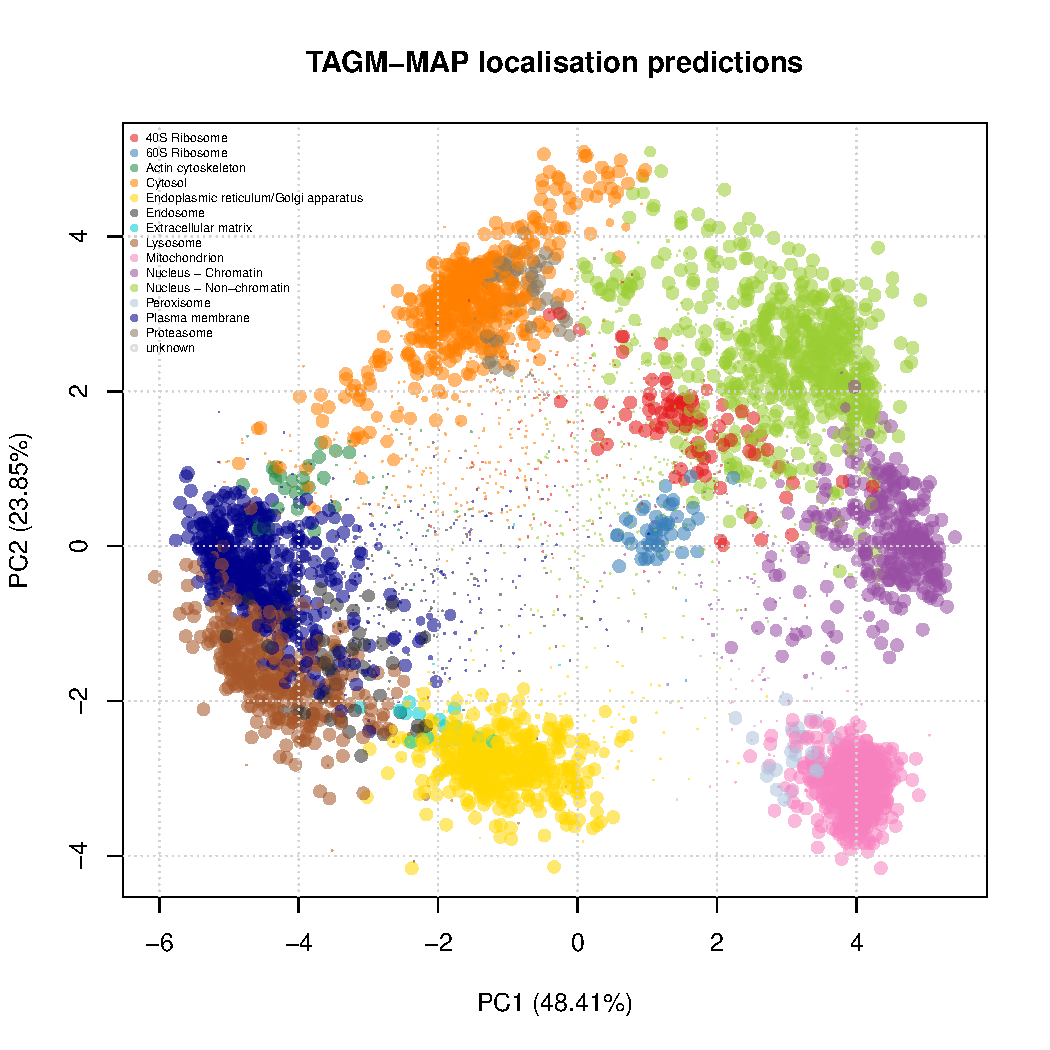
\includegraphics[width=\maxwidth]{figure/assignmentPCAMAP-1} 

\end{knitrout}
    \end{subfigure}%
    \begin{subfigure}[t]{0.5\textwidth}
\begin{knitrout}
\definecolor{shadecolor}{rgb}{0.969, 0.969, 0.969}\color{fgcolor}
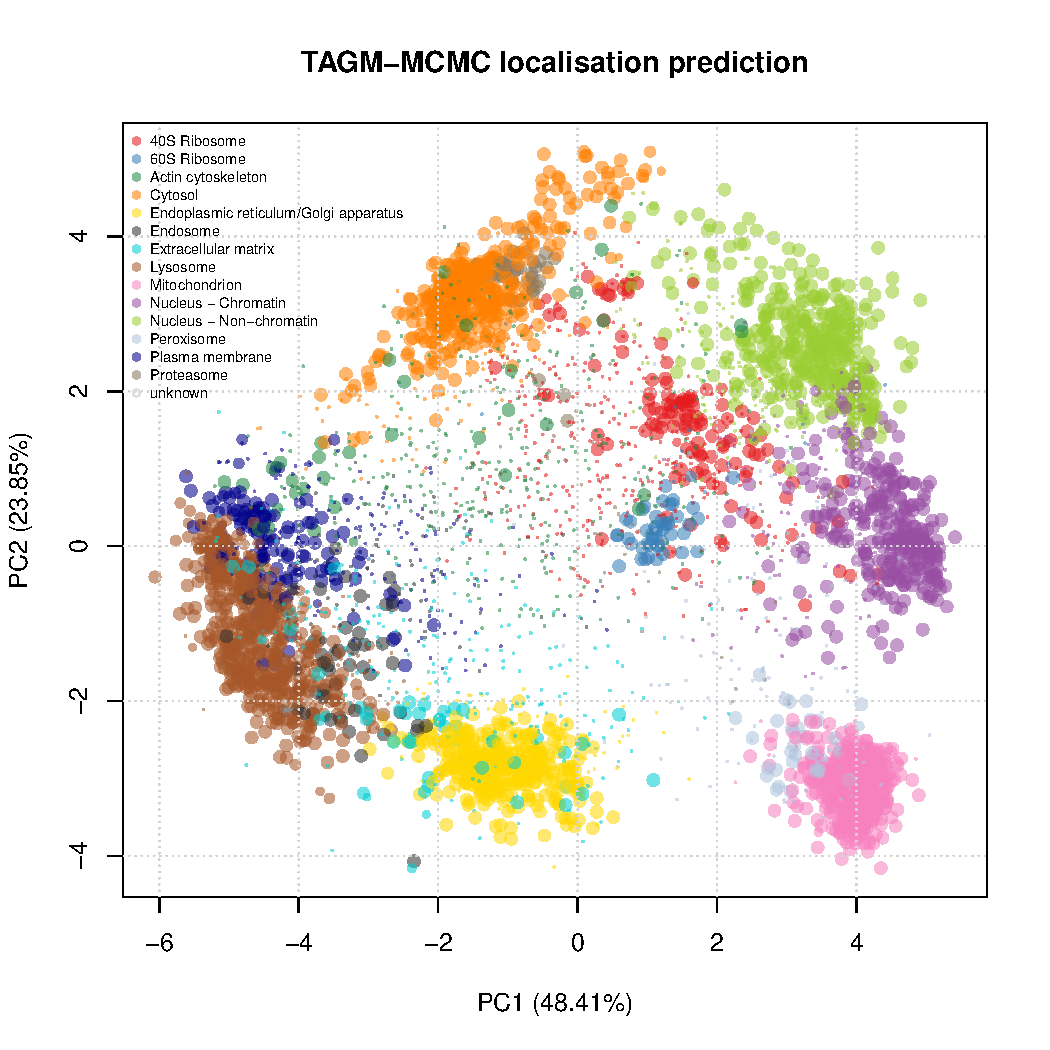
\includegraphics[width=\maxwidth]{figure/assignmentPCAMCMC-1} 

\end{knitrout}
    \end{subfigure}%
  \centering
  \caption{PCA plot of the protein quantitation data with colours
    representing the predicted class (5032 proteins) illustrating
    protein localisation preductions using TAGM-MAP (left) and
    TAGM-MCMC (right) respectively. The pointer size of a protein is
    scaled to the probability that particular protein was assigned to
    that organelle. Markers, proteins whose localisations are already
    known, are automatically assigned a probability of $1$ and the
    size of the pointer reflects this.}
  \label{fig:assignmentPCA} %% MAP and MCMC
\end{figure}


\subsubsection{Uncertainty in the posterior localisation probabilities}

This section applies the TAGM model to the mouse pluripotent embryonic
stem cell data, by considering the uncertainty in the parameters and
exploring how this uncertainty propogates to the uncertainty in
protein localisation prediction.  In figure
\ref{figure::pcaellipseMCMC} we visualise the model as before using
the first two principal components along with the first and fourth
principal component as a representive example.  For the TAGM model, we
derive probability ellipses from the expected value of the posterior
NIW distribution.

We apply the statistical methodology detailed in section
\ref{section:methods}.  We perform posterior computation in the
Bayesian setting using standard MCMC methods (TAGM-MCMC).  We run $6$
chains of our Gibbs sampler in parallel for $15,000$ iterations,
throwing away the first $4,000$ iterations for burn-in and retain
every $10^{th}$ sample for thinning.  Thus 1,100 sample are retained
from each chain. We then visualise the trace plots of our chains; in
particular, we monitor the number of proteins allocated to the known
components (see appendix \ref{app:mcmc}). We discard $1$ chain because
we do not considered it to have converged.  For the remaining $5$
chains we further discard the first $500$ samples by visual
inspection.  We then have $600$ retained samples from $5$ separate
chains. For further analysis, we compute the Gelman-Rubin convergence
diagnostic \citep{Gelman:1992, Brooks:1998}, which is computed as
$\hat{R} \approx 1.05$.  Values of $\hat{R}$ far from 1 indicate
non-convergence and since our statistic is less than $1.1$, we
conclude our chains have converged. The remaining samples are then
pooled to produce a single chain containing $3000$ samples.

We produce point estimates of the posterior localisation probabilities
by summarising samples by their Monte-Carlo average.  These summmaries
are then visualised in figure \ref{fig:assignmentPCA} (right panel),
where the pointer is scaled according to the localisation
probabilities. Monte-Carlo based inference also provides us with
additional information; in particular, we can interrogate individual
proteins and their posterior probability distribution over
sub-cellular locations.

Figure \ref{fig:G5E870} illustrates one example of the importance of
capturing uncertainty.  The E3 ubiquitin-protein ligase TRIP 12
(G5E870) is an integral part of ubiquitin fusion degradation pathway
and is a protein of great interest in cancer because it regulates DNA
repair pathways. The SVM failed to assign this protein to any
location, with assigment to the 60S Ribosome falling below a $5\%$ FDR
and the MAP estimate assigned the protein to the nucleus non-chromatin
with posterior probability < 0.95.  The posterior distribution of
localisation probabilities inferred from the TAGM-MCMC model, shown in
figure \ref{fig:G5E870}, demonstrates that this protein is most
probably localised to the nucleus non-chromatin. However, there is
some uncertainty about whether it localises to the $40$S ribosome.
This could suggest a dynamic role for this protein, which could be
further explored with a more targeted experiment.

\begin{figure}[ht]
  \begin{subfigure}[t]{0.45\textwidth}
        \centering
\begin{knitrout}
\definecolor{shadecolor}{rgb}{0.969, 0.969, 0.969}\color{fgcolor}\begin{kframe}


{\ttfamily\noindent\bfseries\color{errorcolor}{\#\# Error in get(name, envir = asNamespace(pkg), inherits = FALSE): object 'plotEllipse\_old' not found}}

{\ttfamily\noindent\bfseries\color{errorcolor}{\#\# Error in strwidth(legend, units = "{}user"{}, cex = cex, font = text.font): plot.new has not been called yet}}\end{kframe}
\end{knitrout}
        \caption{}
\end{subfigure}%
\hfill
\begin{subfigure}[t]{0.45\textwidth}
\begin{knitrout}
\definecolor{shadecolor}{rgb}{0.969, 0.969, 0.969}\color{fgcolor}\begin{kframe}


{\ttfamily\noindent\bfseries\color{errorcolor}{\#\# Error in get(name, envir = asNamespace(pkg), inherits = FALSE): object 'plotEllipse\_old' not found}}

{\ttfamily\noindent\bfseries\color{errorcolor}{\#\# Error in strwidth(legend, units = "{}user"{}, cex = cex, font = text.font): plot.new has not been called yet}}\end{kframe}
\end{knitrout}
        \centering
        \caption{}
\end{subfigure}
  \centering
  \caption{(a) Probability ellipses produced from using the MCMC
    method.  The density is the expected value from the NIW
    distribution. (b) Probability ellipses visualised along the 1st
    and 4th principal component also from the MCMC method.}
\label{figure::pcaellipseMCMC}
\end{figure}

\begin{figure}[ht]
\centering
\begin{knitrout}
\definecolor{shadecolor}{rgb}{0.969, 0.969, 0.969}\color{fgcolor}

{\centering 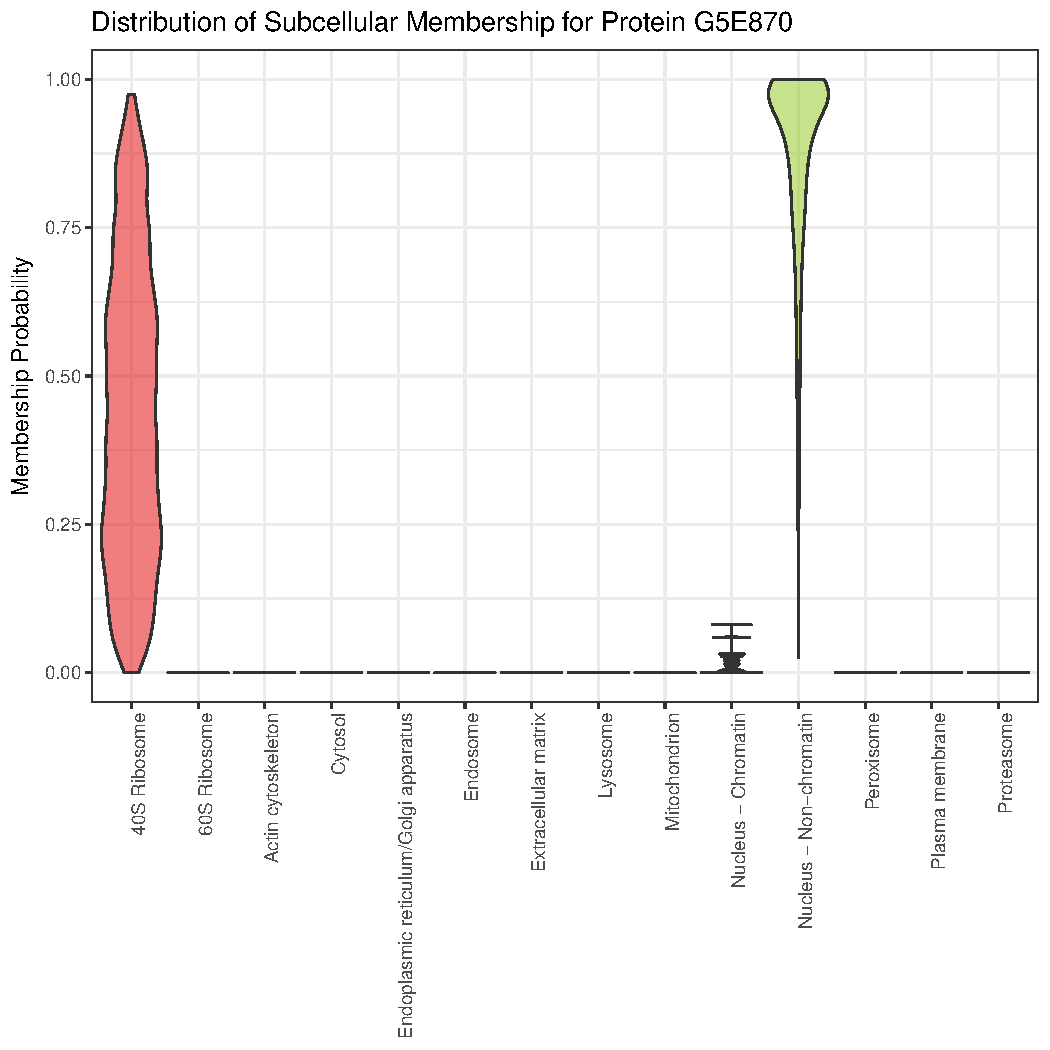
\includegraphics[width=0.7\textwidth]{figure/unnamed-chunk-6-1} 

}



\end{knitrout}

\caption{Violin plot revealing the posterior distribution of
  localisation probabilities of protein E3 ubiquitin-protein ligase
  (G5E870) to organelles and sub-cellular niches.  The most probable
  localisation is nucleus non-chromatin, however there is uncertainty
  associated with this assignment.}
\label{fig:G5E870}
\end{figure}

\clearpage

\subsubsection{Enrichment analysis of outlier proteins}

In previous sections, we have demonstrated that we can assign proteins
probabilitically to sub-cellular compartment and quantify the
uncertainty in these assignments. Some proteins cannot be well
described as belonging to any known component and we modelled this
using an additional t-distribution outlier component.

It is biologically interesting to decipher what functional role
proteins that are far away from known components play. We perform an
over-representation analysis of gene ontology (GO) terms to asses the
biological relevance of the outlier component \citep{Boyle:2004,
  Yu:2012}. We take 1111 proteins that were allocated to known
components with probability less than $0.95$.  Note that these 1111
proteins exclude proteins that are likely to belong to a known
location, but we are uncertain about which localisation.  We then
performed enrichment analysis against the set of all proteins
quantified in the \textit{hyper}LOPIT experiment. We search against
the cellular compartment, biological process and molecular function
ontologies.

Supplementary figure \ref{fig:GOenrich} shows this outlier component
is enriched for cytoskeletal part ($p <10^{-7}$) and microtuble
cytoskeleton ($p <10^{-7}$). Cytoskeleton proteins are found
throughout the cell and therefore we would expect them to be found in
every fraction along the density gradient. We also observe enrichment
for highly dynamic sub-cellular processes such as cell division
($p <10^{-6}$) and cell cycle processes ($p <10^{-6}$), again these
proteins are unlikely to have steady-state locations within a single
component. We also see enrichment for molecular functions such as
tranferase activity $(p < 0.005)$, another highly dynamic
process. These observations justify including an additional outlier
component in our mixture model.


\clearpage

\subsection{Comparison with other classifiers}

In this section, we assess the generalisation performance of our
methods on several datasets, by computing performance metrics
associated with each classifier as detailed in section
\ref{section::assessment}. We compare the SVM and KNN classifiers
alongside the MAP and MCMC approaches detailed in the methods
section. We compute the F1 score and quadratic loss over 100 rounds of
stratified 5-fold cross-validation. The hyperparameter for the KNN
algorithm, the number of nearest neighbours, is optimised via an
additional internal 5-fold cross-validation and the hyperparameters
for the SVM, sigma and cost, are also optimised via internal 5-fold
cross validation \cite{svm:2010}.

We test our methods on the following datasets \textit{Drosophila}
\citep{Tan:2009}, chicken \citep{hall:2009}, mouse pluripotent
embryonic stem cells from \cite{hyper} and \cite{Breckels:2016}, the
human bone osteosarcoma epithelial (U2-OS) cell line
\citep{Thul:2017}, the HeLa cell line of \cite{Itzhak:2016}, the $3$
HeLa cell lines from \cite{Hirst:2018} and $10$ primary fibroblast
datasets from \cite{Jean_Beltran:2016}.  These datasets represent a
great variety of spatial proteomics experiments across many different
workflows.

The two \textit{hyper}LOPIT datasets on mouse pluripotent embryonic
stem cells and the U2-OS cell line use TMT 10-plex labelling and
contain the greatest number of proteins.  Earlier LOPIT experiments on
the \textit{Drosophila} and chicken use iTRAQ 4-plex labelling, whilst
another LOPIT mouse pluripotent embryonic stem cell dataset uses iTRAQ
8-plex. The datasets of \cite{Itzhak:2016} and \cite{Hirst:2018}
employ a different methodology completely - seperating cellular
content using differential centrifugation (as opposed to along a
density-gradient).  Furthermore, the methods use SILAC rather than
iTRAQ or TMT for labelling. The experiments of \cite{Hirst:2018} were
designed to explore the functional role of AP-5 by coupling
CRISPR-CAS9 knockouts with spatial proteomics methods. We analysed all
three datasets from \cite{Hirst:2018}, which includes a wild type HeLa
cell line as a control, as well as two CRISPR-CAS9 knockouts:
AP5Z1-KO1 and AP5Z1-KO2 respectively.

In addition, we analysed the spatio-temporal proteomics experiments of
\cite{Jean_Beltran:2016}, which uses TMT-based MS quantification. This
experiment explored infecting primary fibroblasts with Human
cytomegalovirus (HMCV) and the goal of these experiments was to
explore the dynamic perturbation of host proteins during infection, as
well as the sub-cellular localisation of viral proteins throught the
HCMV life-cycle. They produced spatial maps at different time points:
$24,48,72,96,120$ hours post infection (hpi), as well as mock maps at
these same time points to serve as a control - this results in $10$
different spatial proteomics maps.

In each case, a dataset specific marker list was used, which is
curated specifically for the each cell line. We removed the
"high-curvature ER" annotations from the HeLa dataset
\citep{Itzhak:2016}, as well as the "ER Tubular", "Nuclear pore
complex" and "Peroxisome" annotations from the HeLa CRISPR-CAS9
knockout experiments \citep{Hirst:2018} as there are too few proteins
to correctly perform cross-validation. Table \ref{table:data}
summarises these datasets, including information about number of
quantified proteins, the workflow used and the number of fractions.

\begin{table}[h]
\centering
\begin{tabular}{ |p{3cm}|p{3cm}|p{2cm}|p{2cm}|p{2cm}|  }
 \hline

 \multicolumn{5}{|c|}{MS-based Spatial Proteomics datasets} \\
 \hline
 Cell line or organism & Workflow & Labelling & Fractions (including combined replicates) & Proteins \\
 \hline
 \hline
 \textit{Drosophila}   &  LOPIT & iTRAQ & 4  & 888\\
 \hline
 Chicken DT40 & LOPIT  & iTRAQ & 16 & 1090 \\
 \hline
 Mouse pluripotent E14TG2a stem cell  &  HyperLOPIT & TMT & 20 & 5032\\
 \hline
 HeLa (Itzhak et al.) & Organeller Maps & SILAC & 30 & 3766\\
 \hline
 HeLa (Hirst et al.) & Organeller Maps  & SILAC & 15 & 2046\\
 \hline
 U2-OS cell line & HyperLOPIT  & TMT & 37 & 5020\\
 \hline
 Primary Fibroblast & Spatio-Temporal Methods & TMT & 6 & 2196 \\
 \hline
 E14TG2a (Breckels et al.)  &  LOPIT & iTRAQ & 8 & 2031\\
\hline
\end{tabular}
\caption{Summary of spatial proteomics datasets used for comparisons}
\label{table:data}
\end{table}

Figures \ref{figure::f1scores1} and \ref{figure::f1scores2} compare
the Macro-F1 scores across the datasets for all classifiers and
demonstrates that no single classifier consistently outperforms any
other across all datasets, with results being highly consitent across
all methods, as well as across datasets. We perform a pairwise
unpaired t-test with multiple testing correction applied using the
Benjamini-H\"ochberg procedure \citep{FDR:1995} to detect differences
between classifier performance.

In the \textit{Drosophila} dataset only the KNN algorithm outpeforms
the SVM at significance level of $0.01$, whilst no other significance
difference exist between the classifiers. In the chicken DT40 dataset
only the MCMC method outperforms the KNN classifier at significance
level of $0.01$, no other significant conclusion can be drawn. In the
mouse dataset the MAP based method outperforms the MCMC method at
significant level of $0.01$, no other significant conclusions can be
drawn. In the HeLa dataset all classifiers are significantly different
at a $0.01$ level. These difference may exist because the dataset does
not fit well with our modelling assumptions; in particular, this
dataset set has been curated to have a class called "Large Protein
Complex", which likely describes several sub-cellular
structures. These might include nuclear compartments and ribosomes, as
well as any cytosolic complex and large protein complex which pellets
during the centrifugation conditions used to capture this mixed
sub-cellular fraction. Moreover, the cytosolic and nuclear fraction
were processed separatly leading to possible imbalance with
comparisions with other datasets. Thus, the large protein complex
component might be better described as itself a mixture model or more
detailed curation of these data may be required. We do not consider
further modelling of this dataset in this manuscript. For the U2-OS
all classifiers are significantly different at a significant level of
$0.01$ except for the SVM classifier and the MCMC method, with the MAP
method performing the best. Figure \ref{figure::f1scores1} shows that
for this dataset all classifiers are performing extremely well. In the
three Hirst datasets the MAP method significantly outperforms all
other methods $(p < 0.01)$, whilst in the wild type HeLa and in the
CRISPR-CAS9 KO1 there is no significant difference between the KNN
and MCMC method. In the CRISPR-CAS9 KO2 the MCMC method outperforms
the SVM and KNN methods (p < 0.01). In the interest of brevity, the
remaining results for the t-tests can be found in tables in appendix
\ref{app::ttestf1}.




\begin{figure}[ht]
  \centering
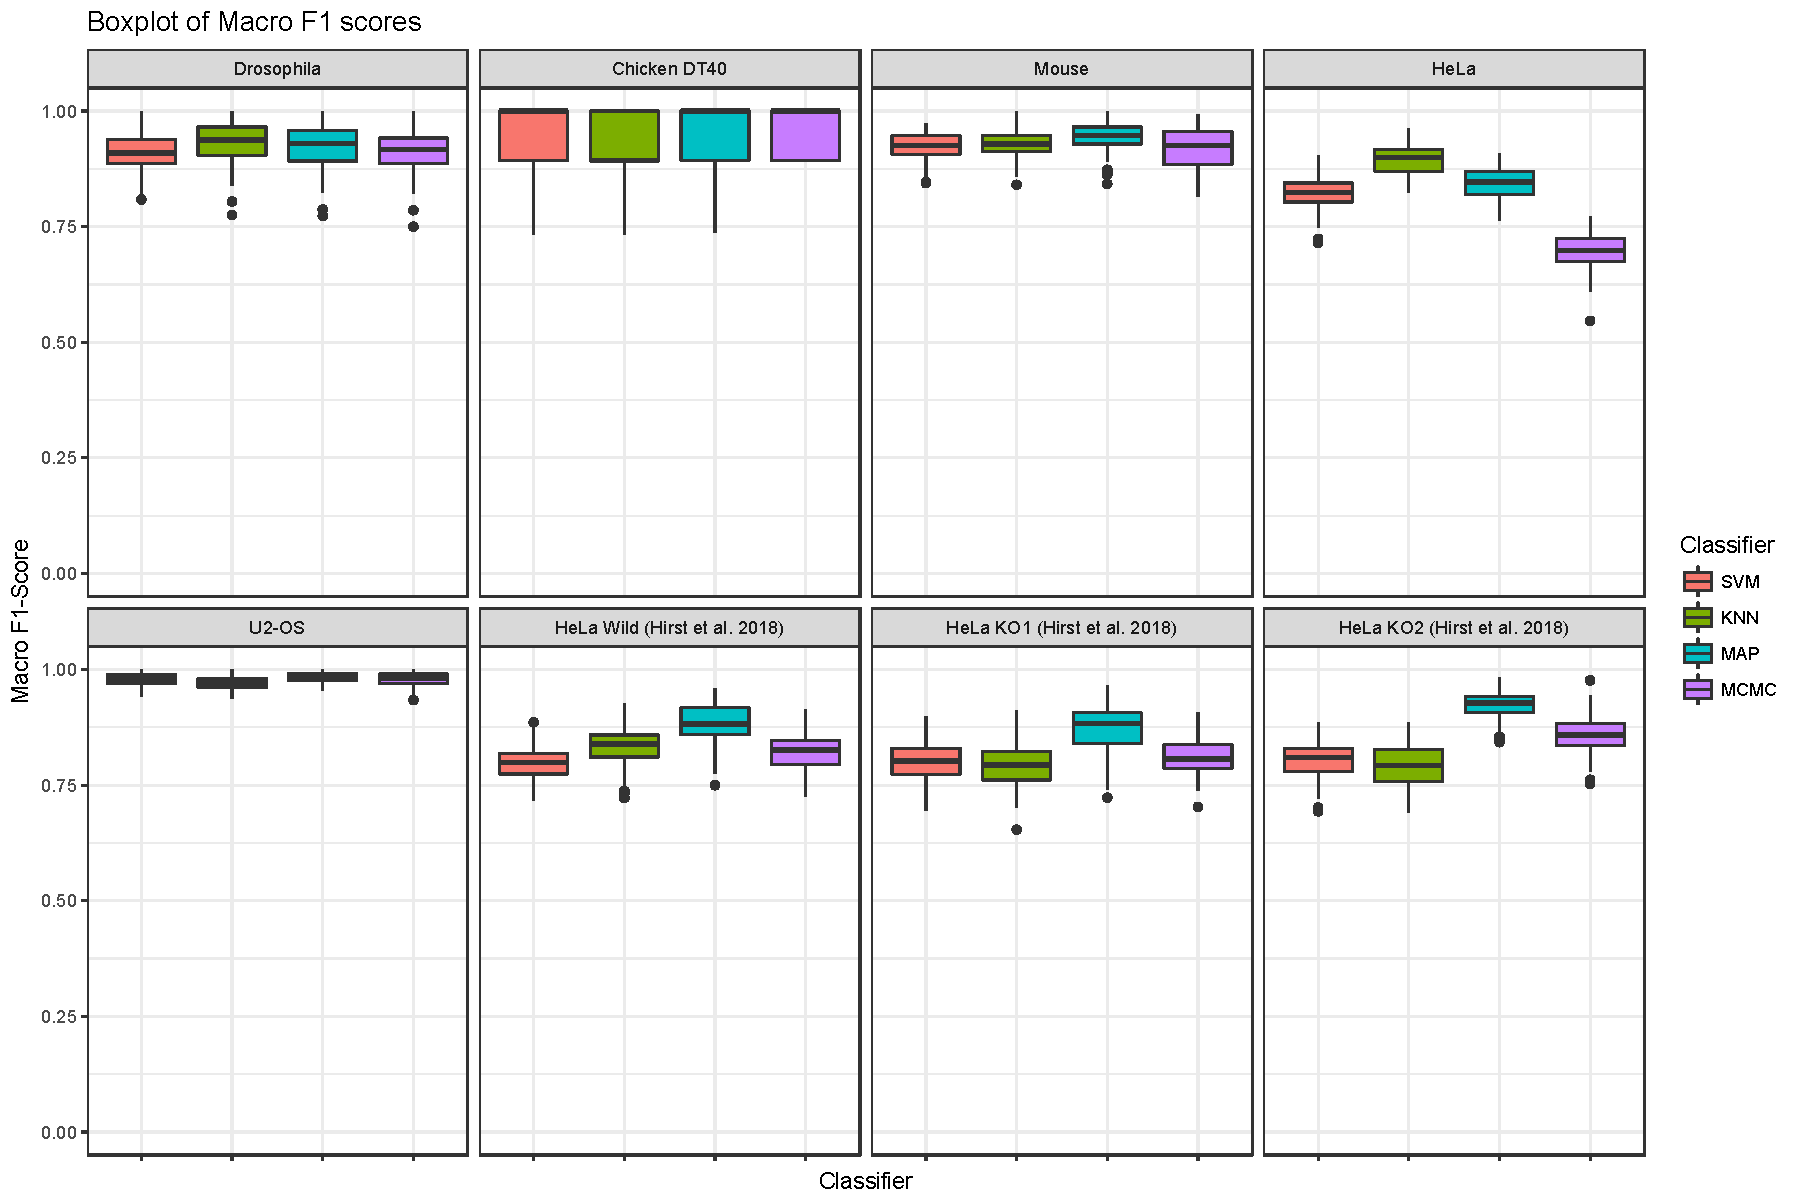
\includegraphics[width=0.8\textwidth]{F1compare1.pdf}
  \caption{Boxplots of the distributions of Macro F1 scores
    for 8 different spatial proteomics datasets}
  \label{figure::f1scores1}
\end{figure}

\begin{figure}[ht]
  \centering
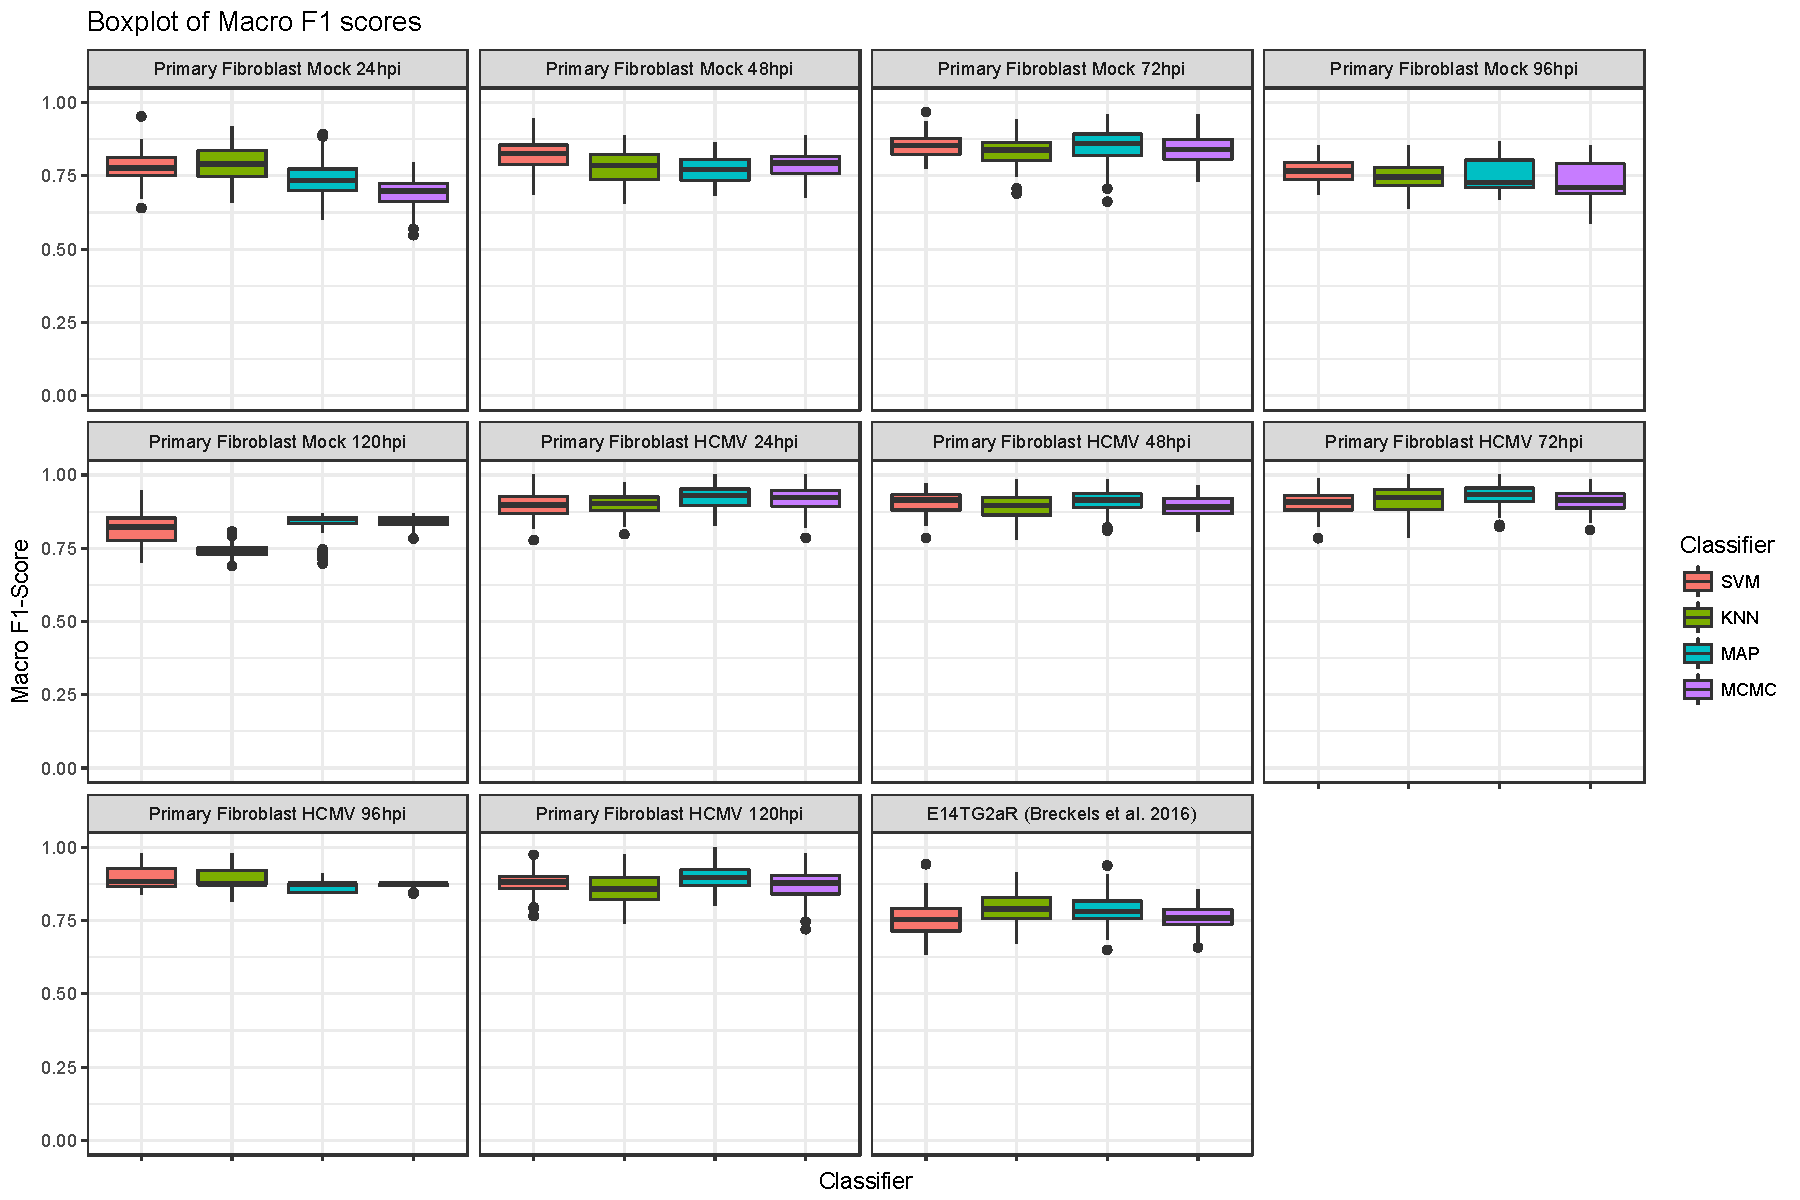
\includegraphics[width=0.8\textwidth]{F1comparisons2.pdf}
  \caption{Boxplots of the distributions of Macro F1 scores
    for 10 spatial-temporal proteomics datasets on primary fibroblast cell,
    as well as a LOPIT spatial proteomics dataset on the E14TG2a cell line }
  \label{figure::f1scores2}
\end{figure}

\clearpage

The Macro-F1 scores do not take into account that whilst the
TAGM model may misclassify, it may do so with low confidence. We
therefore additionally compute the quadratic loss, which allows
us to make use of the probabilitic information provided
by the classifiers. The lower the quadratic loss the closer the
probabilitic predicition is to the true value. We plot the
distributions of quadratic losses for each classifier in figures
\ref{figure::quadloss1} and \ref{figure::quadloss2}. We observe highly
consitent performance across all classifiers across all
datasets. Again, we perform a pairwise unpaired t-test with multiple
testing correction.

We find that in 16 out of 19 datasets the MCMC methods achieves the
lowest quadratic loss at a signifiance level $<0.0001$ over the SVM
and KNN classifiers. In 6 out of these 16 datasets there is no
significant difference between the MCMC and the MAP methods. In the
three Hirst datasets in which the MCMC did not acheive the lowest
quadratic loss, the SVM outperformed. However, in two of these
datasets (HeLa Wild and KO1) the MAP method and SVM classifier were
not significantly different. In the Hirst KO2 dataset there were no
signicant differences between the MAP and MCMC methods.

In the vast majority of cases, we observe that if the TAGM model,
using the MCMC methdology, makes an incorrect classification it does
so with lower confidence than the SVM classifier, the KNN classifier
and the MAP based classifier, whilst if it is correct in its assertion
it does so with greater confidence. Additionally, a fully Bayesian
methodology provides us with not only point estimates of
classification probabilities but uncertainty quantification in these
allocations, and we show in the following section that this provides
deeper insights into protein localisation.



\begin{figure}[ht]
  \centering
  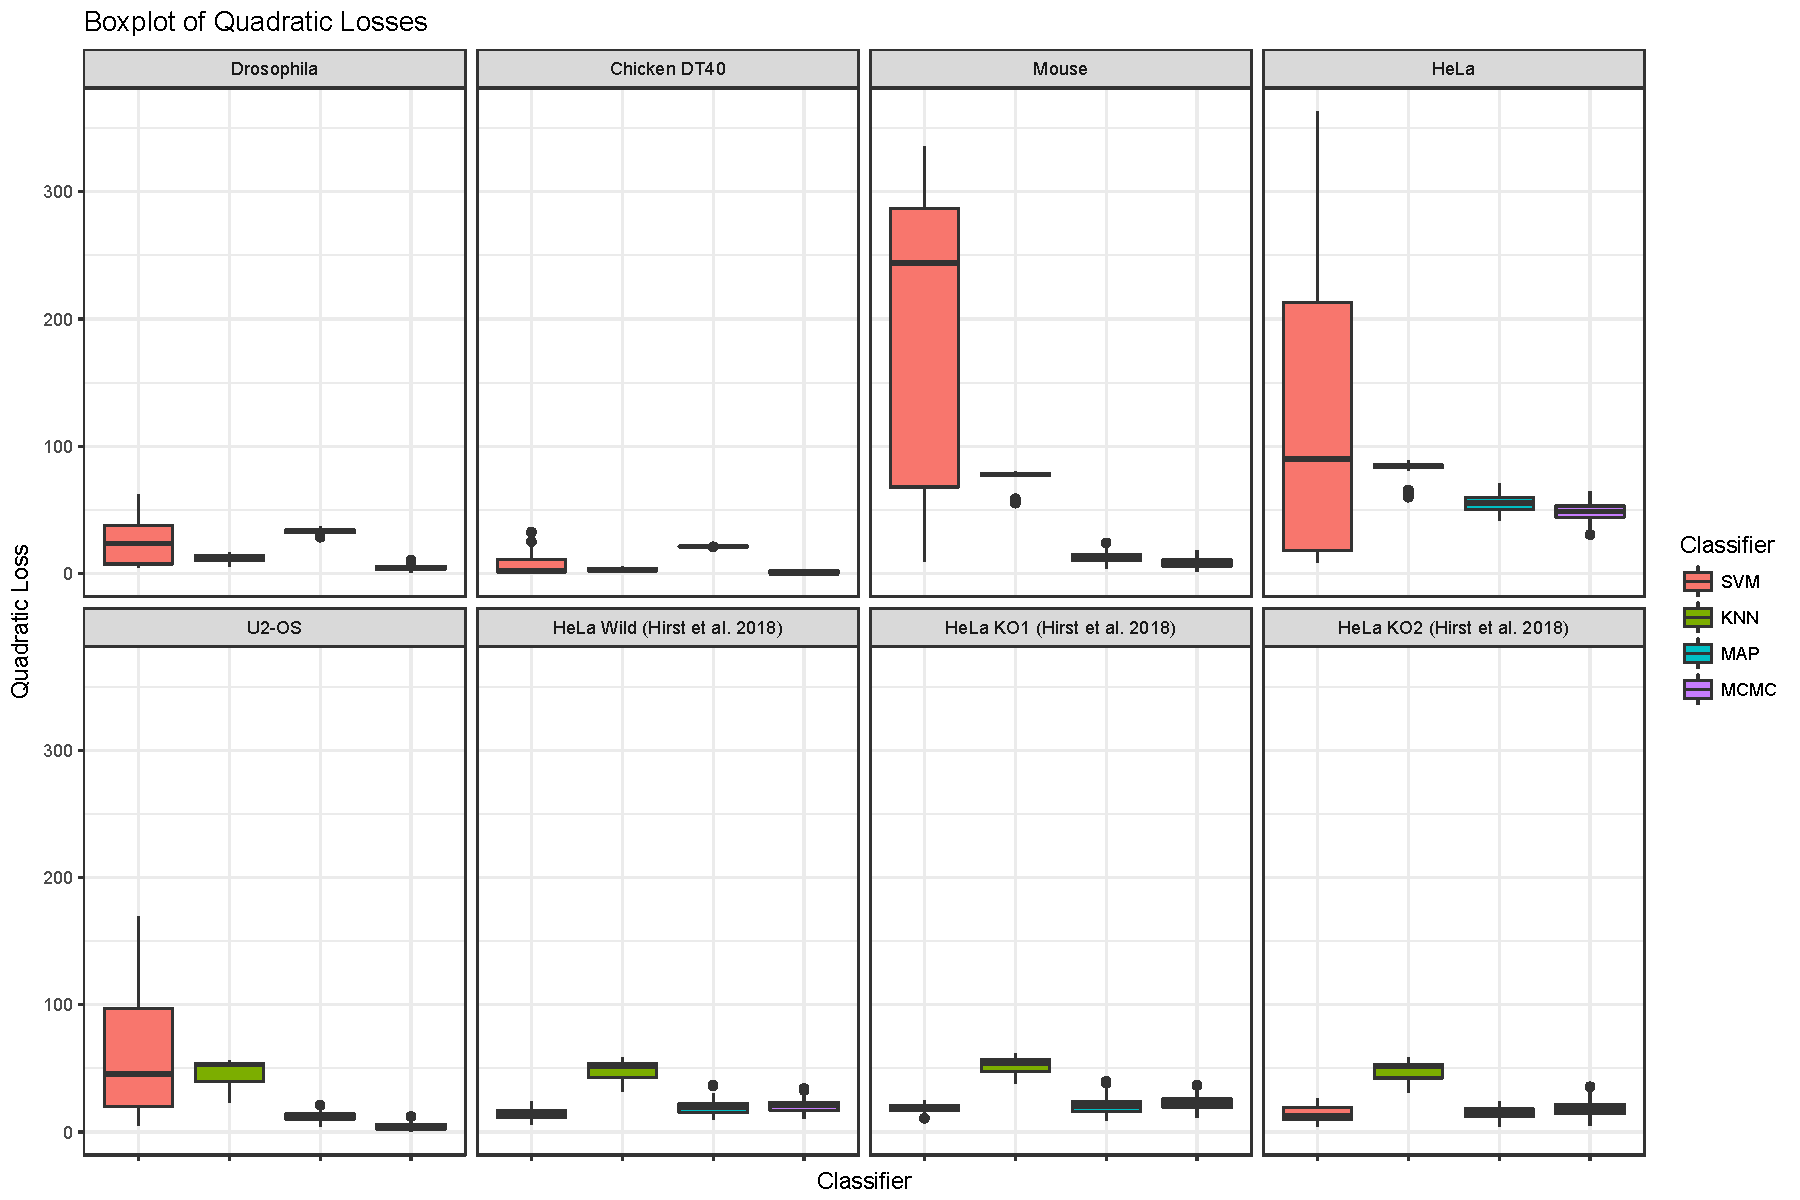
\includegraphics[width=0.8\textwidth]{Quadlosscompare1.pdf}
  \caption{Boxplots of the distributions of Quadratic losses
    for 8 different spatial proteomics datasets}
  \label{figure::quadloss1}
\end{figure}

\begin{figure}[ht]
  \centering
  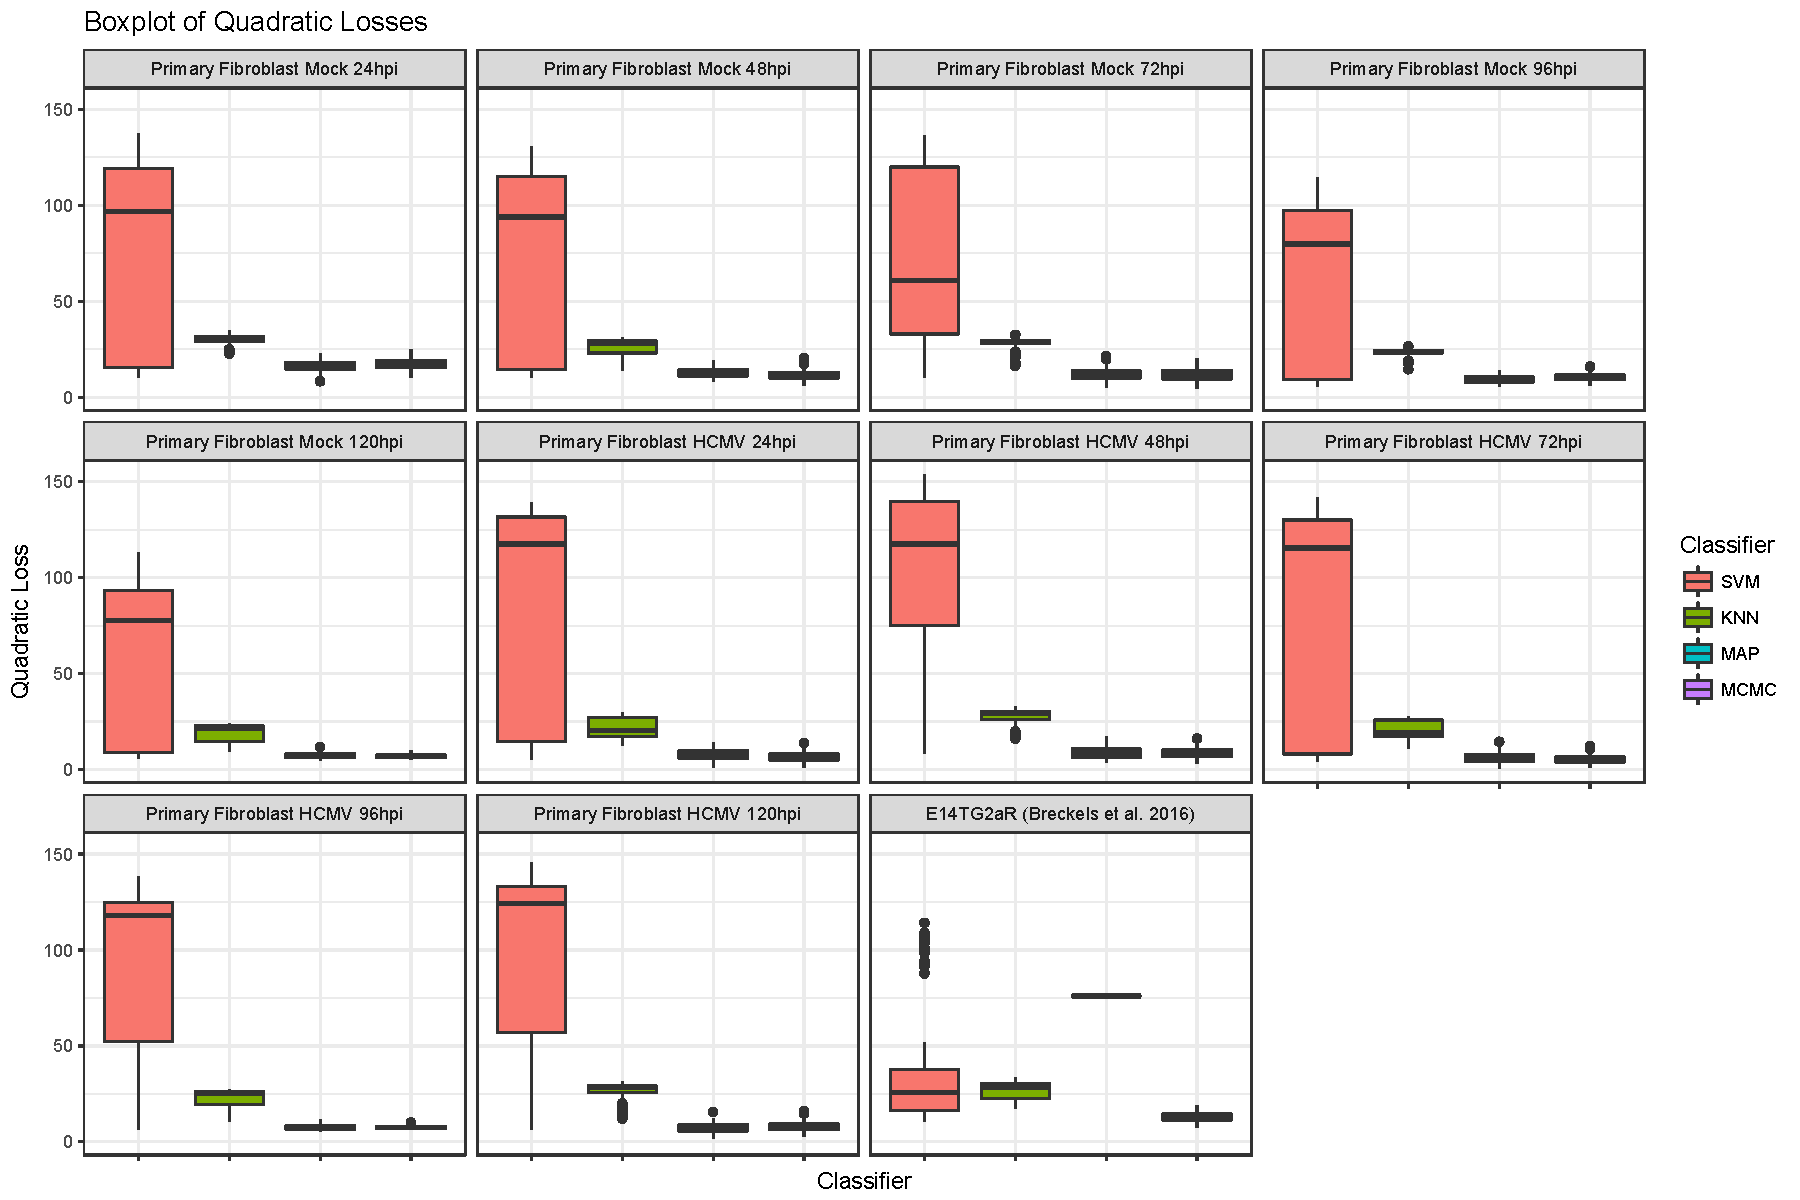
\includegraphics[width=0.8\textwidth]{Quadlosscompare2.pdf}
  \caption{Boxplots of the distributions of Quadratic losses
    for 10 spatial-temporal proteomics datasets on primary fibroblast cell,
    as well as a spatial proteomics dataset on the E14TG2a cell line}
  \label{figure::quadloss2}
\end{figure}


\clearpage

Computing distributions of F1 scores and quadratic losses, which can only be done
on the marker proteins, can help us
understand whether a classifier might have greater generalised
performance accuracy. However, we are interested in whether there is a
large disagreement between classifiers when prediction is performed on
proteins for which we have no withheld localisation information. This
informs us about a systematic bias for a particular classifier or
whether a classifier ensemble could increase performance. To maintain
a common set of proteins we set thresholds for each classifier in turn
and compare to the other classifier without thresholding. Firstly, we
set a global threshold of 0.95 for the TAGM and then for these
proteins plot a contingency table against the classification results
from the SVM. Secondly, we set a 5\% FDR for the SVM and then for
these proteins plot a contingency table against the classification
results from the TAGM. We visualise the contingency tables as heat
plots in figure \ref{figure:contigencytables}.





\begin{figure}[ht]
  \begin{subfigure}[t]{0.5\textwidth}
        \centering
\begin{knitrout}
\definecolor{shadecolor}{rgb}{0.969, 0.969, 0.969}\color{fgcolor}
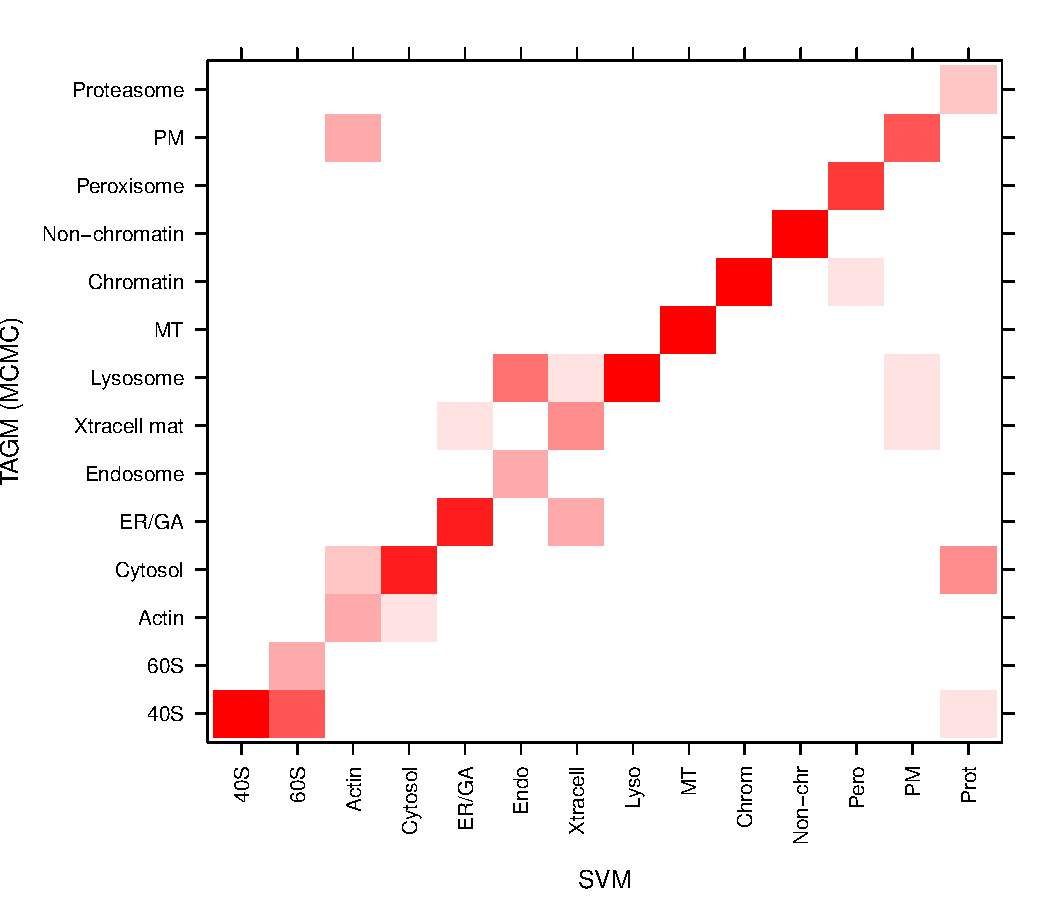
\includegraphics[width=\maxwidth]{figure/unnamed-chunk-10-1} 

\end{knitrout}
\end{subfigure}%
\begin{subfigure}[t]{0.5\textwidth}
\centering
\begin{knitrout}
\definecolor{shadecolor}{rgb}{0.969, 0.969, 0.969}\color{fgcolor}
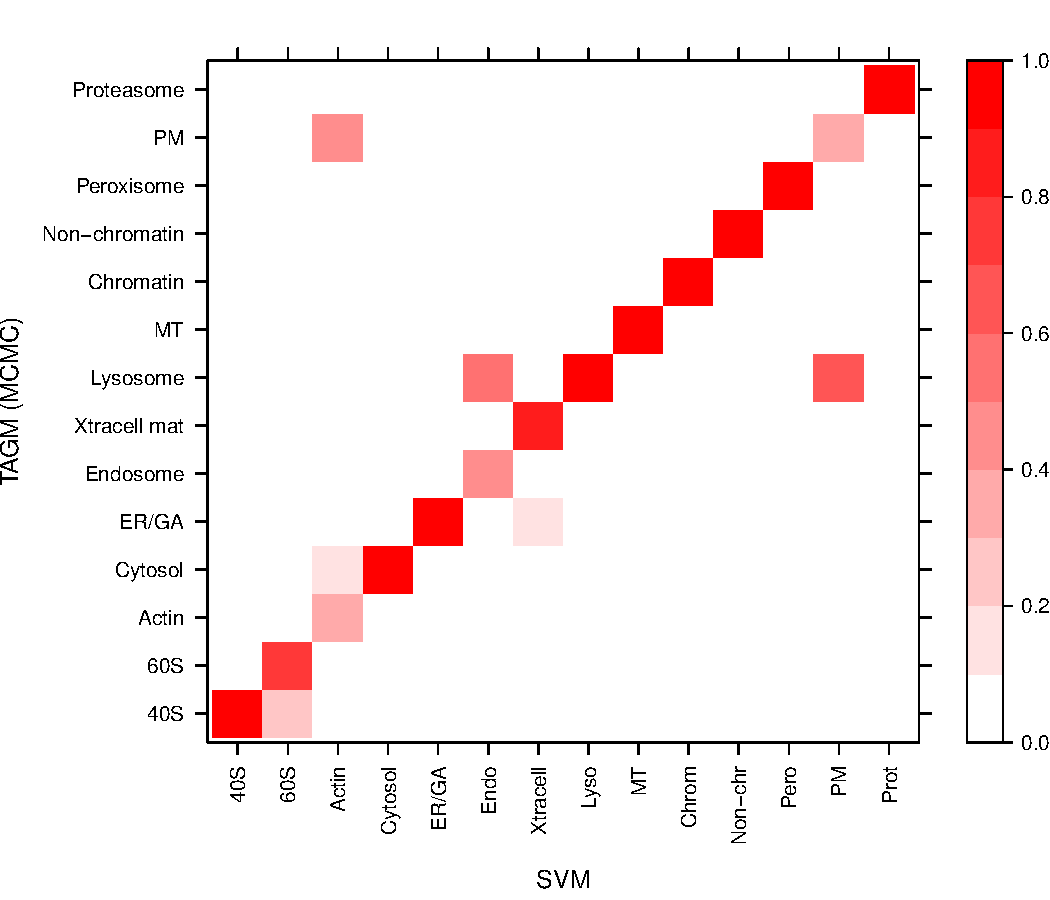
\includegraphics[width=\maxwidth]{figure/unnamed-chunk-11-1} 

\end{knitrout}
\end{subfigure}
  \caption{A heatmap representation of a contingency table,
    where we compare assignment results for proteins
    with unknown protein localisation using the TAGM and
    SVM. The scale ranges from 0 to 1 with values indicating
    the proportion of assigned proteins to that
    sub-cellular location. Values along the diagonal
    represent agreement between classifiers whilst other values
    represent disagreement. The coherence between the classifers is
    very high.
    (a)  In this case we set a probability threshold of 0.95
    for the TAGM assignments with no threshold for the SVM.
    (b)  In this case we set a 5\% FDR threshold for the SVM and
    no threshold for the TAGM.}
\label{figure:contigencytables}
\end{figure}

In general, we see an extremely high level of coherence between the
TAGM and the SVM, with almost all proteins predicted to concordant
sub-cellular compartments. Figure \ref{figure:contigencytables} shows
there is some disagreement between assigning proteins to the lysosome
and plasma membrane, to the cytosol and proteasome,and between the
large and small ribosomal subunits.  However, we have not used the
uncertainty in the probabilitic assignments to produce the contingency
tables above. In the next sections, we explore examples of proteins
with uncertainty in their posterior localisation
probabilities. Selecting biologically relevant thresholds is important
for any classifier and exploring uncertainty is of vital importance
when drawing biological conclusions.


\subsection{Interpreting and exploring uncertainty}

Protein sub-cellular localisation can be uncertain for a number of
reasons. Technical variations and unknown biological novelty, such as
yet uncharacterised functional compartments, can be some of the
reasons why a protein might have an unknown or uncertain
localisation. Furthermore many proteins are known to reside in
multiple locations with possibly different functional duties in each
location. With these considerations in mind, it is pertinant to
quantify the uncertainty in our allocation of proteins to organelles.
This section explores several situations where proteins display
uncertain localisation and considers the biological factors that
influence uncertainty.  We later explore and visualise whole proteome
uncertainty quantification.

\bigskip

Exportin 5 (Q924C1) forms part of the micro-RNA export machinery of
the nucleus, transporting miRNA from the nucleus to the cytoplasm for
further processing.  It then translocates back through the nuclear
pore complex to return to the nucleus.  Exportin 5 can then continue
to mediate further transport between nucleus and cytoplasm.  The SVM
was unable to assign a localisation of Exportin 5, with its assignment
falling below a $5\%$ FDR to wrongly assign this protein to the
proteasome. This incorrect assertion by the SVM was confounded by the
similarity between the cytosol and proteasome profiles.  Figure
\ref{fig:Q924C1} demonstrates, according to the TAGM model, that
Exportin 5 most likely localises to the cytosol but there is some
uncertainty with this assignment.  This uncertainty is reflected in
possible assignment of Exportin 5 to the nucleus non-chromatin and
this uncertainty is a characterisation of the shuttling of this
protein between nucleus and cytoplasm.

The Phenylalanine--tRNA ligase beta subunit protein (Q9WUA2) has an
uncertain localisation between the 40S ribosome and the nucleus
non-chromatin demonstrated in figure \ref{fig:Q9WUA2}. This protein
was left unclassified by the SVM because its score fell below a $5\%$
FDR threshold to assign it to the 40S ribosome. Considering that this
protein is involved in the acylation of transfer RNA (tRNA) with the
amino acid phenylalanine to form tRNAPhe to be used in translation of
proteins, it is therefore unsurprising that this protein's steady
state location is ribosomal.  Whilst the SVM is unable to make an
assignment, TAGM is able to suggest an assignment and quantify our
uncertainty.

Relatively little is known about the Dedicator of cytokinesis (DOCK)
protein 6 (Q8VDR9), a guanine nucleotide exchange factor for CDC42 and
RAC1 small GTPases. The SVM could not assign localisation to the
ER/Golgi, since its score fell below a $5\%$ FDR. Furthermore, the
TAGM model assigned this DOCK 6 to the outlier component with
posterior probability $>0.95$.  Figure \ref{fig:Q8VDR9} shows possible
localisation to several components along the secretory pathway. As an
activator for CDC42 and RAC1 we may expect to see them with similar
localisation. CDC42, a plasma membrane associated protein, regulates
cell cycle and division and is found with many
localisations. Furthermore RAC1, a small GTPase, also regulates many
cellular processes and is found in many locations. Thus the
steady-state distribution of DOCK6 is unlikely to be in a single
location, since its interaction partners are found in many
locations. This justifies including an outlier component in our model,
else we may erroneously assign such proteins to a single location.


\begin{figure}[h]
  \centering
  \begin{subfigure}[t]{0.5\textwidth}
    \centering
\begin{knitrout}
\definecolor{shadecolor}{rgb}{0.969, 0.969, 0.969}\color{fgcolor}

{\centering 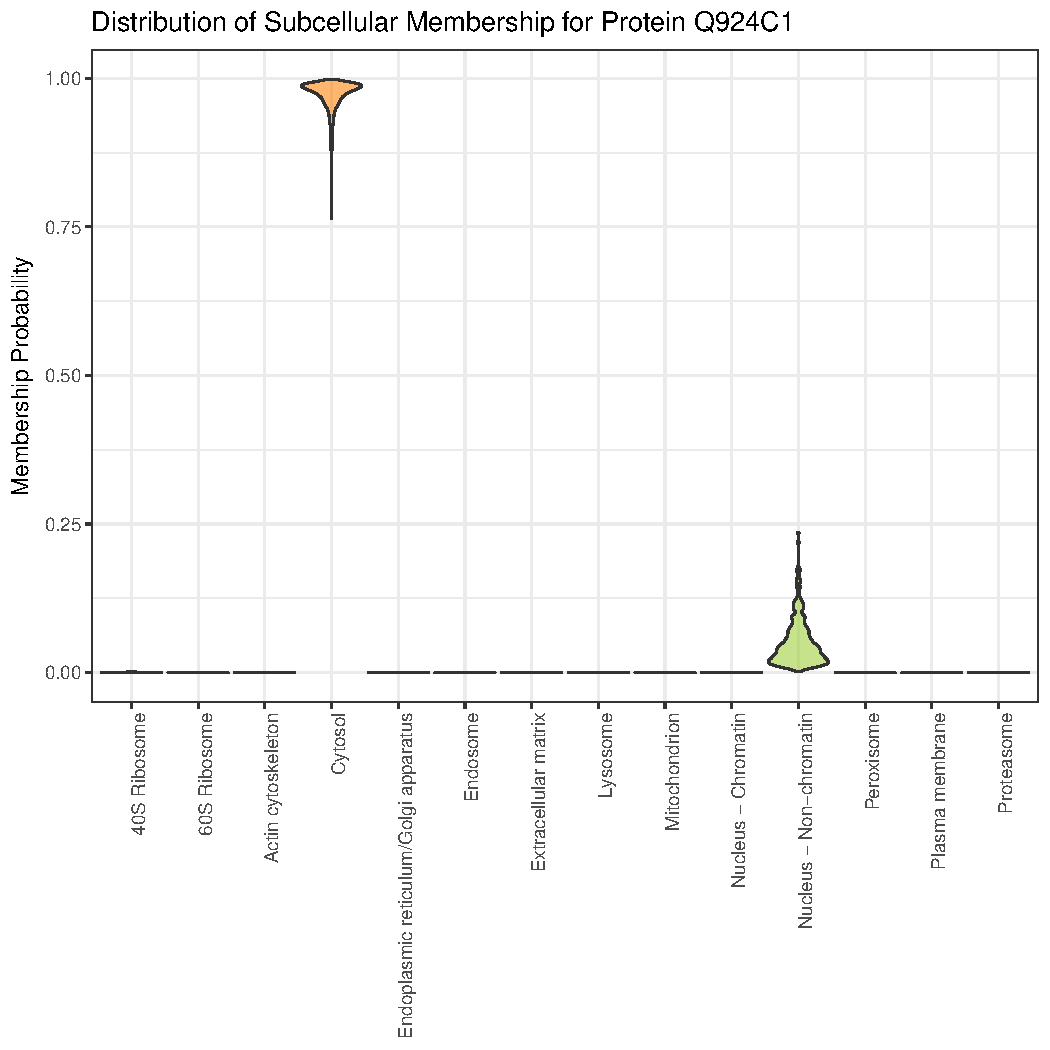
\includegraphics[width=\maxwidth]{figure/unnamed-chunk-12-1} 

}



\end{knitrout}
    \caption{}
  \end{subfigure}%
  \begin{subfigure}[t]{0.5\textwidth}
    \centering
\begin{knitrout}
\definecolor{shadecolor}{rgb}{0.969, 0.969, 0.969}\color{fgcolor}

{\centering 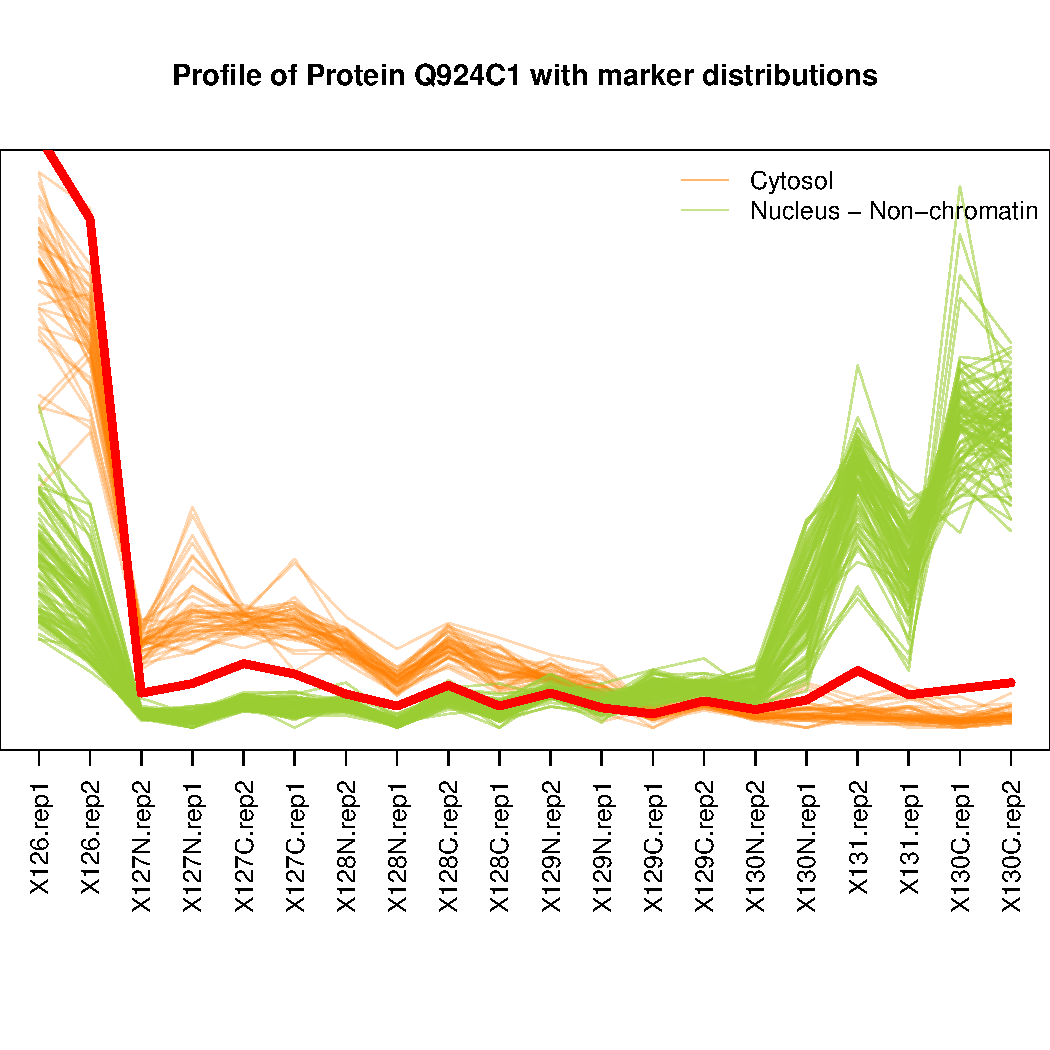
\includegraphics[width=\maxwidth]{figure/unnamed-chunk-13-1} 

}



\end{knitrout}
    \caption{}
  \end{subfigure}
  \vspace{1cm}
  \begin{subfigure}[t]{0.5\textwidth}
    \centering
\begin{knitrout}
\definecolor{shadecolor}{rgb}{0.969, 0.969, 0.969}\color{fgcolor}

{\centering 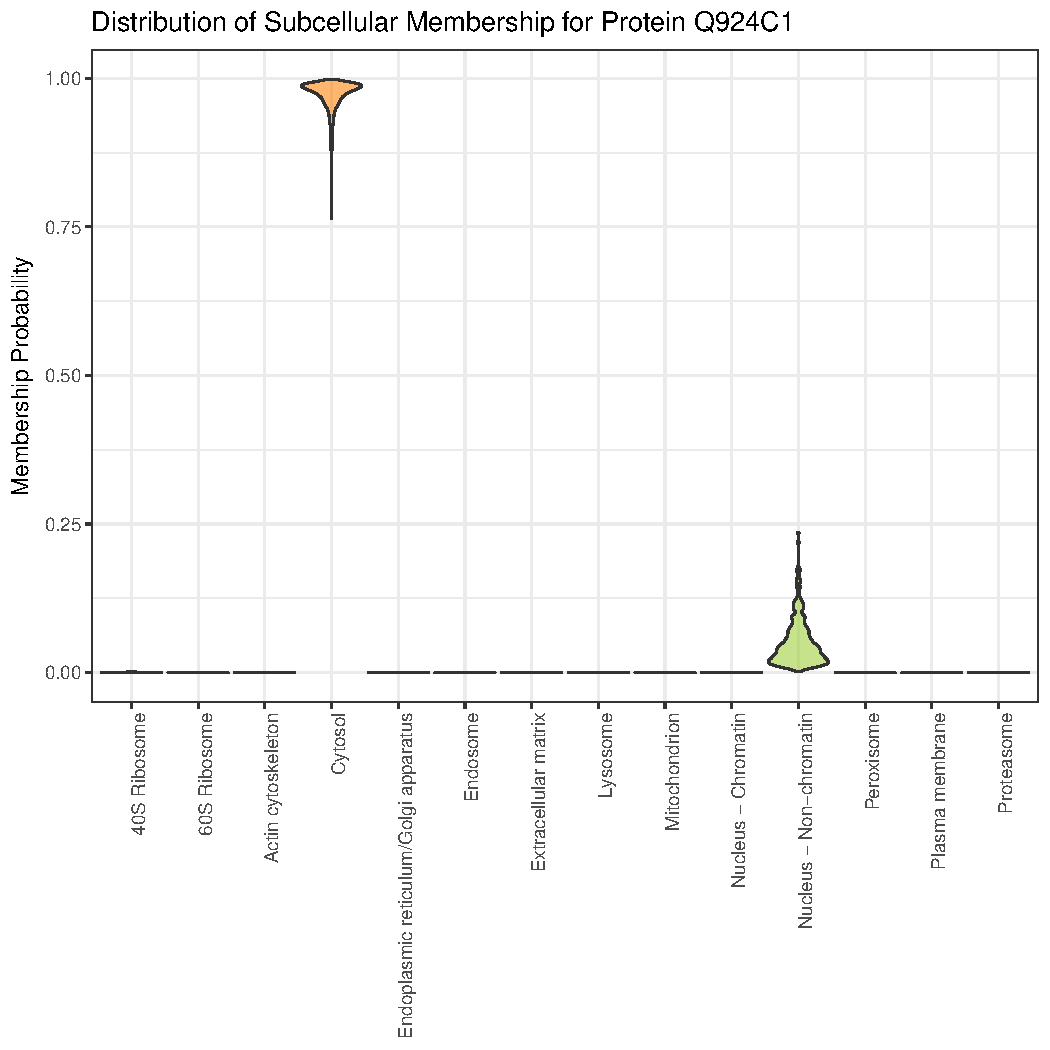
\includegraphics[width=\maxwidth]{figure/unnamed-chunk-14-1} 

}



\end{knitrout}
    \caption{}
  \end{subfigure}%
  \begin{subfigure}[t]{0.5\textwidth}
    \centering
\begin{knitrout}
\definecolor{shadecolor}{rgb}{0.969, 0.969, 0.969}\color{fgcolor}
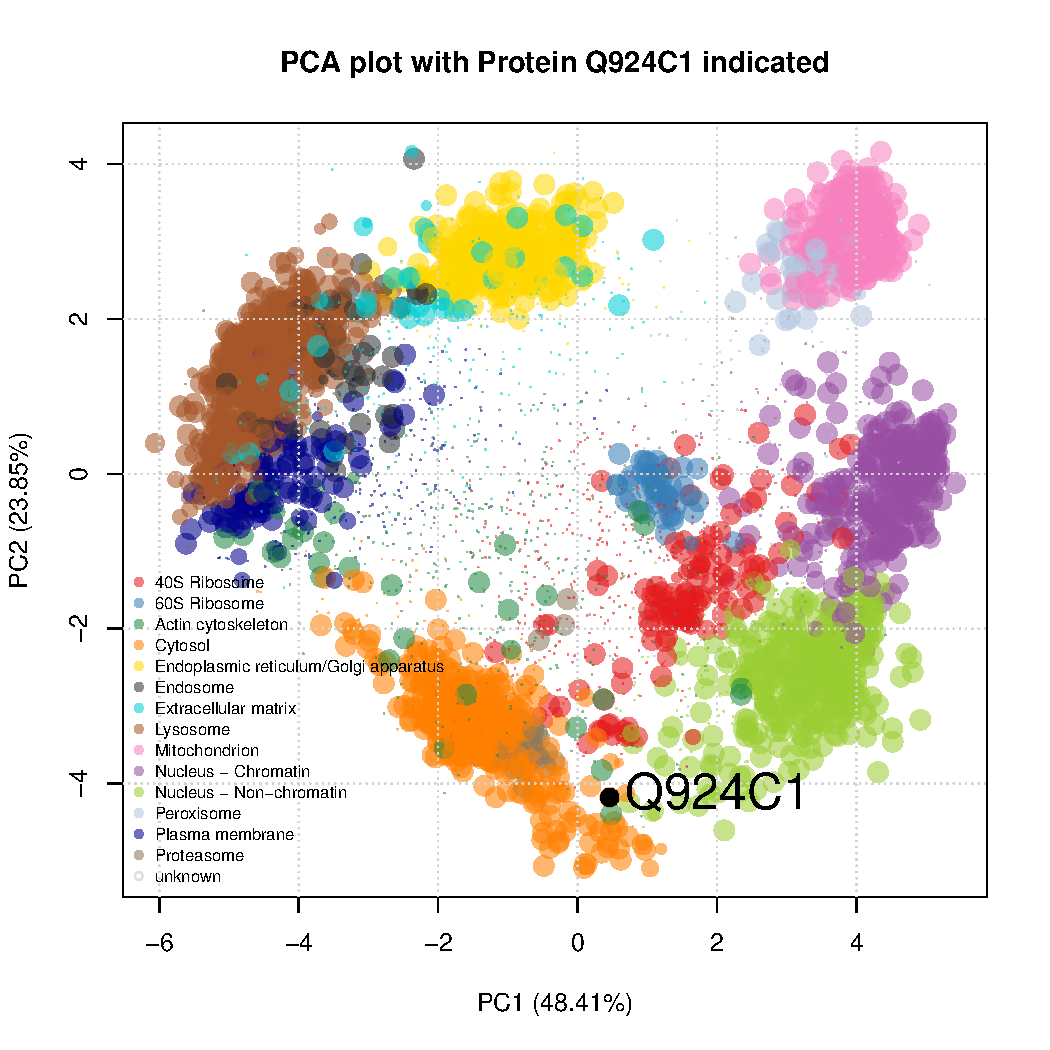
\includegraphics[width=\maxwidth]{figure/unnamed-chunk-15-1} 

\end{knitrout}
    \caption{}
  \end{subfigure}

  \caption{Exportin 5 (Q924C1) showing localisation to the cytosol
    with some uncertainty about association to the nucleus
    non-chromatin.  (a) The violin plot shows uncertain localisation
    between these two sub-cellular localisations. (b) The quantitative
    profile of this protein shows mixed profile between the profiles
    of the organelle markers. (c) The density plot shows a complex
    distribution over localisations for this protein. (d) The protein
    Q924C1 has steady state distribution between the cytosol and
    nucleus non-chromatin.}
  \label{fig:Q924C1}
\end{figure}

\begin{figure}[h]
  \centering
  \begin{subfigure}[t]{0.5\textwidth}
    \centering
\begin{knitrout}
\definecolor{shadecolor}{rgb}{0.969, 0.969, 0.969}\color{fgcolor}

{\centering 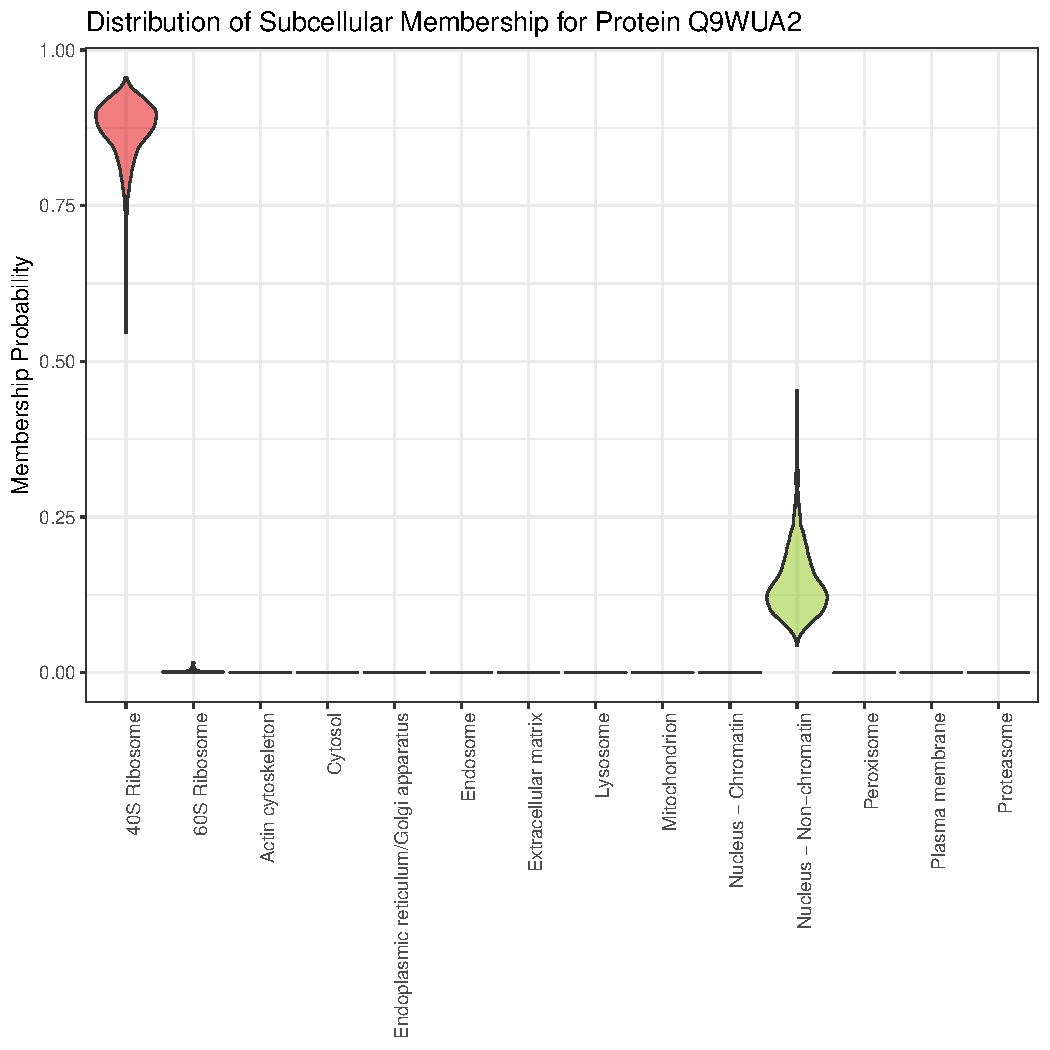
\includegraphics[width=\maxwidth]{figure/unnamed-chunk-16-1} 

}



\end{knitrout}
    \caption{}
  \end{subfigure}%
  \begin{subfigure}[t]{0.5\textwidth}
    \centering
\begin{knitrout}
\definecolor{shadecolor}{rgb}{0.969, 0.969, 0.969}\color{fgcolor}

{\centering 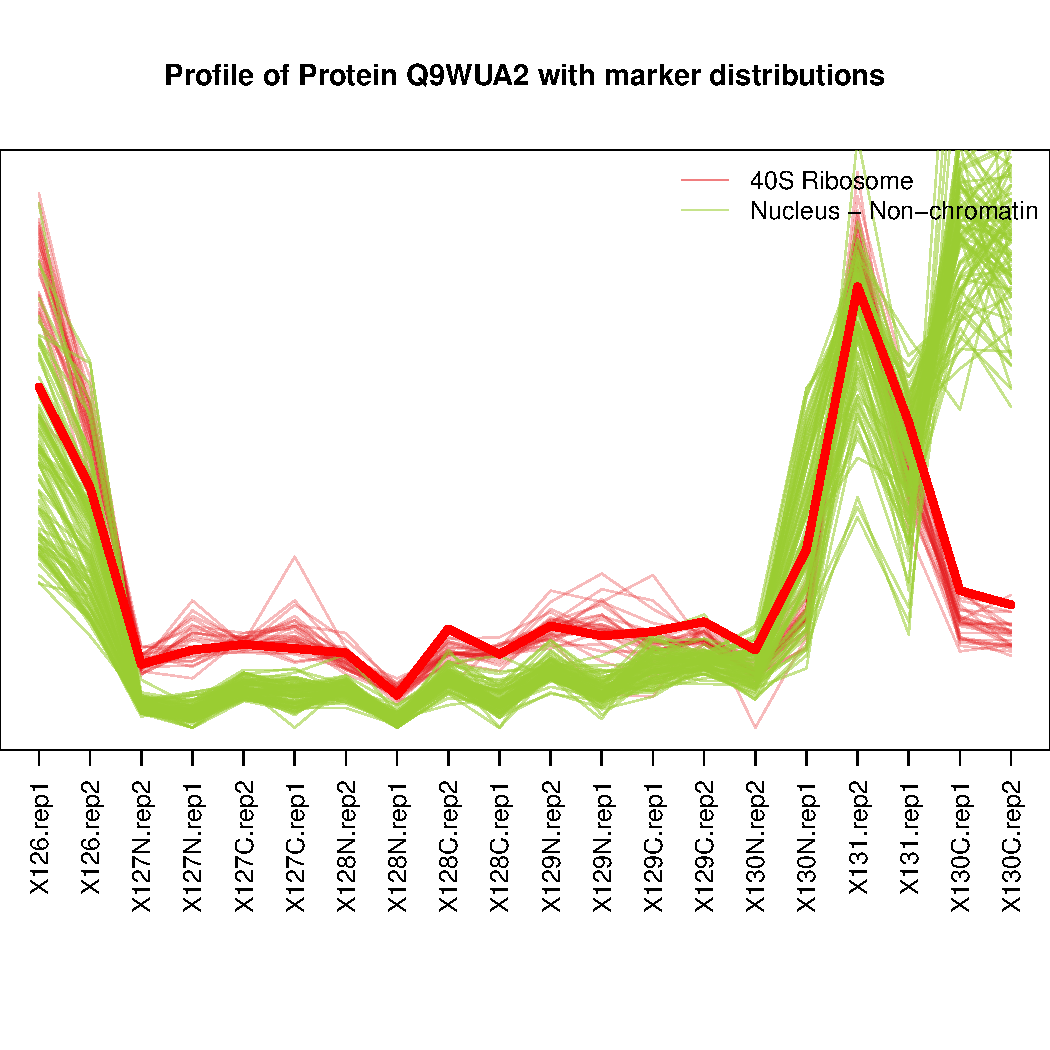
\includegraphics[width=\maxwidth]{figure/unnamed-chunk-17-1} 

}



\end{knitrout}
    \caption{}
  \end{subfigure}
  \vspace{1cm}
  \begin{subfigure}[t]{0.5\textwidth}
    \centering
\begin{knitrout}
\definecolor{shadecolor}{rgb}{0.969, 0.969, 0.969}\color{fgcolor}

{\centering 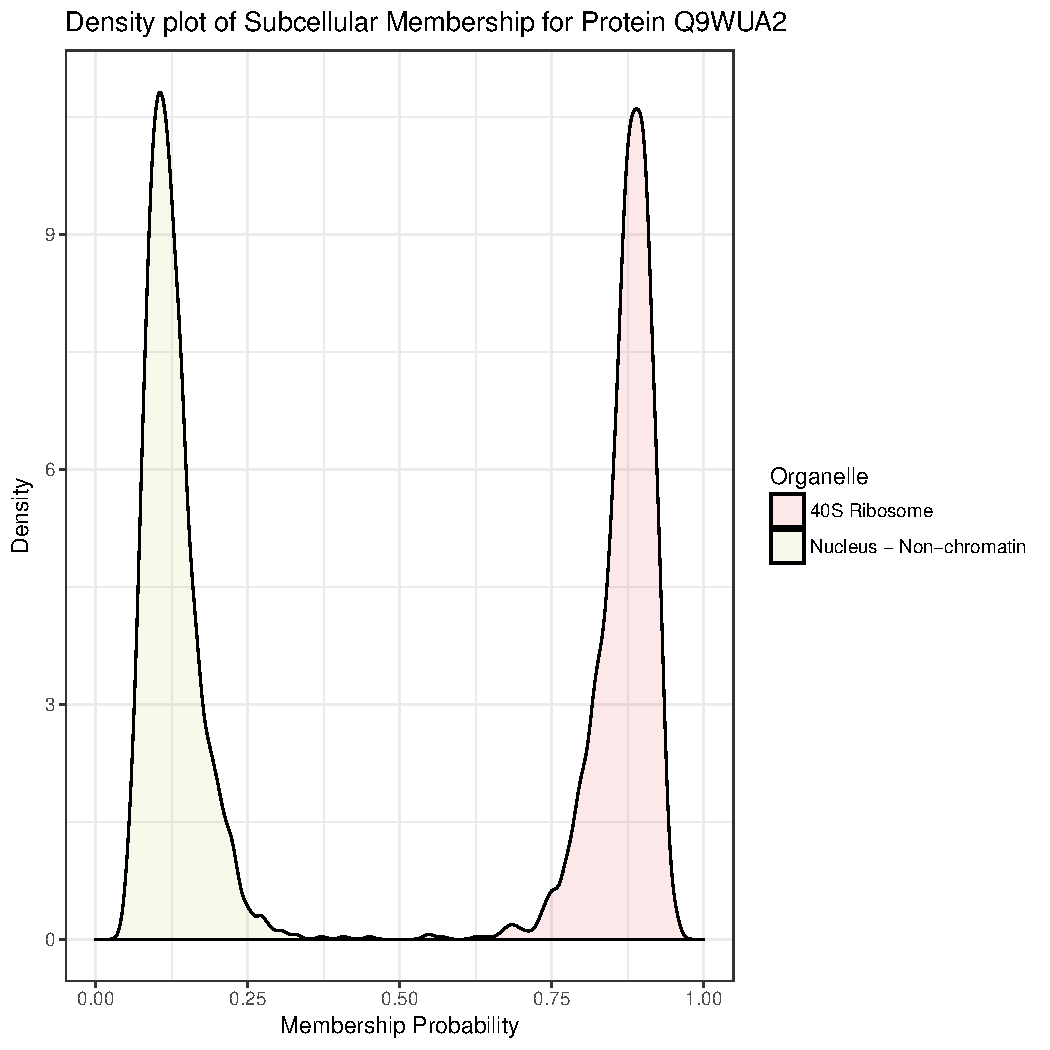
\includegraphics[width=\maxwidth]{figure/unnamed-chunk-18-1} 

}



\end{knitrout}
    \caption{}
  \end{subfigure}%
  \begin{subfigure}[t]{0.5\textwidth}
    \centering
\begin{knitrout}
\definecolor{shadecolor}{rgb}{0.969, 0.969, 0.969}\color{fgcolor}

{\centering 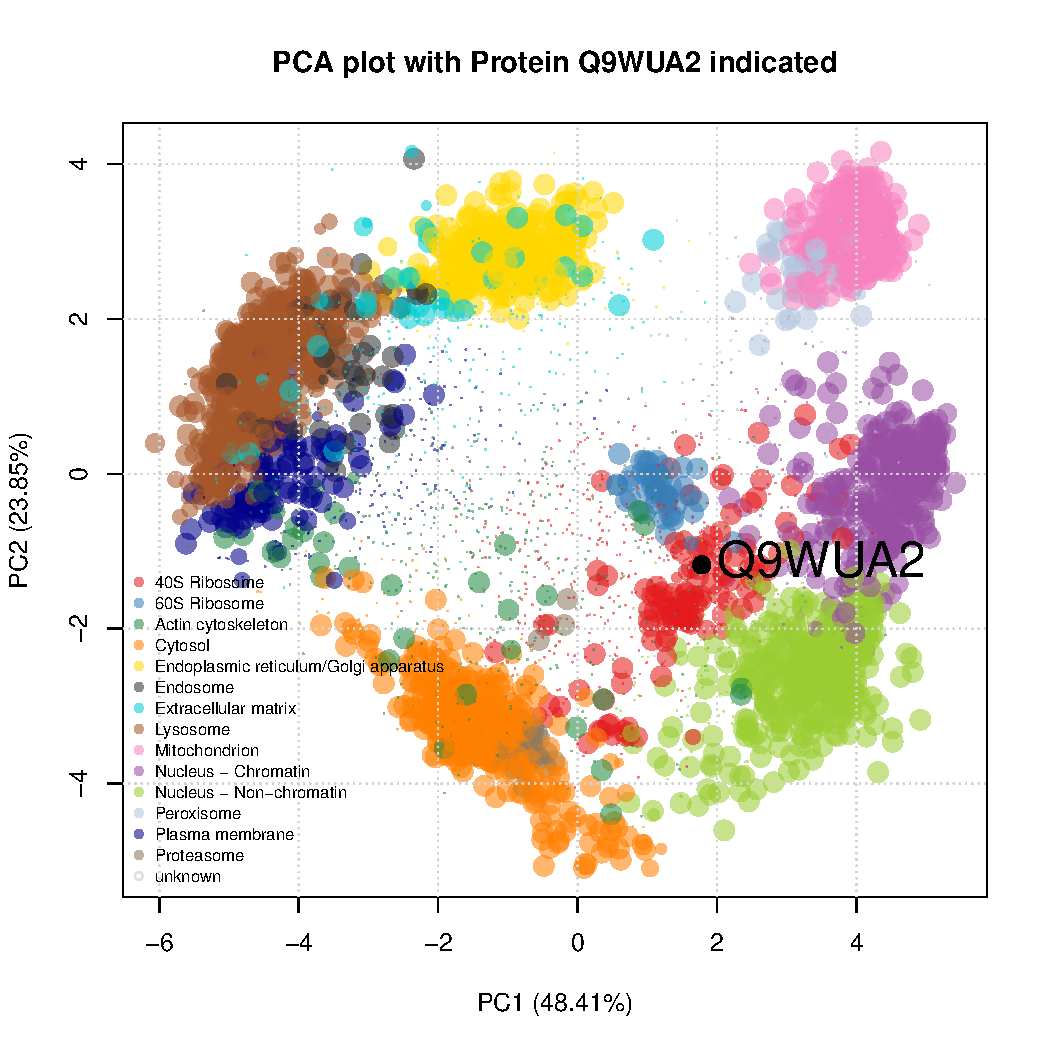
\includegraphics[width=\maxwidth]{figure/unnamed-chunk-19-1} 

}



\end{knitrout}
    \caption{}
  \end{subfigure}

  \caption{Phenylalanine-tRNA ligase beta subunit protein (Q9WUA2)
    showing localisation to the 40S Ribosome with some uncertainty
    about association to the nucleus non-chromatin.  (a) The violin
    plot shows uncertain localisation between these two sub-cellular
    localisations. (b) The quantitative profile of this protein shows
    mixed profile between the profiles of the organelle markers. (c)
    The density plot shows a complex distribution over localisations
    for this protein. (d) The protein Q9WUA2 has steady state
    distribution skewed towards the 40S Ribosome and close to the
    nucleus non-chromatin.}
  \label{fig:Q9WUA2}
\end{figure}

\begin{figure}[h]
  \centering
  \begin{subfigure}[t]{0.5\textwidth}
    \centering
\begin{knitrout}
\definecolor{shadecolor}{rgb}{0.969, 0.969, 0.969}\color{fgcolor}

{\centering 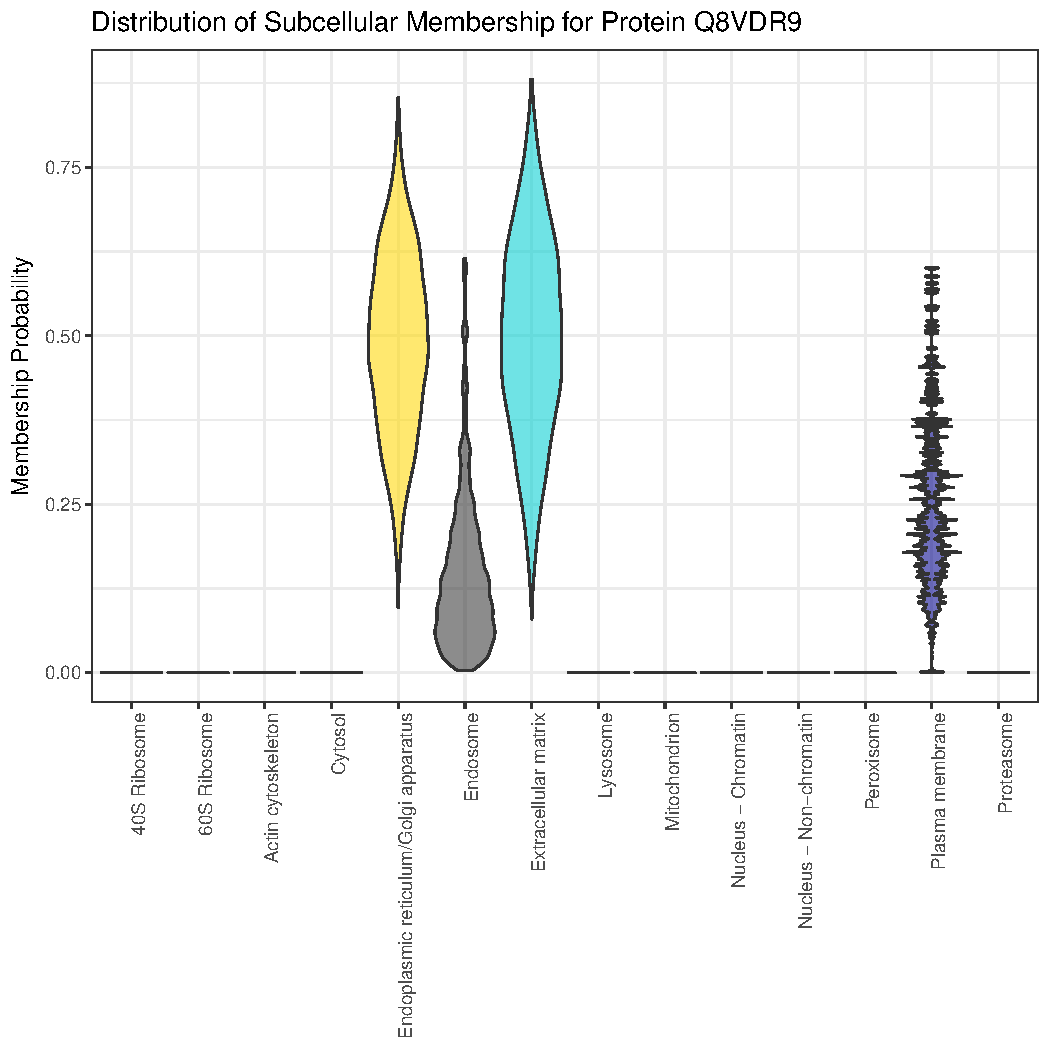
\includegraphics[width=\maxwidth]{figure/unnamed-chunk-20-1} 

}



\end{knitrout}
    \caption{}
  \end{subfigure}%
  \begin{subfigure}[t]{0.5\textwidth}
    \centering
\begin{knitrout}
\definecolor{shadecolor}{rgb}{0.969, 0.969, 0.969}\color{fgcolor}

{\centering 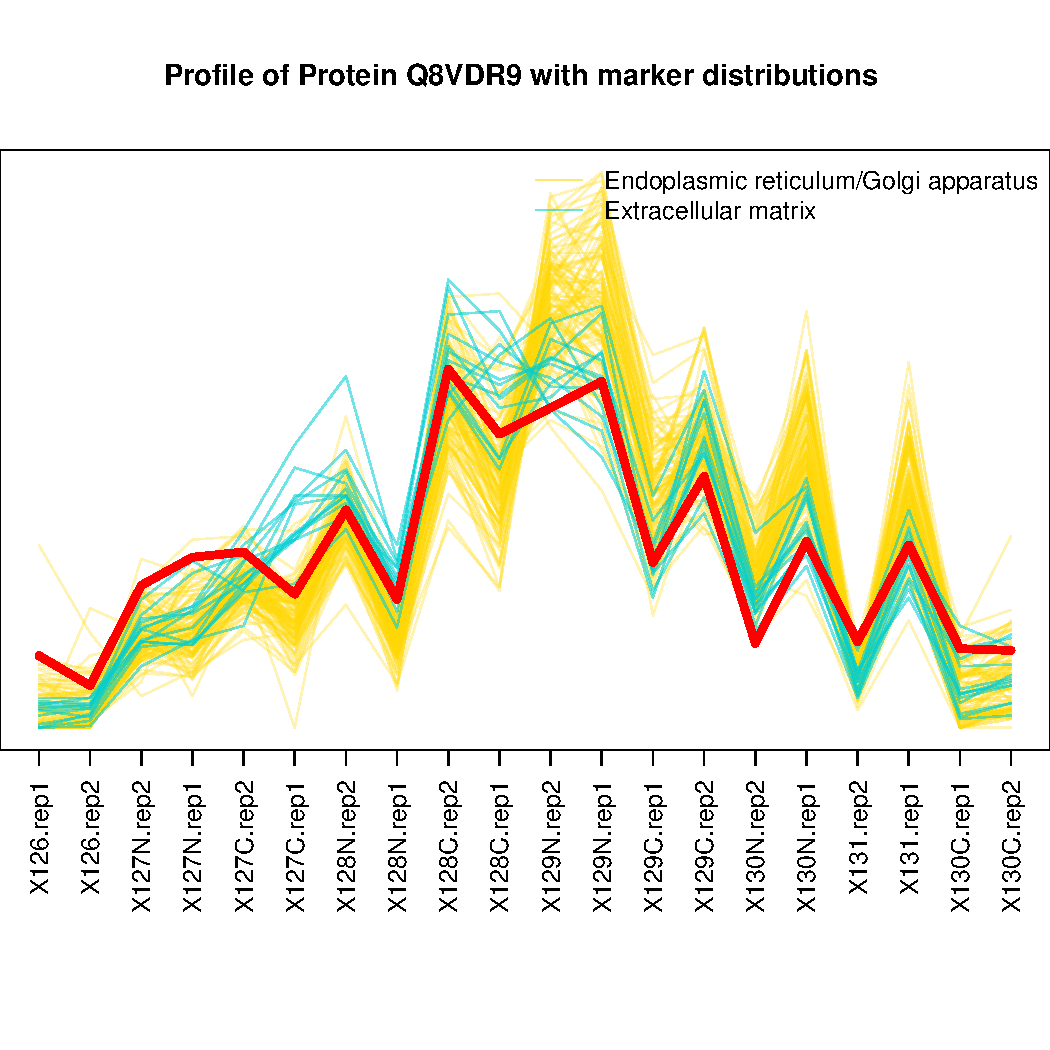
\includegraphics[width=\maxwidth]{figure/unnamed-chunk-21-1} 

}



\end{knitrout}
    \caption{}
  \end{subfigure}
  \vspace{1cm}
  \begin{subfigure}[t]{0.5\textwidth}
    \centering
\begin{knitrout}
\definecolor{shadecolor}{rgb}{0.969, 0.969, 0.969}\color{fgcolor}

{\centering 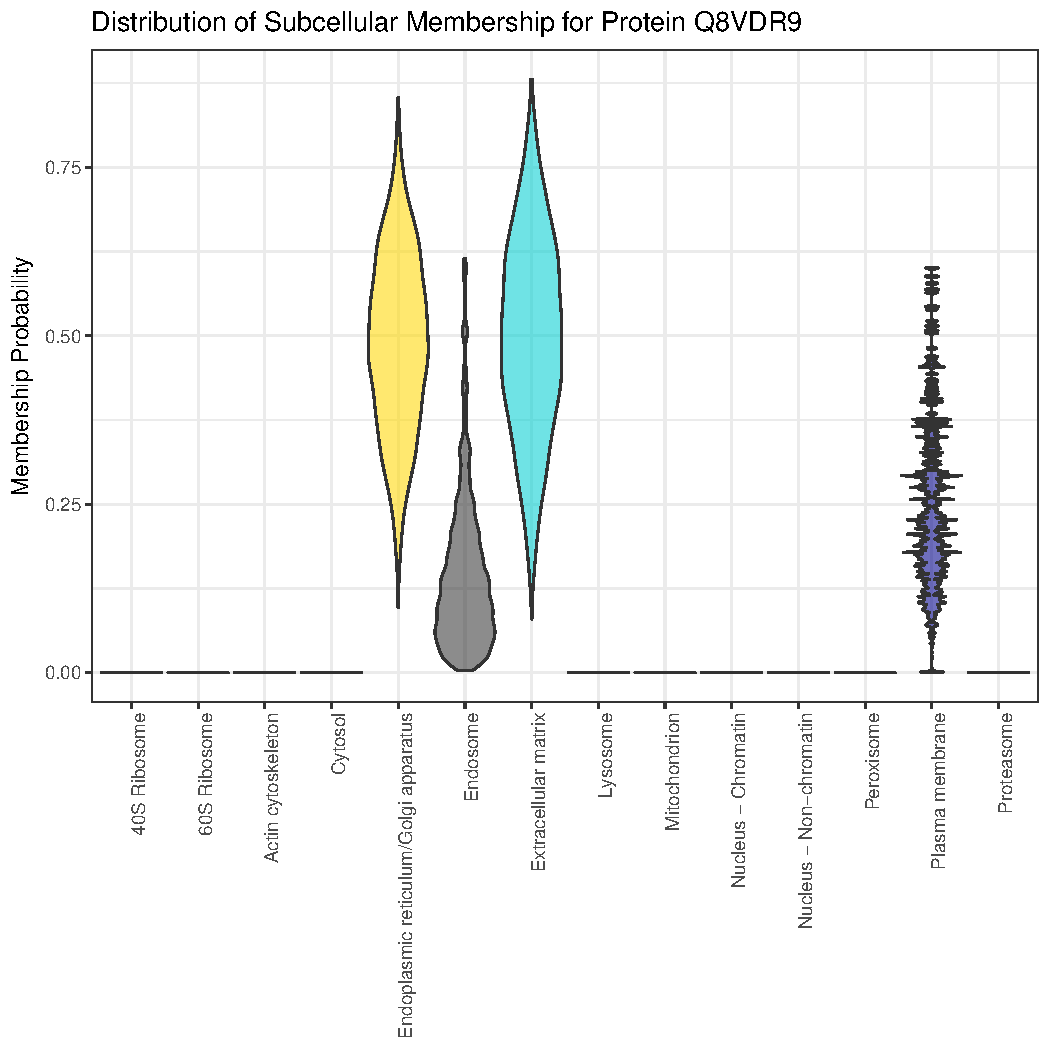
\includegraphics[width=\maxwidth]{figure/unnamed-chunk-22-1} 

}



\end{knitrout}
    \caption{}
  \end{subfigure}%
  \begin{subfigure}[t]{0.5\textwidth}
    \centering
\begin{knitrout}
\definecolor{shadecolor}{rgb}{0.969, 0.969, 0.969}\color{fgcolor}

{\centering 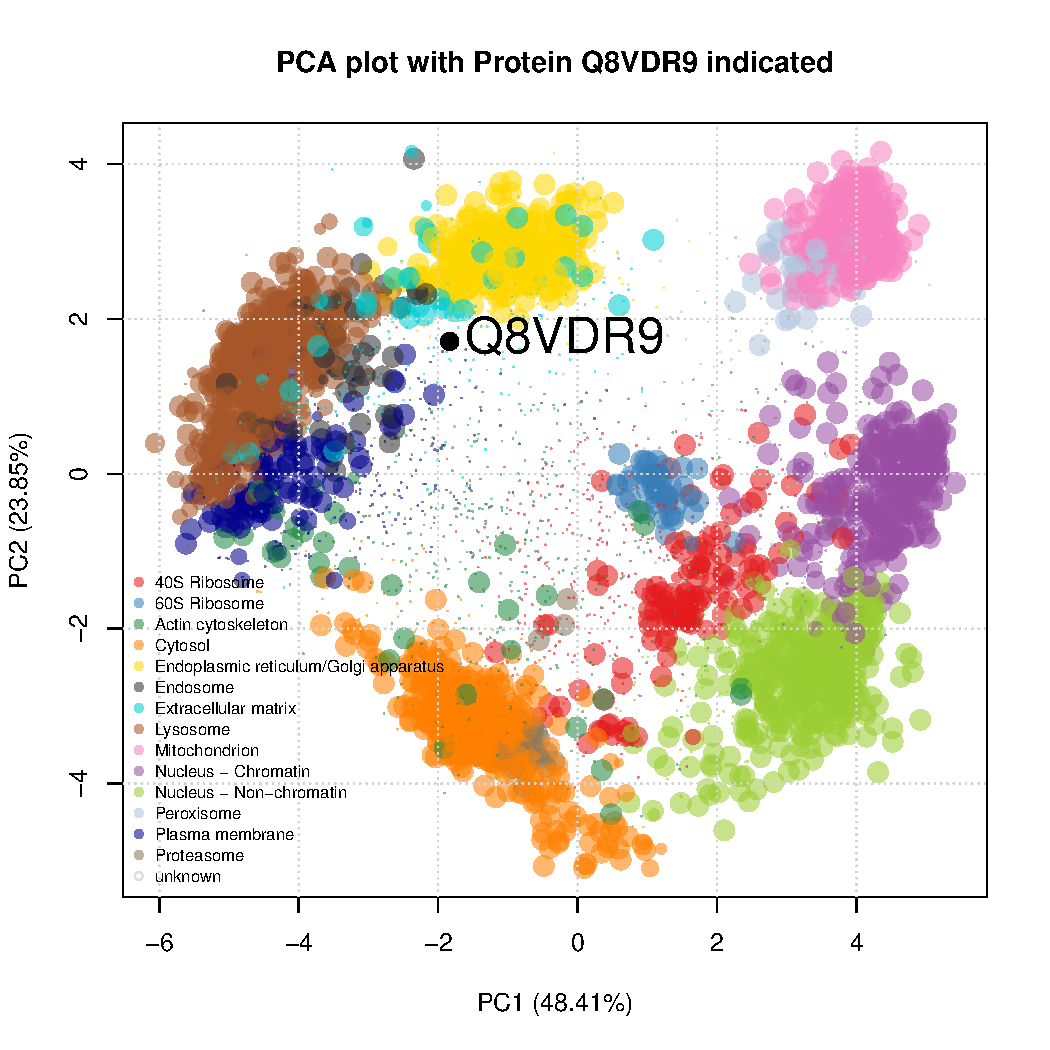
\includegraphics[width=\maxwidth]{figure/unnamed-chunk-23-1} 

}



\end{knitrout}
    \caption{}
  \end{subfigure}

  \caption{Q8VDR9 showing localisation to the outlier component.  (a)
    The violin plot shows uncertain localisation between several
    sub-cellular niches. (b) The quantitative profile of this protein
    shows mixed profile between the profiles of the organelle
    markers. (c) The density plot shows a similar localisation
    probabilities for both the ER/Golgi and Extracellular matrix. (d)
    The protein Q8VDR9 has steady state distribution in the centre of
    the plot skewed toward the secretory pathway; in particular, the
    ER/Golgi and Extracellular matrix components.}
  \label{fig:Q8VDR9}
\end{figure}



\clearpage

\subsection{Visualising whole sub-cellular proteome uncertainty}

The advantage of the TAGM is its ability to provide proteome wide
uncertainy quantification. Regions where organelle assignments overlap
are areas were uncertainty is expected to be the greatest, as well
as areas with no dominant component. We take an information
theoretic approach to summarising uncertainty in protein localisation by computing
the Shannon entropy \citep{shannon:1948} for each Monte-Carlo sample $t = 1,...,T$ of
the posterior localisation probabilities of each protein

\begin{equation}
\left\{H^{(t)} = - \sum_{k=1}^Kp^{(t)}_{ik} \log\left(p^{(t)}_{ik}\right)\right\}^{T}_{t=1},
\end{equation}

where $p^{(t)}_{ik}$ denotes the posterior localisation probabilty of
protein $i$ to component $k$ at iteration $t$. We then summarise this
as a Monte-Carlo averaged Shannon entropy.  The greater the Shannon
entropy the more uncertainty associated with the assignment of this
protein. The lower the Shannon entropy the lower the uncertainty
associated with the assignment of this protein.  In figure
\ref{figure:proteomeuncertainty} panel(a), we visualise the Shannon
entropy of each protein in a PCA plot, by scaling the pointers in
accordance to this metric. We also note that while localisation
probability (of a protein to its most probable location) and the
Shannon entropy are correlated, figure
\ref{figure:proteomeuncertainty} panel(c), it is not perfect. Thus it
is important to use both the localisation probabilities and the
uncertainty in these assignments to make conclusions.

\begin{figure}[h]
  \centering
  \begin{subfigure}[t]{0.5\textwidth}
    \centering
\begin{knitrout}
\definecolor{shadecolor}{rgb}{0.969, 0.969, 0.969}\color{fgcolor}

{\centering 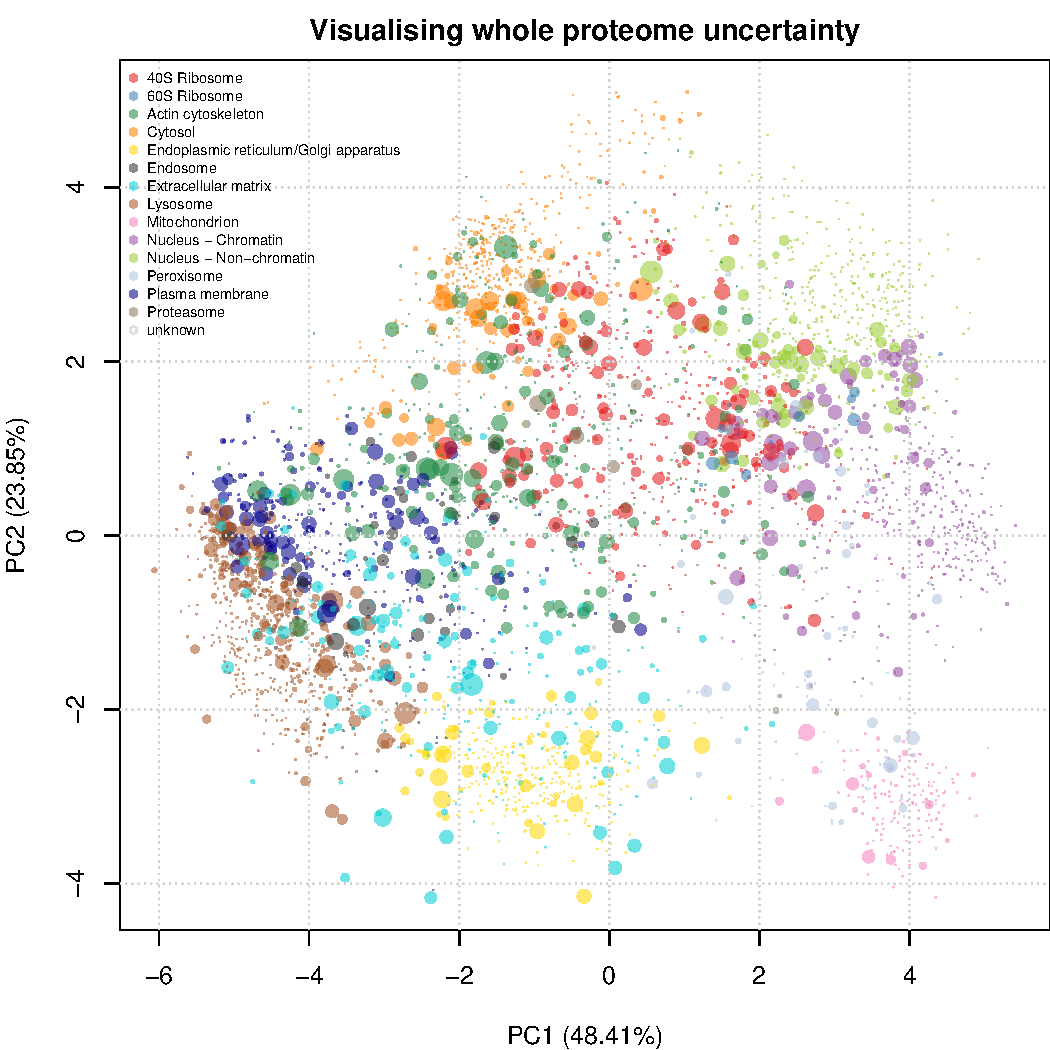
\includegraphics[width=\maxwidth]{figure/unnamed-chunk-24-1} 

}



\end{knitrout}
    \caption{}
  \end{subfigure}%
~
  \begin{subfigure}[t]{0.5\textwidth}
    \centering
\begin{knitrout}
\definecolor{shadecolor}{rgb}{0.969, 0.969, 0.969}\color{fgcolor}

{\centering 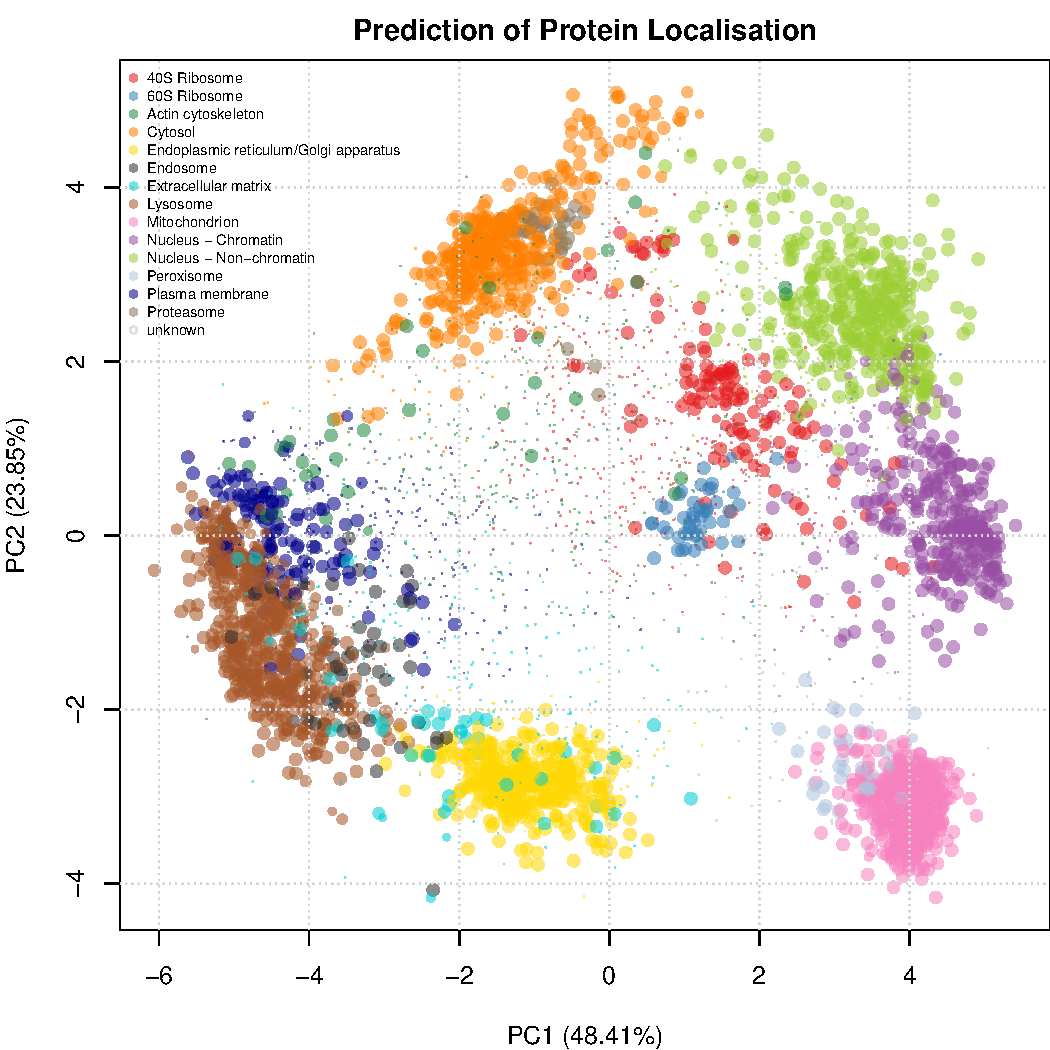
\includegraphics[width=\maxwidth]{figure/unnamed-chunk-25-1} 

}



\end{knitrout}
    \caption{}
  \end{subfigure}%
\\
  \begin{subfigure}[t]{0.5\textwidth}
    \centering
\begin{knitrout}
\definecolor{shadecolor}{rgb}{0.969, 0.969, 0.969}\color{fgcolor}

{\centering 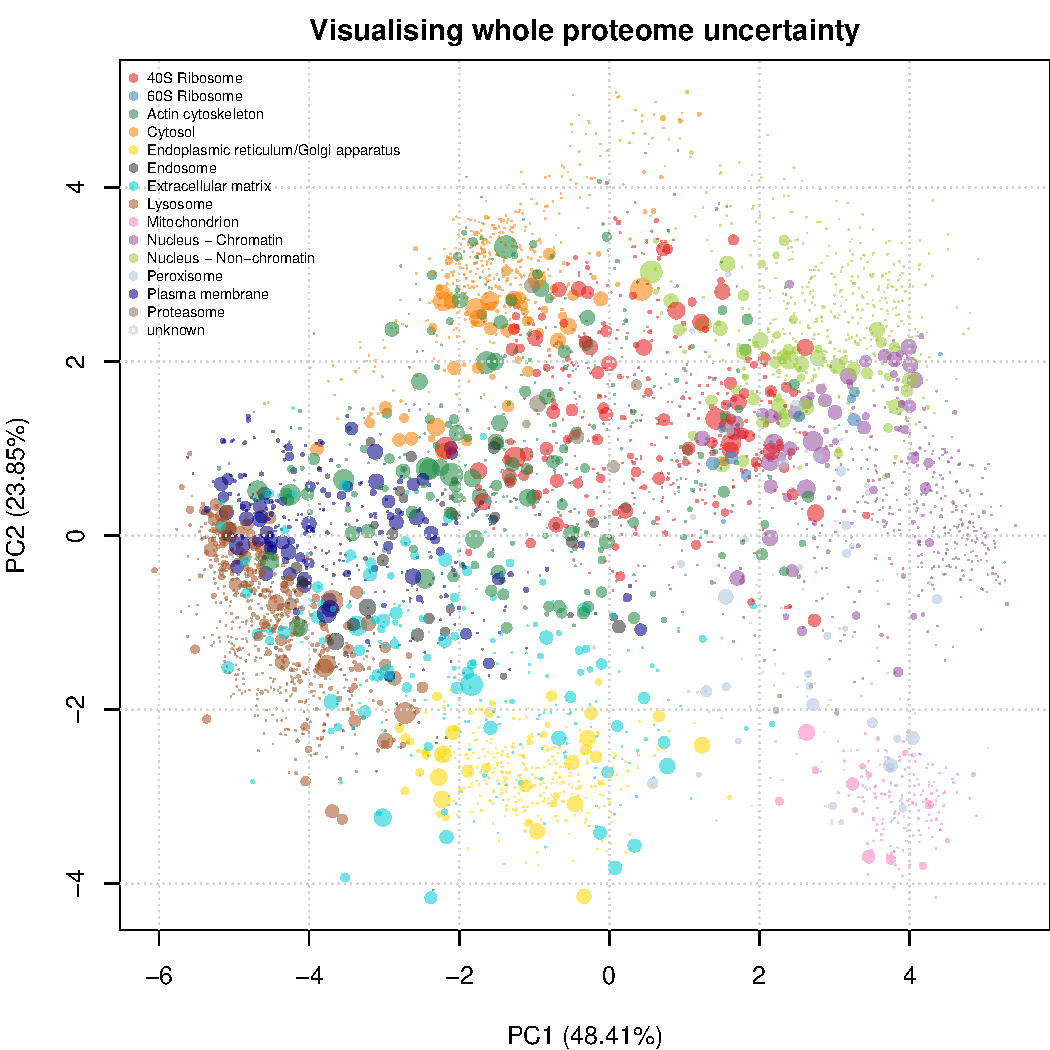
\includegraphics[width=\maxwidth]{figure/unnamed-chunk-26-1} 

}



\end{knitrout}
    \caption{}
  \end{subfigure}

  \caption{PCA plots of the mouse pluripotent embryonic stem cell data, where
    each point represents a protein and is coloured
    to its (probabilistically-)assigned organelle. (a) In this plot, the pointer is
    scaled to the Shannon entropy of this protein, with
    larger pointers indicating greater uncertainty.
    (b) In this plot, the pointer is scaled to the probability
    of that protein belonging to its assigned organelle. (c) We plot
    the localisation probabilities against the Shannon entropy
    with each protein.}
  \label{figure:proteomeuncertainty}
 \end{figure}

 Figure \ref{figure:proteomeuncertainty} demonstrates that the regions
 of highest uncertainty are those in regions where organelles
 assignments overlap. The conclusions from this plot are
 manifold. Firstly, many proteins are assigned unambiguously to
 sub-cellular localisations; that is, not only are some proteins
 assigned to organelles with high probability but also with low
 uncertainty. Secondly, there are well defined regions with high
 uncertainty, for example proteins in the secretory pathway or
 proteins on the boundary between cytosol and proteasome. Finally,
 some organelles, such as the mitochondria, are extremely well
 resolved. This observed uncertainty in the secretory pathway and
 cytosol could be attributed to the dynamic nature of these parts of
 the cell with numerous examples of proteins that traffic in and out
 of these sub-cellular compartments as part of their biological
 role. Moreover, the organelles of the secretory pathway share similar
 and overlapping physical properties making their separation from one
 another using biochemical fractionation more challenging.
 Furthermore, there is a region located in the centre of the plot
 where proteins simultaneously have low probability of belonging to
 any organelle and high uncertainty in their localisation probability.
 This suggests that these proteins are poorly described by any single
 location. These proteins could belong to multiple locations or belong
 to undescribed sub-cellular compartments. The information displayed
 in these plots and the conclusion therein would be extremely
 challenging to obtain without the use of Bayesian methodology.


\clearpage
\section{Discussion}

We have demonstrated that a Bayesian framework, based on Gaussian
mixture models, for spatial proteomics can provide whole sub-cellular
proteome uncertainty quantification on the assignment of proteins to
organelles and such information is invaluable. Performing MAP
inference using our generative model provides fast and straightforward
approach, which is vital for quality control and early data
exploration. Full posterior inference using MCMC provides not only
point estimates of the posterior probability that a protein belongs to
a particular sub-cellular niche, but uncertainty in this
assignment. Then, this uncertainty can be summarised in several ways,
including, but not limited to, equi-tailed credible intervals of the
Monte-Carlo samples of posterior localisation probabilities.
Posterior distributions for indivdual proteins can then be rigorously
interrogated to shed light on their biological mechanisms; such as,
transport, signalling and interactions.

As well as the local uncertainty seen by exploring individual
proteins, we further explored using a Monte-Carlo averaged Shannon
entropy to visualise global uncertainty. Regions of high uncertainty,
as measured using this Shannon entropy, reflect highly dynamics
regions of the sub-cellular environment.  Hence, biologists can now
explore uncertainty at different levels and then are able to make
quantifiable conclusions and insights about their data.  Furthermore,
our Bayesian model is interpretable and our inferences are fully
conditional on our data, allowing them to be easily modified with
changing experimental design.

In addition, we produced competitive classifier performance to the
state-of-the-art classifiers. We considered two traditional
machine-learning methods: the SVM and KNN classifiers; as well as two
classifiers based on our model: a MAP classifier and classification
based on MCMC. We compared all methods on 19 different spatial
proteomics datasets, across four different organisms. When considering
the macro-F1 score as a performace metric, no single classifier
outperformed another across all datasets. However, using MCMC based
inference our method significantly outperforms the SVM and KNN
classifiers with respect to the quadratic loss in $16$ our of $19$
datasets. This allows us to have greater confidence in our conclusions
when they are draw from our Bayesian inferences. Furthermore, using
MCMC provides a wealth of additional information, and so becomes the
mothod of choice for analysing spatial proteomics data.

Analysis of a \textit{hyper}LOPIT experiment applied to mouse
pluripotent embryonic stem cells demonstrated that the additional
layer of information that our model provides is biologically
relevant and provides further avenues for additional
exploration. Moreover, applying our method to a biologically
significant dataset now provides the scientific community with
localisation information on up to 4,000 proteins for the mouse
pluripotent stem cell proteome. Figure \ref{figure:ConcludePlot}
demonstrates that from an initial input of roughly 1,000 marker
proteins with \textit{a priori} known location and 4,000 unknown
proteins with unknown location, both methods can provide rigorous
localisation information on roughly 2,000 proteins. However, our
methodology, by also considering uncertainty, allows us to obtain
information on another 1,000 proteins.  Thus, we have augmented this
dataset by providing uncertainty quantification on the localisation of
proteins to their sub-cellular niches, which had been previously
unavailable.

We have also provided a new set of visualisation methods to accompany
our model, which allow us to easily interrogate our data. High quality
visualisation tools are essential for rigorous quality control and
sound biological conclusions.  Our methods have been developed in the
R statistical programming language and we continue to contribute to
the Bioconductor project \citep{Bioconductor::2004, Huber::2015} with
inclusion of our methods within the pRoloc package
\citep{pRoloc:2014}. The underlying source code used to generate this
document is available at
\url{https://github.com/lgatto/2018-TAGM-paper}.

Currently, our model cannot integrate localisation information from
different data sources nor can it explicity model proteins with
multiple localisation. In addition, extensions to semi-supervised
methods are under consideration to detect novel sub-cellular
niches. These are the subjects of further work.

\begin{figure}[h]

\centering
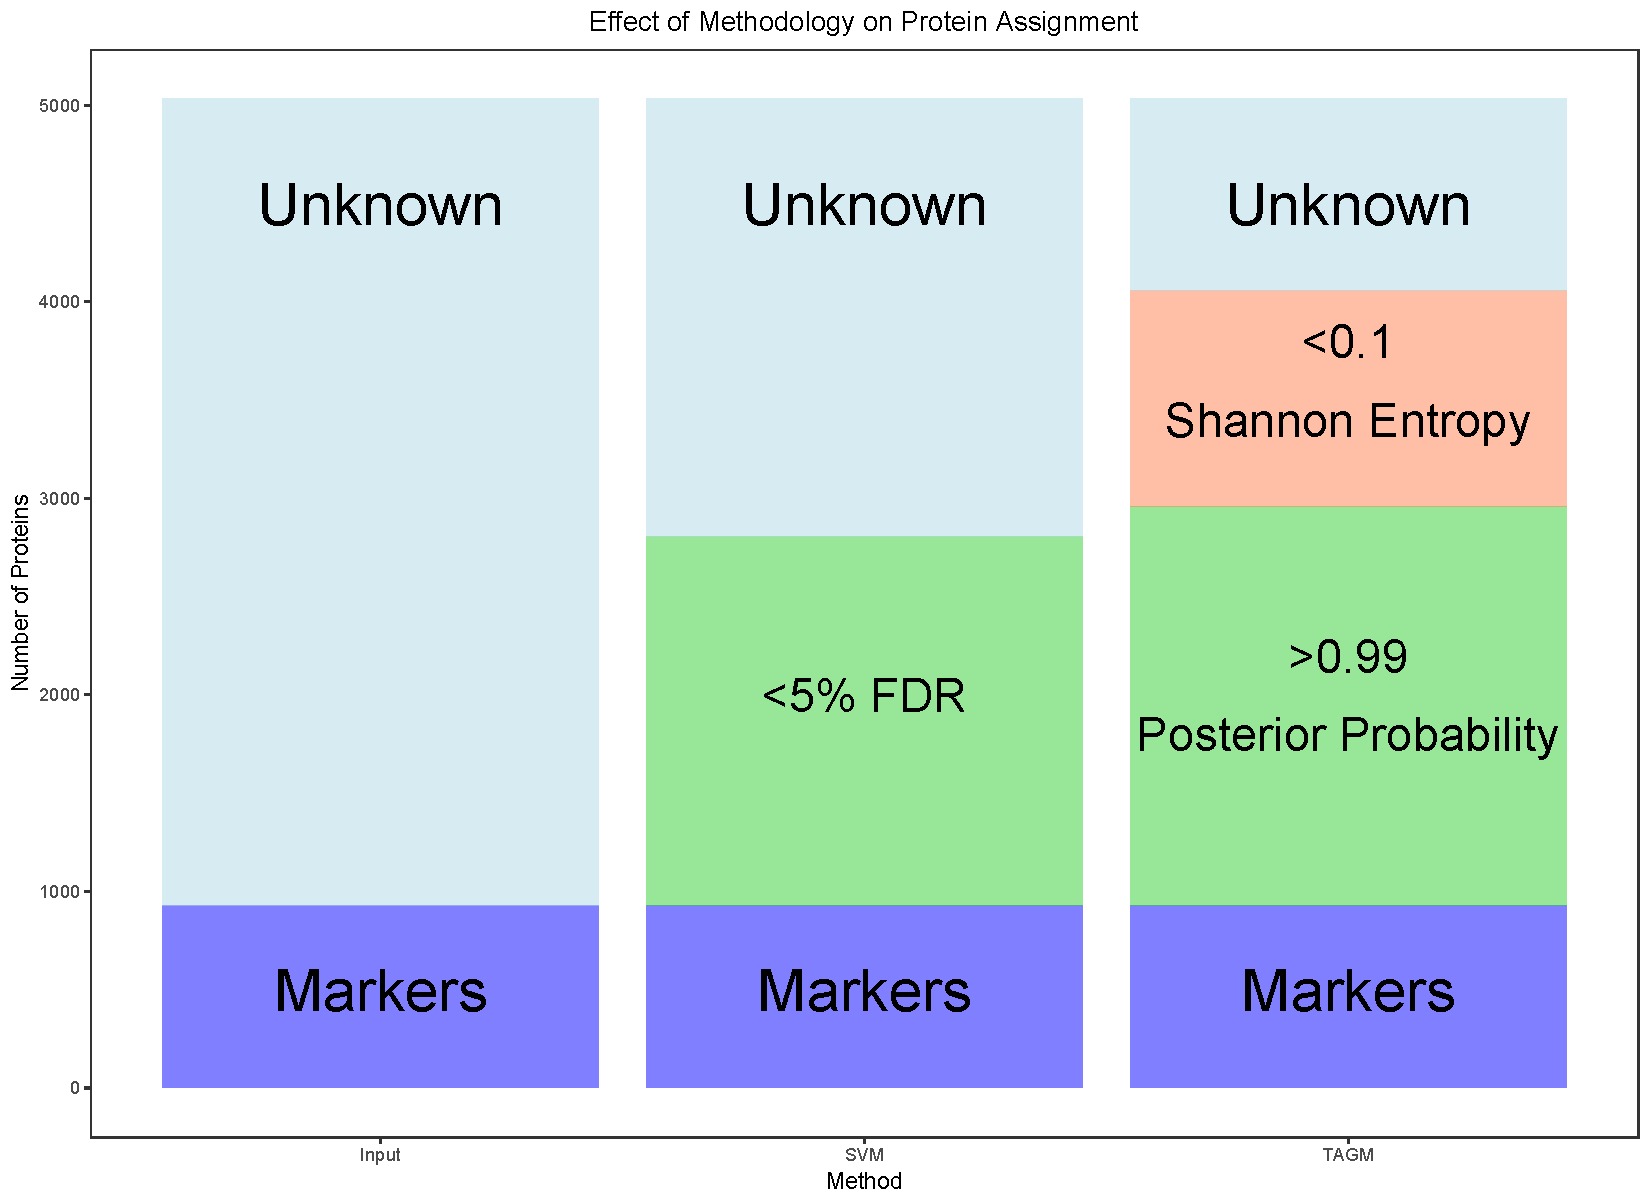
\includegraphics[width=.7\textwidth]{ConcludePlot.pdf}
\caption{The barplot demonstrates the effect of applying different
  methodologies on protein assignment when applied the mouse
  pluripotent embryonic stem cell data. Roughly 2000 proteins are
  classified using either methodology; however, TAGM can draw
  additional conclusions about an extra 1000 proteins by quantifying
  uncertainty.}
\label{figure:ConcludePlot}
\end{figure}


\bigskip

\section{Model and methods}\label{section:methods}

We describe in this section the probabilistic model that uses the
labelled data to associate un-annotated proteins to specific
organelles or sub-cellular compartments.

\subsection{Mixture models for spatial proteomic data}

We observe $N$ protein profiles each of length $L$, corresponding to
the number of quantified fractions along the gradient density,
including combining replicates.  For $i = 1, \ldots, N$, we denote the
profile of the $i$-th protein by
${\bf x}_i = [x_{1i}, \ldots, x_{Li}]$.  We suppose that there are $K$
known sub-cellular compartments to which each protein could localise
(e.g. cytoplasm, endoplasmic reticulum, mitochondria, \ldots).
Henceforth, we refer to these $K$ sub-cellular compartments as {\em
  components}, and introduce component labels $z_i$, so that $z_i = k$
if the $i$-th protein localises to the $k$-th component. We denote by
$X_L$ the set of proteins whose component labels are known, and by
$X_U$ the set of unlabelled proteins.  If protein $i$ is in $X_U$, we
desire the probability that $z_i = k$ for each $k = 1, \ldots, K$.
That is, for each unlabelled protein, we want the probability of
belonging to each component (given a model and the observed data).


We initially model the distribution of profiles associated with
proteins that localise to the $k$-th component as multivariate normal
with mean vector $\boldsymbol{\mu}_k$ and covariance matrix
$\Sigma_k$, so that:

\begin{align}
{\bf x}_i | z_i = k \quad \sim \mathcal{N}(\boldsymbol{\mu}_k, \Sigma_k). \label{equation::preq}
\end{align}

For any $i$, we define the prior probability of the $i$-th protein
localising to the $k$-th component to be $p(z_i = k) = \pi_k$.
Letting
$\boldsymbol{\theta} = \{\boldsymbol{\mu}_k, \Sigma_k \}_{k = 1}^K$
denote the set of all component mean and covariance parameters, and
$\boldsymbol{\pi} = \{\pi_k\}_{k = 1}^K$ denote the set of all mixture
weights, it follows (from the law of total probability) that:

\begin{align}
p({\bf x}_i | \boldsymbol{\theta}, \boldsymbol{\pi} ) = \sum_{k = 1}^K \pi_k f({\bf x}_i|\boldsymbol{\mu}_k, \Sigma_k),\label{equation::mmeq}
\end{align}

where $f({\bf x} | \boldsymbol{\mu}, \Sigma)$ denotes the density of
the multivariate normal with mean vector $\boldsymbol{\mu}$ and
covariance matrix $\Sigma$ evaluated at ${\bf x}$.

Equation \eqref{equation::mmeq} defines a generative probabilistic
model known as a {\em mixture model}.  Such models are useful for
describing populations that are composed of a number of distinct
homogeneous subpopulations.  In our case, we model the full complement
of measured proteins as being composed of $K$ subpopulations, each
corresponding to a different organelle or sub-cellular
compartment. The literature of mixture model applications to biology
is rich and some recent example include applications to retroviral
integration sites \citep{Kirk:2016}, genome-wide associations studies
\citep{Liley:2017} and single-cell transcriptomics
\citep{Lonnberg:2017}.

Though some proteins are well described as belonging to a single
component, many proteins multi-localise or might belong to
uncharacterised organelles. In order to allow the model to better
account for these "outliers" that cannot be straightforwardly
allocated to any single known component, we extend it by introducing
an additional "outlier component". To do this, we augment our model by
introducing a further indicator latent variable $\phi$. Each protein
${\bf x}_i$ is now described by an additional variable $\phi_i$, with
$\phi_i = 1$ indicating that protein ${\bf x}_i$ belongs to a
organelle derived component and $\phi_i = 0$ indicating that protein
${\bf x}_i$ is not well described by these known components. This
outlier component is modelled as a multivariate T distribution with
degrees of freedom $\kappa$, mean vector $\bf{M}$, and scale matrix
$V$. Thus equation \eqref{equation::preq} becomes

\begin{align}
{\bf x}_i | z_i = k, \phi_i \quad \sim \mathcal{N}(\boldsymbol{\mu}_k, \Sigma_k)^{\phi_i}\mathcal{T}(\kappa, \boldsymbol{M}, V)^{1 - \phi_i }.
\end{align}

Further let $g({\bf x | \kappa, \bf{M}, V} )$ denote the density of
the multivariate T-distribution so that Equation
\eqref{equation::mmeq} becomes:

\begin{equation} \label{equation::tammeq}
  \begin{split}
    p({\bf x}_i| \boldsymbol{\theta}, \boldsymbol{\pi} ,\phi_i, \kappa, {\bf M}, V) &=  \sum_{k=1}^{K}\pi_k\left(f({\bf x}_i|\boldsymbol{\mu}_k, \Sigma_k)^{\phi_i}g({\bf x}_i|\kappa, \boldsymbol{M}, V)^{1 - \phi_i }\right).\\
  \end{split}
\end{equation}

For any $i$, we define the prior probability of the $i$-th protein
belonging to the outlier component as $p(\phi_i = 0) = \epsilon$.

We can then rewrite equation \eqref{equation::tammeq} in the following way:

\begin{equation}\label{equation::tammepseq}
  \begin{split}
    p({\bf x}_i| \boldsymbol{\theta}, \boldsymbol{\pi} , \kappa, \epsilon, {\bf M}, V) &=  \sum_{k=1}^{K}\pi_k\left((1-\epsilon)(f({\bf x}_i |\boldsymbol{\mu}_k, \Sigma_k) + \epsilon g({\bf x}_i|\kappa, \boldsymbol{M}, V)\right),\\
  \end{split}
\end{equation}

Throughout we take $\kappa = 4$, ${\bf M}$ as the global mean, and $V$
as half the global variance of the data. The reason for formulating
the model as in equation \eqref{equation::tammeq} is because it leads
to a flexible modelling framework. Furthermore, $\phi$ has an elegant
model selection interpretation, since it decides whether ${\bf x}_i$
is better modelled by the known components or the outlier component.
It is important to note that $f$ and $g$ could be replaced by many
combinations of distributions and thus could be valuable in modelling
other datasets. The choice of parameters for the multivariate
T-distribution was decided so that it mimicked a multivariate normal
component with the same mean and variance but with heavier tails to
better capture dispersed proteins, which we refer to as outlier
proteins throughout the text.  Similar approaches for modelling
outliers have been explored in the literature and often the outlier
term is considered constant or as a Poisson process, independent of
the observation \citep{Banfield::1993, Cooke::2011, Coretto::2016,
  Hennig::2004}.


\subsection{Model fitting}

We adopt a Bayesian approach toward inferring the unknown parameters,
$\boldsymbol{\theta} = \{\boldsymbol{\mu}_k, \Sigma_k \}_{k = 1}^K$,
$\boldsymbol{\pi} = \{\pi_k\}_{k = 1}^K$, and $\epsilon$ of the
mixture model presented in Equation \eqref{equation::tammeq}.  For
$\boldsymbol{\pi}$, we take a conjugate symmetric Dirichlet prior with
parameter~$\beta$, so that
$\pi_1, \ldots, \pi_K \sim \mbox{Dirichlet}(\beta)$; and for the
component-specific parameters $\boldsymbol{\mu}_k$ and $\Sigma_k$ we
take conjugate normal-inverse-Wishart (NIW) priors with parameters
$\{\boldsymbol{\mu}_0, \lambda_0, \nu_0, S_0\}$, so that:

\begin{equation} \label{equation::prior}
  \mu_k, \Sigma_k \quad \sim \mathcal{N}\left(\boldsymbol{\mu}_k|\boldsymbol{\mu}_0, \frac{\Sigma_{k}}{\lambda_0}\right)I\mathcal{W}\left(\Sigma_{k}|\nu_0, S_0\right).
\end{equation}

We also place a conjugate Beta prior on $\epsilon$ with parameters $u$
and $v$, so that $\epsilon \sim \mathcal{B}(u,v)$.  Allowing
$\epsilon$ to be random allows us to infer the number of proteins that
are better described by an outlier component rather than any known
component.

The full model, which we henceforth refer to as a T-augmented Gaussian
Mixture model (TAGM), can then be summarised by the plate diagram
shown in Figure \ref{plateDiagram}.

\begin{figure}[H]
  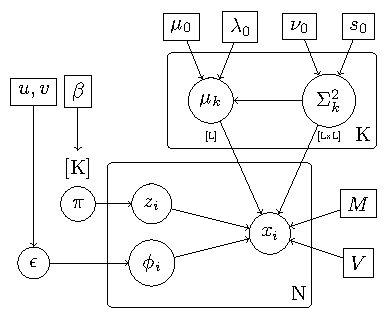
\includegraphics[width=8cm]{graphmodel2.pdf}
  \centering
  \caption{Plate diagram for TAGM model. This diagram specifies the
    conditional independencies and parameters in our
    model.}\label{plateDiagram}
\end{figure}

To perform inference for the parameters, we make use of both the
labelled and unlabelled data. For the labelled data $X_L$, since $z_i$
and $\phi_i$ are known for these proteins, we can update the
parameters with their data analytically by exploiting conjugacy of the
priors \citep[see, for example,][]{Gelman:1995}. For the unlabelled
data we do not have such information and so in the next sections we
explain how to make inferences of the latent variables.

\subsection{Prediction of localisation of unlabelled proteins}

Having obtained the posterior distribution of the model parameters
analytically using, at first, the labelled data only, we wish to
predict the component to which each of the unlabelled proteins
belongs. The probability that a protein belongs to any of the $K$
known components, that is $z_i = k$ and $\phi_i = 1$, is given by (see
appendix \ref{apd:EMderv} for derivations):

\begin{equation}\label{equation::estep1}
\begin{split}
p(\phi_i = 1, z_i = k|{\bf x}_i, \boldsymbol{\theta}, \boldsymbol{\pi} , \epsilon,\kappa, {\bf M}, V)  & = \frac{\pi_k(1-\epsilon)f({\bf x}_i|\boldsymbol{\mu}_k, \Sigma_{k})}{\sum_{k=1}^{K}\pi_k\left((1-\epsilon) f({\bf x}_i|\boldsymbol{\mu}_k, \Sigma_k) + \epsilon g({\bf x}_i|\kappa, {\bf M}, V)\right)},
\end{split}
\end{equation}
whilst on the other hand,
\begin{equation}\label{equation::estep2}
\begin{split}
p(\phi_i = 0, z_i = k|{\bf x}_i, \boldsymbol{\theta}, \boldsymbol{\pi},\kappa, \epsilon, {\bf M}, V)  = \frac{\pi_k \epsilon g({\bf x}_i|\kappa, {\bf M}, V)}{\sum_{k=1}^{K}\pi_k\left((1-\epsilon) f({\bf x}_i|\boldsymbol{\mu}_k, \Sigma_k) + \epsilon g({\bf x}_i|\kappa, {\bf M}, V)\right)}.
\end{split}
\end{equation}

Processing of the unlabelled data can be done by inferring {\em maximum
  a posteriori} (MAP) estimates for the parameters. However, this
approach fails to account for the uncertainty in the parameters, thus
we additionally explore inferring the distribution over these
parameters.

\subsubsection{Maximum a posteriori prediction}

We use the Expectation-Maximisation (EM) algorithm \citep{EM:1977} to
find {\em maximum a posteriori} (MAP) estimates for the parameters
\cite[see, for example,][]{Murphy:2012}. To specify the parameters of
the prior distributions, we use a simple set of heuristics provided by
\cite{Fraley:2007}. By defining the following quantities

\begin{equation}\label{equation::estepfinal}
\begin{split}
a_{ik} = & p(z_i = k, \phi_i = 1|{\bf x}_i), b_{ik} = p(z_i = k, \phi_i = 0|{\bf x}_i) \\
w_{ik} = & p(z_i = k|x_i) = a_{ik} + b_{ik}\\
a_k = & \sum_{i=1}^{n}a_{ik}, a = \sum_{k=1}^{K}a_k \\
b_k = & \sum_{i=1}^{n}b_{ik}, b = \sum_{k=1}^{K}b_k \\
r_k = & \sum_{i=1}^{n}w_{ik},
\end{split}
\end{equation}

we can compute

\begin{equation}\label{equation::Posterior}
\begin{split}
\lambda_k = &\lambda_0 + a_k, \\
\nu_k = & \nu_0 + a_k, \\
m_k = & \frac{a_k\bar{\boldsymbol{x}}_k + \lambda_0\mu_0}{\lambda_k},\\
S_k^{-1}  = & S_0^{-1} + \frac{\lambda_0 a_k}{\lambda_k}(\bar{\boldsymbol{x}}_k - \mu_0)^{T} (\bar{\boldsymbol{x}}_k - \mu_0) + \sum_{i=1}^{n} a_{ik}(x_i -\bar{\boldsymbol{x}}_k)^{T}(x_i -\bar{\boldsymbol{x}}_k).
\end{split}
\end{equation}

Then the parameters of the posterior mode are:

\begin{equation}\label{equation::MAP}
\begin{split}
\hat{{\bf\mu}}_k = &m_k \\
\hat{\Sigma}_k = &\frac{1}{\nu_k + D + 2}S_k^{-1}.
\end{split}
\end{equation}

We note if $\boldsymbol{x}_i$ is a labelled protein then $a_{ik} = 1$
and these parameters can be updated without difficulty.  The above
equation constitutes a backbone of the E-step of the EM algorithm, with
the entire algorithm specified by the following summary:


E-Step: Given the current parameters compute the values given by
equations (\ref{equation::estepfinal}), with formulae provided in
equations (\ref{equation::estep1}) and (\ref{equation::estep2}).

\bigskip

M-Step: Compute
\[\epsilon = \frac{ u + b - 1}{(a+b) + (u+v) - 2},\]
and
\[\pi_k = \frac{r_k + \beta_k - 1}{N + \sum \beta_k - K},\]
as well as
\[\bar{\boldsymbol{x}}_k = \frac{1}{a_k}\left(\sum_{i=i}^{n}a_{ik}{\bf x}_i\right).\]

Finally, compute the MAP estimates given by equations
(\ref{equation::MAP}). These estimates are then used in the following
iteration of the E-step.


Denoting by Q the expected value of the log-posterior and letting $t$
denote the current iteration of the EM algorithm, we iterate until
$\lvert Q(\boldsymbol{\theta}|\boldsymbol{\theta}_{t}) -
Q(\boldsymbol{\theta}|\boldsymbol{\theta}_{t-1})\rvert < \delta$ for
some pre-specified $\delta >0$.  Once we have found MAP estimates for
the parameters $\boldsymbol{\theta}_{MAP}$, $\boldsymbol{\pi}_{MAP}$
and $\epsilon_{MAP}$ we proceed to perform prediction. We plug the MAP
parameter estimates into Equation \eqref{equation::estep1} in order to
obtain the posterior probability of protein $i$ localising to
component $k$,
$p(z_i = k, \phi = 1 | {\bf x}_i, \boldsymbol{\theta}_{MAP},
\boldsymbol{\pi}_{MAP} , \epsilon_{MAP},\kappa, {\bf M}, V)$. To make
a final assignment, we may allocate each protein according to the
component that has maximal probability.  A full technical derivation
of the EM algorithm can be found in the appendix (appendix
\ref{apd:EMderv}).

\subsubsection{Uncertainty in the posterior localisation probabilities}\label{section::MCMC}

The MAP approach described above provides us with a probabilistic
assignment,
$p(z_i = k, \phi = 1 | {\bf x}_i, \boldsymbol{\theta}_{MAP},
\boldsymbol{\pi}_{MAP} , \epsilon_{MAP},\kappa, {\bf M}, V)$, of each
unlabelled protein to each component.  However, it fails to account
for the uncertainty in the parameters $\boldsymbol{\theta}$,
$\boldsymbol{\pi}$ and $\epsilon$. To address this, we can sample
parameters from the posterior distribution.

Let
$\{\boldsymbol{\theta}^{(t)}, \boldsymbol{\pi}^{(t)},
\epsilon^{(t)}\}_{t=1}^T$ be a set of $T$ sampled values for the
parameters $\boldsymbol{\theta}$, $\boldsymbol{\pi}, \epsilon$, drawn
from the posterior.


The assignment probabilities can then be summarised by the Monte-Carlo
average:

\[p(z_i = k, \phi = 1 | {\bf x}_i, \epsilon, {\bf M}, V) \approx T^{-1}\sum_{t=1}^{T}p(z_i = k, \phi = 1 | {\bf x}_i, \boldsymbol{\theta}^{(t)}, \boldsymbol{\pi}^{(t)} , \epsilon^{(t)}, \kappa, {\bf M}, V).\]

Other summaries of the assignment probabilities can be determined in
the usual ways to obtain, for example, interval-estimates. We
summarise interval-estimates using the $95\%$ equi-tailed interval,
which is defined by the $0.025$ and $0.975$ quantiles of the
distribution of assignment probabilities,
$\{p(z_i = k, \phi = 1 | {\bf x}_i, \boldsymbol{\theta}^{(t)},
\boldsymbol{\pi}^{(t)} , \epsilon^{(t)}, {\bf M}, V) \}_{t=1}^T$.

Sampling parameter values in our model requires us to compute the
required conditional probabilities and then a straightforward Gibbs
sampler can be used to sample in turn from these conditionals. In
addition, we can bypass sampling the parameters by exploiting the
conjugacy of our priors. By marginalising parameters in our model we
can obtain an efficient collapsed Gibbs sampler and therefore only
sample the component allocation probabilities and the outlier
allocation probabilities. The derivations and required conditionals
can be found in the appendix (appendix \ref{app::gibbs}).

\subsection{Classifier assessment}\label{section::assessment}

In later sections we compare the classification performance of the two
above learning schemes to the K-nearest neighbours (KNN) and the
weighted support vector machine (SVM) classifiers.

The following schema was used to assess the classifier performance of
all methods. We split the marker sets for each experiment into a
class-stratified training $(80\%)$ and test $(20\%)$ partitions, with
the separation formed at random. The true classes of the test profiles
are withheld from the classifier, whilst the algorithm is trained. The
algorithm is then assessed on its ability to predict the classes of
the proteins in the test partition for generalisation accuracy. How
each classifier is trained is specific to that classifier.  The KNN
and SVM have hyperparameters optimised using $5$-fold
cross-validation. This $80/20$ data stratification is performed $100$
times in order to produce $100$ sets of macro-F1 \citep{He::2009}
scores and class specific F1 scores \citep{Breckels:2016}. The F1
score is the harmonic mean of the precision and recall, more
precisely:
\[\text{precision}=\frac{tp}{tp+fp}, \text{recall} = \frac{tp}{tp+fn}.\]

tp denotes the number of true positives; fp the number of
false positives and fn the number of false negatives. Thus

\[\text{F1}=2\times\frac{\text{precision}\times\text{recall}}{\text{precision}+\text{recall}}.\]

High Macro F1 scores indicates that marker proteins in the test
dataset are consistently correctly assigned by the classifier. We note
that accuracy alone is an inadequate measure of performance, since it
fails to quantify false positives.

However, a Bayesian Generative classifier produces probabilistic
assignment of observations to classes. Thus while the classifier may
make an incorrect assignment it may do so with low probability. The F1
score is unforgiving in this situation and will not use this
information.  To measure this uncertainty, we introduce the quadratic
loss which allows us to compare probabilistic assignments
\citep{Gneiting:2007}.  For the SVM, a logistic distribution is fitted
using maximum likelihood estimation to the decision values of all
binary classifiers. Then, the membership probabilities for the
multi-class classification is calculated using quadratic optimisation.
The logistic regression model assumes errors which are distributed
according to a centred Laplace distribution for the predictions, where
maximum likelihood estimation is used to estimate the scale parameter
\citep{Meyer:2017}.  For the KNN classifier, we interpret the
proportion of neighbours belonging to each class as a non-parametric
posterior probability. To avoid non-zero probabilities for classes we
perform Laplace smoothing; that is, the posterior allocation
probability is given by

\begin{equation}
p(z_i = k|x_i) = \frac{N_{ik} + \alpha d_k C}{K + \alpha C},
\end{equation}

where $N_{ik}$ is the number of neighbours belonging to class $k$ in
the neighbourhood of $x_i$, $C$ is the number of classes, $K$ is the
number of nearest neighbours (optimised through 5-fold cross
validation) and $d_k$ is the incidence rate of each class in the
training set. Finally, $\alpha >0$ is the pseudo-count smoothing
parameter. Motivated by a Bayesian interpretation of placing a
Jeffrey's type Dirichlet prior over multinomial counts, we choose
$\alpha = 0.5$ \citep{Hazimeh:2015, Valcarce:2016, Manning:2008}.  The
quadratic loss is given by the following formula:

\begin{equation}
  Q_2 = \sum_{i = 1}^{N}\lVert q_i - p_i\rVert_2^2,
\end{equation}

where $\lVert\cdot\rVert_2$ is the $l_2$ norm and $q_i$ is the true
classification vector and $p_i$ is a vector of predicted assignments
to each class. It is useful to note that the corresponding risk
function is the mean square error (MSE), which is the expected value
of the quadratic loss.

\subsection*{Funding}

LG was supported by the BBSRC Strategic Longer and Larger grant (Award
BB/L002817/1) and the Wellcome Trust Senior Investigator Award
110170/Z/15/Z awarded to KSL. PDWK was supported by the MRC (project
reference MC\_UP\_0801/1). CMM was supported by a Wellcome Trust
Technology Development Grant (Grant number 108467/Z/15/Z). OMC is a
Wellcome Trust Mathematical Genomics and Medicine student supported
financially by the School of Clinical Medicine, University of Cambridge.

\clearpage

\section{Appendices}

\subsection{Appendix 1: Derivation of EM algorithm for TAGM model}\label{apd:EMderv}

This appendix give a formal derivation of the EM algorithm used for
our model. Computations are standard but useful and similar technical
summaries can be found (for example see \cite{Fraley:2005,
  Murphy:2007}) We let
$H = \{\boldsymbol{\mu}_0, \lambda_0, \nu_0, S_0\}$ denote the
parameters of the normal-inverse-Wishart prior. More precisely:

\begin{equation} \label{equation::prior}
\boldsymbol{\mu}_k, \Sigma_k\sim \mathcal{N}\left(\boldsymbol{\mu}_k|\boldsymbol{\mu}_0, \frac{\Sigma_{k}}{\lambda_0}\right)I\mathcal{W}\left(\Sigma_{k}|\nu_0, S_0\right).
\end{equation}

Furthermore, let
$\boldsymbol{\theta}_k = \{\boldsymbol{\mu}_k, \Sigma_{k}\}$, and let
$\Theta = \{\kappa, {\bf M},V\}$ be the parameters of the global
$\mathcal{T}$ distribution. We specify the following hierarchical
Bayesian model.

\begin{equation}\label{equation::model2}
\begin{split}
\pi|\beta &\sim Dir(\beta),\\
\theta_k|H &\sim \mathcal{NIW}(H),\\
z_i|\pi & \sim cat(\pi), \\
\epsilon|u,v & \sim \mathcal{B}(u,v)  \\
\phi_i|\epsilon & \sim Ber(1-\epsilon) \\
{\bf x}_i|z_i = k,\theta, \Phi , \Theta & \sim \mathcal{N}({\bf x}_i|\boldsymbol{\mu}_k, \Sigma_k)^{\mathds{1}(\phi_i = 1)}\mathcal{T}({\bf x}_i|\kappa, {\bf M}, V)^{\mathds{1}(\phi_i = 0)}
\end{split}
\end{equation}

Since $p(\phi_i = 1) = 1-\epsilon$, we can rewrite the last line of
the model (\ref{equation::model2}) as the following:
\[p({\bf x}_i|z_i = k,\theta, \Phi , \Theta) = (1-\epsilon) \mathcal{N}({\bf x}_i|\boldsymbol{\mu}_k, \Sigma_k) + \epsilon \mathcal{T}({\bf x}_i|\kappa, {\bf M}, V).\]
The total joint probability is

\begin{equation}\label{equation::likelihood2}
\begin{split}
p(\theta,\Theta, X, Z, \Phi)  = &p(X,Z,\Phi|\theta,\pi, \epsilon)p(\epsilon|u,v)p(\theta|H)p(\pi|\beta)\\
=  & \prod_{i=1}^{n}\prod_{k=1}^{K}\left(\pi_k((1-\epsilon)\mathcal{N}(x_i|\boldsymbol{\mu}_k, \Sigma_k))^{\mathds{1}(\phi_i = 1)}(\epsilon \mathcal{T}(x_i|\kappa, {\bf M}, V))^{\mathds{1}(\phi_i = 0)}\right)^{\mathds{1}(z_i=k)}\\
&\cdot \left(\prod_{k=1}^{K}\mathcal{NIW}(H)\right)\cdot Dir(\beta)\cdot \mathcal{B}(u,v).
\end{split}
\end{equation}

Before we formally derive an EM algorithm for this model, we derive a
few useful quantities. Let $f({\bf x} | \boldsymbol{\mu}, \Sigma)$
denote the density of the multivariate normal with mean vector
$\boldsymbol{\mu}$ and covariance matrix $\Sigma$ evaluated at
${\bf x}$ and further let $g({\bf x} | \kappa, {\bf M}, V )$ denote
the density of the multivariate T-distribution. We compute that

\begin{equation}
\begin{split}
p(\phi_i = 1|z_i = k , {\bf x}_i ) = &\frac{p(\phi_i=1, {\bf x}_i|z_i = k)}{p({\bf x}_i|z_i = k)}\\
=  & \frac{p({\bf x}_i|z_i = k, \phi_i =1)P(\phi_i=1|z_i= k)}{p({\bf x}_i|z_i = k)}\\
=  &\frac{(1-\epsilon)f({\bf x}_i|\boldsymbol{\mu}_k, \Sigma_{k})}{(1-\epsilon) f({\bf x}_i|\boldsymbol{\mu}_k, \Sigma_k) + \epsilon g({\bf x}_i|\kappa, {\bf M}, V)}.
\end{split}
\end{equation}

Likewise we see that,

\begin{equation}
\begin{split}
p(\phi_i = 0|z_i = k , {\bf x}_i ) = \frac{\epsilon f({\bf x}_i|M, V)}{(1-\epsilon) f({\bf x}_i|\boldsymbol{\mu}_k, \Sigma_k) + \epsilon g({\bf x}_i|\kappa, {\bf M}, V)}.
\end{split}
\end{equation}

Thus

\begin{equation}
\begin{split}
& p(\phi_i = 1, z_i = k| {\bf x}_i ) \\
& = p(\phi_i = 1|z_i = k, {\bf x}_i)p(z_i = k|{\bf x}_i)\\
& = p(\phi_i = 1|z_i = k, {\bf x}_i)\frac{p({\bf x}_i|z_i = k)p(z_i = k)}{p({\bf x}_i)}\\
& = p(\phi_i = 1|z_i = k, {\bf x}_i)\frac{\left(p({\bf x}_i|z_i = k,\phi_i =0)p(\phi_i=0) + p({\bf x}_i|z_i = k,\phi_i =1)p(\phi_i=1) \right)p(z_i = k)}{p({\bf x}_i)}\\
\end{split}
\end{equation}

and then substituting values leads to

\begin{equation}
\begin{split}
& \frac{(1-\epsilon)f({\bf x}_i|\boldsymbol{\mu}_k, \Sigma_{k})}{ (1-\epsilon) f({\bf x}_i|\boldsymbol{\mu}_k, \Sigma_k) + \epsilon g({\bf x}_i|\kappa, {\bf M}, V)}\frac{\pi_k \left((1-\epsilon)f({\bf x}_i|\boldsymbol{\mu}_k, \Sigma_{k}) + \epsilon g({\bf x}_i|\kappa, {\bf M}, V)\right)}{\sum_{k=1}^{K}\pi_k\left((1-\epsilon) f({\bf x}_i|\boldsymbol{\mu}_k, \Sigma_k) + \epsilon g({\bf x}_i|\kappa, {\bf M}, V)\right)} = \\
& \frac{\pi_k(1-\epsilon)f({\bf x}_i|\boldsymbol{\mu}_k, \Sigma_{k})}{\sum_{k=1}^{K}\pi_k\left((1-\epsilon) f({\bf x}_i|\boldsymbol{\mu}_k, \Sigma_k) + \epsilon g({\bf x}_i|\kappa, {\bf M}, V)\right)}.\\
\end{split}
\end{equation}

We also see that

\begin{equation}
p(\phi_i = 0, z_i = k| {\bf x}_i ) = \frac{\pi_k \epsilon g({\bf x}_i|\kappa, {\bf M}, V)}{\sum_{k=1}^{K}\pi_k\left((1-\epsilon) f({\bf x}_i|\boldsymbol{\mu}_k, \Sigma_k) + \epsilon g({\bf x}_i|\kappa, {\bf M}, V)\right)}.
\end{equation}

We can now formally derive the EM algorithm for this model. First, we
compute the expected value of the log-posterior function with respect
to the conditional distribution of the latent variable given the
observations (under the current estimate of the parameters). For
notational convenience we suppress the dependence on the parameters.

\begin{equation}
\begin{split}
Q(\boldsymbol{\theta}| \boldsymbol{\hat{\theta}}) & \\
= & E_{Z,\Phi|X, \hat{\boldsymbol{\theta}}}[\log p(\boldsymbol{\theta};X,Z,\Phi)] \\
= & \sum_{i=1}^{n} E_{Z,\Phi|X, \hat{\boldsymbol{\theta}}}[\log p(\boldsymbol{\theta}; {\bf x}_i,z_i,\phi_i)] \\
= & \sum_{i=1}^{n} \sum_{k=1}^{K}\sum_{r = 0}^{1}p(z_i = k, \phi_i = r|{\bf x}_i) \log(L(\boldsymbol{\theta}_k|{\bf x}_i, z_i = k, \phi_i))  + \log(p(\pi) + \sum_{k=1}^{K}\log(p(\boldsymbol{\theta}_k))\\
= & \sum_{i=1}^{n} \sum_{k=1}^{K}\sum_{r = 0}^{1}p(z_i = k, \phi_i = r|{\bf x}_i) \log(p({\bf x}_i, z_i = k , \phi_i|\boldsymbol{\theta}_k))  + \log(p(\pi) + \sum_{k=1}^{K}\log(p(\boldsymbol{\theta}_k))\\
= & Q'(\boldsymbol{\theta}| \hat{\boldsymbol{\theta}}) + D(\boldsymbol{\pi},\boldsymbol{\theta})
\end{split}
\end{equation}

We note that the equation splits up into a likelihood term $Q'$ plus
the log prior $D$. The coefficient of the first term in the equation
above has already been derived and the other term is given by:

\begin{equation}
\begin{split}
p({\bf x}_i, z_i = k , \phi_i)|&\boldsymbol{\theta}_k) \\
&=  p({\bf x}_i,\phi_i|\boldsymbol{\theta}_k,z_i=k)p(z_i=k|\boldsymbol{\theta}_k) \\
 & = \pi_k p({\bf x}_i,\phi_i|\boldsymbol{\theta}_k,z_i=k)\\
 & =\pi_k \left(p({\bf x}_i|\boldsymbol{\theta}_k,z_i=k, \phi_i)p(\phi_i|\boldsymbol{\theta}_k,z_i=k)\right)\\
 & = \pi_k \left(((1 - \epsilon)f({\bf x}_i|\boldsymbol{\mu}_k, \Sigma_k))^{\phi_i}(\epsilon g({\bf x}_i|\kappa, {\bf M}, V))^{1-\phi_i}\right),
\end{split}
\end{equation}

where we used that $\phi_i$ was a binary random variable. Thus we see that

\begin{equation}
\begin{split}
&Q'(\boldsymbol{\theta}| \hat{\boldsymbol{\theta}}) \\
 = & \sum_{i=1}^{n} \sum_{k=1}^{K}\sum_{\Phi}p(z_i = k, \phi_i|{\bf x}_i) \log(p({\bf x}_i, z_i = k , \phi_i|\boldsymbol{\theta}_k)) \\
= & \sum_{i=1}^{n} \sum_{k=1}^{K}\sum_{\Phi}p(z_i = k, \phi_i|{\bf x}_i) \log(\pi_k ((1 - \epsilon)f({\bf x}_i|\boldsymbol{\mu}_k, \Sigma_k))^{\phi_i}(\epsilon g({\bf x}_i|\kappa, {\bf M}, V))^{1-\phi_i})  \\
= & \sum_{i=1}^{n} \sum_{k=1}^{K}\sum_{\Phi}p(z_i = k, \phi_i|{\bf x}_i)\left( \log(\pi_k)  + \phi_i\log((1 - \epsilon)f({\bf x}_i|\boldsymbol{\mu}_k, \Sigma_k)) + (1-\phi_i)\log(\epsilon g({\bf x}_i|\kappa, {\bf M}, V))\right)  \\
= & (A) + (B) + (C) + (D)
\end{split}
\end{equation}

where

\begin{equation}
\begin{split}
(A) &= \sum_{i=1}^{n} \sum_{k=1}^{K}p(z_i = k|{\bf x}_i)\log(\pi_k) \\
(B) & = \sum_{i=1}^{n} \sum_{k=1}^{K}\sum_{\Phi}p(z_i = k, \phi_i|{\bf x}_i)(\phi_i\log(1 - \epsilon) + (1-\phi_i)\log(\epsilon))\\
(C) & = \sum_{i=1}^{n} \sum_{k=1}^{K}\sum_{\Phi}p(z_i = k, \phi_i|{\bf x}_i)\phi_i \log (f({\bf x}_i|\boldsymbol{\mu}_k, \Sigma_k))\\
(D)& = \sum_{i=1}^{n} \sum_{k=1}^{K}\sum_{\Phi}p(z_i = k, \phi_i|{\bf x}_i)(1-\phi_i)\log( g({\bf x}_i|\kappa, {\bf M}, V)).\\
\end{split}
\end{equation}

Then again using that $\phi_i$ is binary we can make the following
simplifications.

\begin{equation}\label{equation::q}
\begin{split}
(B) & = \sum_{i=1}^{n} \sum_{k=1}^{K}p(z_i = k, \phi_i = 1|{\bf x}_i)\log(1 - \epsilon) + p(z_i = k, \phi_i = 0|x_i)\log(\epsilon)\\
(C) & = \sum_{i=1}^{n} \sum_{k=1}^{K}p(z_i = k, \phi_i = 1|{\bf x}_i)\log (f({\bf x}_i|\boldsymbol{\mu}_k, \Sigma_k))\\
(D)& = \sum_{i=1}^{n} \sum_{k=1}^{K}p(z_i = k, \phi_i = 0 |{\bf x}_i)\log( g({\bf x}_i|\kappa, {\bf M}, V)).\\
\end{split}
\end{equation}

Terms can now be maximised by considering terms independently because of linearity. Note that the equations \ref{equation::estep1} and \ref{equation::estep2} are computed with respect to the current estimated values of the parameters. For convenience set the following notation

\begin{equation}\label{equation::estepfinalapp}
\begin{split}
a_{ik} = & p(z_i = k, \phi_i = 1|{\bf x}_i)\\
b_{ik} = & p(z_i = k, \phi_i = 0|{\bf x}_i) \\
w_{ik} = & p(z_i = k|{\bf x}_i) = a_{ik} + b_{ik}\\
a_k = & \sum_{i=1}^{n}a_{ik}, a = \sum_{k=1}^{K}a_k \\
b_k = & \sum_{i=1}^{n}b_{ik}, b = \sum_{k=1}^{K}b_k \\
r_k = & \sum_{i=1}^{n}w_{ik}
\end{split}
\end{equation}

The maximisation step requires finding
$argmax_{\boldsymbol{\theta}}Q(\boldsymbol{\theta}|\boldsymbol{\hat{\theta}})$,
this can be found for parameter separately for each linear term. To
find $\hat{\epsilon}$, we need only consider computing the
maximisation step from equation (B). First set
$\epsilon_1 = 1 - \epsilon$ and $\epsilon_2 = \epsilon$ and add the
log prior term to equation (B). Thus, the required Lagrangian is

\begin{equation}
\begin{split}
\mathcal{L}_{\epsilon} = a\log(\epsilon_1) + b\log(\epsilon_2) + (u-1)\log(\epsilon_2) + (v-1)\log((\epsilon_1) + \lambda(\epsilon_1 + \epsilon_2 - 1) +  constant.
\end{split}
\end{equation}
Solving this system leads to
\begin{equation}
\begin{split}
\epsilon = \frac{ u + b - 1}{(a+b) + (u+v) - 2}.
\end{split}
\end{equation}

To find the MAP estimate for $\boldsymbol{\pi}$, we examine equation
(A) and add the log prior.  Furthermore we must maximise
$\boldsymbol{\pi}$ under the constraint that
$\sum_{k=1}^{K}\pi_k = 1$. The Lagrangian for this constrained
optimisation problem is the following,

\begin{equation}
\mathcal{L}= \sum_{i=1}^{n}\sum_{k=1}^{K}w_{ik}\log(\pi_k) - \log(B(\beta)) + \sum_{k=1}^{K}(\beta_k - 1)\log(\pi_k) + \lambda\left(\sum_{k=1}^{K}\pi_k-1\right).
\end{equation}

The fixed point of this Lagrangian solves the required constrained
optimisation problem and $B(\beta)$ denotes the Beta function with
parameter $\beta$.

\begin{equation}
\begin{split}
\frac{\partial\mathcal{L}}{\partial \pi_k} &= \frac{r_k}{\pi_k} + \frac{\beta_k - 1}{\pi_k} + \lambda = 0\\
\frac{\partial\mathcal{L}}{\partial \lambda} &= \sum_{k=1}^{K}\pi_k - 1 = 0\\
\end{split}
\end{equation}

Solving this pair of equations yields

\begin{equation}
\pi_k = \frac{r_k + \beta_k - 1}{N + \sum \beta_k - K}.
\end{equation}

To find the posterior mode of the remaining parameters requires some
work.  First we recall that the normal inverse-Wishart prior is
proportional to:

\begin{equation}
\prod_{k=1}^{K}|\Sigma_{k}|^{\frac{\nu_0 + D + 2}{2}}\exp \left(-\frac{1}{2}tr(\Sigma_{k}^{-1}S_0^{-1})\right)\exp \left(-\frac{\lambda_0}{2}tr(\Sigma_{k}^{-1}(\boldsymbol{\mu}_k - \boldsymbol{\mu}_0)^{T}(\boldsymbol{\mu}_k - \boldsymbol{\mu}_0))\right).
\end{equation}

The required equation we are interested in is (C).

\begin{equation}
\begin{split}
\sum_{i=1}^{n} &\sum_{k=1}^{K}a_{ik}\log (f({\bf x}_i|\boldsymbol{\mu}_k, \Sigma_k))\\
& = \sum_{k=1}^{K}\left\{- \sum_{i=1}^{n} a_{ik}\frac{D\log(2\pi)}{2} - \frac{1}{2}\sum_{k=1}^{n}a_{ik}\log|\Sigma_{k}| - \frac{1}{2}\sum_{i=1}^{n}a_{ik}tr\left(\Sigma_{k}^{-1}({\bf x}_i - \boldsymbol{\mu}_k)^{T}({\bf x}_i - \boldsymbol{\mu}_k)\right)\right\}\\
& = \sum_{k=1}^{K}\left\{- a_k\frac{D\log(2\pi)}{2} - \frac{1}{2}a_k\log|\Sigma_{k}| - \frac{1}{2}tr\left(\Sigma_{k}^{-1}\sum_{i=1}^{n}a_{ik}({\bf x}_i - \boldsymbol{\mu}_k)^{T}({\bf x}_i - \boldsymbol{\mu}_k)\right)\right\}.
\end{split}
\end{equation}

Now to derive the M-step objective we remove the constant terms and
add on the log prior. This leads to

\begin{equation}
\begin{split}
 &\sum_{k=1}^{K} \left\{\frac{\nu_0 + D + 2 }{2} \log|\Sigma_k|  - \frac{1}{2} tr \left(\Sigma_{k}^{-1} S_0^{-1}\right) - \frac{\lambda_0}{2} tr \left( \Sigma_{k}^{-1}(\boldsymbol{\mu}_k - \boldsymbol{\mu}_0)^T(\boldsymbol{\mu}_k - \boldsymbol{\mu}_0) \right)\right\} \\
 & + \sum_{k=1}^{K} \left\{- \frac{1}{2}a_k\log|\Sigma_{k}| - \frac{1}{2} tr\left(\Sigma_{k}^{-1}\sum_{i=1}^{n}a_{ik}({\bf x}_i - \boldsymbol{\mu}_k)^{T}({\bf x}_i - \boldsymbol{\mu}_k)\right) \right\}.
\end{split}
\end{equation}

This can be rewritten as

\begin{equation}\label{equation::Mobj}
\begin{split}
&\sum_{k=1}^{K} \left\{\frac{\nu_0 + D + 2 + a_k }{2} \log|\Sigma_k|  - \frac{1}{2} tr \left(\Sigma_{k}^{-1} S_0^{-1}\right) - \frac{\lambda_0}{2} tr \left( \Sigma_{k}^{-1}(\boldsymbol{\mu}_k - \boldsymbol{\mu}_0)^T(\boldsymbol{\mu}_k - \boldsymbol{\mu}_0) \right)\right\} \\
& + \sum_{k=1}^{K} \left\{- \frac{1}{2} tr\left(\Sigma_{k}^{-1}\sum_{i=1}^{n}a_{ik}({\bf x}_i - \boldsymbol{\mu}_k)^{T}({\bf x}_i - \boldsymbol{\mu}_k)\right) \right\}.
\end{split}
\end{equation}

Now define $\bar{{\bf x}}_k = (\sum_{i=i}^{n}a_{ik}{\bf x}_i)/a_k$ and
note the following algebraic rearrangements.

\begin{equation}
\begin{split}
\sum_{i=1}^{n} &a_{ik}({\bf x}_i - \boldsymbol{\mu}_k)^{T}({\bf x}_i - \boldsymbol{\mu}_k)\\
 = & \sum_{i=1}^{n} a_{ik}{\bf x}_i^{T}{\bf x}_i - \boldsymbol{\mu}_k^{T}{\bf x}_i -  {\bf x}_i^{T}\boldsymbol{\mu}_k + \boldsymbol{\mu}_k^{T}\boldsymbol{\mu}_k\\
 = & \sum_{i=1}^{n} a_{ik}{\bf x}_i^{T}{\bf x}_i - \boldsymbol{\mu}_k^{T} \sum_{i=1}^{n} a_{ik}{\bf x}_i -  \left(\sum_{i=1}^{n} a_{ik}{\bf x}_i^{T}\right)\boldsymbol{\mu}_k + a_k\boldsymbol{\mu}_k^{T}\boldsymbol{\mu}_k\\
  = & \sum_{i=1}^{n} a_{ik}{\bf x}_i^{T}{\bf x}_i - a_k\boldsymbol{\mu}_k^{T}\bar{{\bf x}}_k -  a_k \bar{{\bf x}}_k^{T}\boldsymbol{\mu}_k + a_k\boldsymbol{\mu}_k^{T}\boldsymbol{\mu}_k\\
  = & \sum_{i=1}^{n} a_{ik}{\bf x}_i^{T}{\bf x}_i - a_k\bar{{\bf x}}_k^{T}\bar{{\bf x}}_k + a_k(\bar{{\bf x}}_k - \boldsymbol{\mu}_k)^{T} (\bar{{\bf x}}_k - \boldsymbol{\mu}_k)\\
  = & \sum_{i=1}^{n} a_{ik}({\bf x}_i -\bar{{\bf x}}_k)^{T}({\bf x}_i -\bar{{\bf x}}_k) + a_k(\bar{{\bf x}}_k - \boldsymbol{\mu}_k)^{T} (\bar{{\bf x}}_k - \boldsymbol{\mu}_k)\\
\end{split}
\end{equation}

This allows us to rewrite equation \ref{equation::Mobj} as

\begin{equation}\label{equation::Mobj2}
\begin{split}
&\sum_{k=1}^{K} \left\{\frac{\nu_0 + D + 2 + a_k }{2} \log|\Sigma_k|  - \frac{1}{2} tr \left(\Sigma_{k}^{-1} \left(S_0^{-1}+ \sum_{i=1}^{n} a_{ik}({\bf x}_i -\bar{{\bf x}}_k)^{T}({\bf x}_i -\bar{{\bf x}}_k) \right)\right)\right\}\\
& +  \sum_{k=1}^{K}\left\{-\frac{1}{2} tr \left( \Sigma_{k}^{-1}\left(\lambda_0(\boldsymbol{\mu}_k - \boldsymbol{\mu}_0)^T(\boldsymbol{\mu}_k - \boldsymbol{\mu}_0)\right) + a_k(\bar{{\bf x}}_k - \boldsymbol{\mu}_k)^{T} (\bar{{\bf x}}_k - \boldsymbol{\mu}_k)\right)\right\} \\
\end{split}
\end{equation}

This can be written as:

\begin{equation}\label{equation::MobjFinal}
\begin{split}
&\sum_{k=1}^{K} \left\{\frac{\nu_k + D + 2}{2} \log|\Sigma_k|  - \frac{1}{2} tr \left(\Sigma_{k}^{-1} S_k^{-1}\right)-\frac{1}{2} tr \left( \Sigma_{k}^{-1}\left(\lambda_k(\boldsymbol{\mu}_k - \boldsymbol{m}_k)^T(\boldsymbol{\mu}_k - \boldsymbol{m}_k)\right)\right)\right\} \\
\end{split}
\end{equation}

where,

\begin{equation}\label{equation::Posterior}
\begin{split}
\lambda_k = &\lambda_0 + a_k \\
\nu_k = & \nu_0 + a_k \\
\boldsymbol{m}_k = & \frac{a_k\bar{{\bf x}}_k + \lambda_0\boldsymbol{\mu}_0}{\lambda_k}\\
S_k^{-1}  = & S_0^{-1} + \frac{\lambda_0 a_k}{\lambda_k}(\bar{{\bf x}}_k - \boldsymbol{\mu}_0)^{T} (\bar{{\bf x}}_k - \boldsymbol{\mu}_0) + \sum_{i=1}^{n} a_{ik}({\bf x}_i -\bar{{\bf x}}_k)^{T}({\bf x}_i -\bar{{\bf x}}_k)
\end{split}
\end{equation}

Thus the parameters of the posterior mode are:

\begin{equation}\label{equation::MAPapp}
\begin{split}
\boldsymbol{\hat{\mu}}_k = &\boldsymbol{m}_k \\
\hat{\Sigma}_k = & \frac{1}{\nu_k + D + 2}S_k^{-1}
\end{split}
\end{equation}

To summarise the EM algorithm, we iterate between the two steps:

\bigskip

E-Step: Given the current parameters compute the values given by
equations (\ref{equation::estepfinalapp}), with formulas provided in
equations (\ref{equation::estep1}) and (\ref{equation::estep2}).

\bigskip

M-Step:
Compute
\[\epsilon = \frac{ u + b - 1}{(a+b) + (u+v) - 2},\]
and
\[\pi_k = \frac{r_k + \beta_k - 1}{N + \sum \beta_k - K},\]
as well as
\[\bar{{\bf x}}_k = \frac{1}{a_k}\left(\sum_{i=i}^{n}a_{ik}{\bf x}_i\right)\]

Compute the MAP estimates given by equations
(\ref{equation::MAPapp}). These estimates are then used in the
following iteration of the E-step. Iterate until
$\lvert Q(\boldsymbol{\theta}|\boldsymbol{\theta}_{t}) -
Q(\boldsymbol{\theta}|\boldsymbol{\theta_{t-1}})\rvert < \delta$ for
some pre-specified $\delta >0$.

\subsection{Appendix 2: Derivation of collapsed Gibbs sampler for TAGM model}\label{app::gibbs}

To derive the Gibbs sampler we write down all the conditional
probabilities. Then, exploiting conjugacy, we can marginalise
parameters in the model. Recall the total joint probability is the
following:

\begin{equation}
\begin{split}
p(\boldsymbol{\theta},\Theta, X, Z, \Phi)  = &p(X,Z,\Phi|\theta,\boldsymbol{\pi}, \epsilon)p(\epsilon|u,v)p(\theta|H)p(\boldsymbol{\pi}|\beta)\\
=  & \prod_{i=1}^{n}\prod_{k=1}^{K}\left(\pi_k((1-\epsilon) \mathcal{N}({\bf x}_i|\boldsymbol{\mu}_k, \Sigma_k))^{\mathds{1}(\phi_i = 1)}(\epsilon \mathcal{T}({\bf x}_i|\kappa, {\bf M}, V))^{\mathds{1}(\phi_i = 0)}\right)^{\mathds{1}(z_i=k)}\\
&\cdot \left(\prod_{k=1}^{K}\mathcal{NIW}(H)\right)\cdot Dir(\beta)\cdot \mathcal{B}(u,v). \end{split}
\end{equation}

Suppose we know the hidden latent component allocations $z_i$ and
outlier allocations $\phi_i$. Then we could sample from the a required
normal distribution. The conditional probability of the parameters
given the allocations is given by:

\begin{equation}
\begin{split}
p(\theta_k|X,Z,\Phi, \theta_{-k}, \beta, u,v, H) \propto p_0(\theta_{k})\prod_{i=1}^{n}N({\bf x}_i |\boldsymbol{\mu}_k, \Sigma_k)^{\mathds{1}(\phi_i = 1)}.
\end{split}
\end{equation}

The prior is conjugate and so the posterior belongs to the same
parametric family as the prior, a NIW distribution, and so the
parameters can be updated as follows:

\begin{equation}
\begin{split}
m_k = & \frac{n_k\bar{{\bf x}}_k + \lambda_0 \boldsymbol{\mu}_0}{\lambda_k}\\
\lambda_k = & \lambda_0 + n_k\\
\nu_k = & \nu_0 + n_k \\
S_k = & S_0 + \sum_{i:z_i = k, \phi_i = 1}({\bf x}_i - \bar{{\bf x}})^{T}({\bf x}_i - \bar{{\bf x}}) + \frac{\lambda_0n_k}{\lambda_k}(\bar{{\bf x}}- \boldsymbol{\mu}_0)^T(\bar{{\bf x}} - \boldsymbol{\mu}_0), \\
\end{split}
\end{equation}

where $n_k = \lvert\{{\bf x}_i|z_i=k, \phi_i = 1\}\rvert$.
Now we write down the conditional of the component allocations

\begin{equation} \label{equation::alloc}
\begin{split}
p(z_i = k|X,z_{-i},\Phi, \theta, \beta, u,v, H) \propto p_0(z_i = k|z_{-i},\beta)p({\bf x}_i|{\bf x}_{-i},z_{-i}, z_i = k,\Phi, H).
\end{split}
\end{equation}

The first term in this equation is

\begin{equation}
\begin{split}
 p_0(z_i = k|z_{-i},\beta) = \frac{p(z_i = k, z_{-i}|\beta)}{p(z_{-i}|\beta)} = \frac{p(Z|\beta)}{p(z_{-i}|\beta)}.
\end{split}
\end{equation}

To calculate the numerator we proceed by marginalising over $\boldsymbol{\pi}$ as follows

\begin{equation}
p(Z|\beta) = \int p(z|\boldsymbol{\pi})p(\boldsymbol{\pi}|\beta) d\boldsymbol{\pi} = \frac{\Gamma(\beta)}{\Gamma(n + \beta)}\prod_{k=1}^{K}\frac{\Gamma(n_k + \beta_k)}{\Gamma(\beta_k)}.
\end{equation}

Hence, we arrive at the following probability:

\begin{equation}
\begin{split}
p_0(z_i = k|z_{-i},\beta) = \frac{n_{k \backslash i} + \beta_k}{n + \sum \beta_k - 1}.
\end{split}
\end{equation}

The conditional for the second term of \ref{equation::alloc} is more tricky. First note the following conditional distributions

\begin{equation}
\begin{split}
{\bf x}_i |& z_i = k, X_{k\backslash i}, \phi_i = 1, \Phi, z_{-i} \sim \mathcal{N}({\bf x}_i|\theta_{k})\\
{\bf x}_i |& z_i = k, X_{k\backslash i}, \phi_i = 0, \Phi, z_{-i} \sim \mathcal{T}({\bf x}_i|\kappa, {\bf M},V), \\
{\bf x}_i |& z_i = k, X_{k\backslash i}, \phi_i, \Phi, z_{-i}\sim N({\bf x}_i|\theta_{k})^{\mathds{1}(\phi_i=1)}\mathcal{T}({\bf x}_i|,\kappa,{\bf M},V)^{\mathds{1}(\phi_i=0)}, \\
\end{split}
\end{equation}

where we denote $X_{k\backslash i}$ as the observations associated
with class $k$, besides $x_i$. Now, we first note that:

\begin{equation}\label{equation::predicitve}
\begin{split}
p({\bf x}_i| z_i = k, X_{k\backslash i}, \phi_i, \Phi, H, z_{-i}) =  p({\bf x}_i|X_{k\backslash i}, \phi_i, \Phi, H) = \frac{p({\bf x}_i, X_{k\backslash i}|\phi_i, \Phi, H)}{p(X_{k\backslash i}|\phi_i, \Phi, H)}.
\end{split}
\end{equation}

Thus, we find an equation for the numerator, using the fact that terms
associated with $\phi_i = 0$ do not depend on $k$ and thus can be
absorbed into the normalising constant.

\begin{equation}
\begin{split}
p(X_{k}|\phi_i, \Phi, H) &\propto \prod_{i:\phi_i =1}\int p({\bf x}_i| z_i = k, \Phi, H, \theta_{k})p(\theta_{k}|H) d\theta_{k}.\\
\end{split}
\end{equation}

This is the marginal likelihood of the data. Thus the ratio in \ref{equation::predicitve} is the posterior predictive which is given by the non-centred T-distribution with formula given by:
\[\mathcal{T}\left(v_k - d + 1, m_k, \frac{(1+\lambda_k)S_k}{\lambda_k
      (v_k - d + 1)} \right).\]
Thus, we can compute the following:

\begin{equation} \label{equation::alloc2}
\begin{split}
p(z_i = k|X,z_{-i},\Phi, \theta, \beta, u,v, H) & \propto p_0(z_i = k|z_{-i},\beta)p({\bf x}_i|{\bf x}_{-i},z_{-i},\Phi, z_i = k, H)\\
& = \frac{n_{k \backslash i} + \beta_k}{n + \sum \beta_k - 1}\mathcal{T}\left({\bf x}_i|v_k - d + 1, m_k,  \frac{(1+\lambda_k)S_k}{\lambda_k (v_k - d + 1)} \right) .
\end{split}
\end{equation}

It remains to compute the conditional for the $\phi_i$. By first
recalling that $\phi_i$ is binary we see that

\begin{equation}
p(\phi_i|X,Z,\theta, \beta, u,v, H) \propto p_0(\phi_i)\prod_{i = 1}^{n}N({\bf x}_i|\theta_{z_i})^{\mathds{1}(\phi_i=1)}T({\bf x}_i|\kappa, M, V)^{\mathds{1}(\phi_i=0)}
\end{equation}

can be written as

\begin{equation}
\begin{split}
p(\phi_i = 1|X,Z,\theta, \phi_{-i}, \beta, u,v, H) &\propto p_0(\phi_i = 1|\phi_{-i},u,v)p({\bf x}_i|{\bf x}_{-i},\phi_i =1,Z,\theta, \Phi, \beta, u,v, H), \\
p(\phi_i = 0|X,Z,\theta,\phi_{-i}, \beta, u,v, H) &\propto p_0(\phi_i = 0|\phi_{-i},u,v)p({\bf x}_i|{\bf x}_{-i},\phi_i=0,Z,\theta, \Phi, \beta, u,v, H). \\
\end{split}
\end{equation}

First we need to compute a formula for
$p_0(\phi_i|\phi_{-i},u,v)$. First we see that

\begin{equation}
p_0(\phi_i|\phi_{-i},u,v) = \frac{p(\Phi|u,v)}{p(\phi_{-i}|u,v)}.
\end{equation}

The numerator can be computed by marginalising over $\epsilon$:

\begin{equation}
p(\Phi|u,v) = \int p(\Phi | \epsilon)p(\epsilon|u,v) d\epsilon.
\end{equation}

We denote $\sum\mathds{1}(\phi_i = 1) = \tau_1$ and
$\sum\mathds{1}(\phi_i = 1) = \tau_0 = 1 -\tau_1$. Then it is easy to
see that

\begin{equation}
\begin{split}
p(\Phi|u,v) & = \int p(\Phi | \epsilon)p(\epsilon|u,v) d\epsilon\\
& = \frac{1}{B(u,v)}\int (1-\epsilon)^{\tau_1 + v - 1}\epsilon^{\tau_0 + u - 1} d\epsilon\\
& = \frac{B(\tau_0 + u,\tau_1 + v)}{B(u,v)}.
\end{split}
\end{equation}

Hence,

\begin{equation}
\begin{split}
p(\phi_i=1|\phi_{-i},u,v) &= \frac{B(\tau_0 + u,\tau_1 + v)}{B(u,v)} \cdot \frac{B(u,v)}{B(\tau_0 + u,\tau_1 + v -1)}\\
= & \frac{\tau_1 + v - 1}{n+u+v-1},
\end{split}
\end{equation}

where $n = \tau_1 + \tau_2$. In general,

\begin{equation}
\begin{split}
p(\phi_i=s|\phi_{-i},u,v) &=  \frac{\tau_{s\backslash i} + v^{s}u^{1-s}}{n+u+v-1}.
\end{split}
\end{equation}

Now we return to computing
$p({\bf x}_i|{\bf x}_{-i},Z,\theta, \phi_i =1, \Phi, \beta, u,v,
H)$. First we see that

\begin{equation}
p({\bf x}_i|{\bf x}_{-i},Z,\theta, \phi_i =1, \Phi, \beta, u,v, H)= \frac{p(X|Z,\theta, \phi_i =1, \Phi, \beta, u,v, H)}{p({\bf x}_{-i}|Z,\theta, \phi_i =1, \Phi, \beta, u,v, H)}.
\end{equation}

Thus if we integrate over the parameters, we would have a ratio of
marginal likelihoods giving the posterior predictive which is a
non-centred T-distribution:

\begin{equation}
p({\bf x}_i|{\bf x}_{-i},Z,\theta, \phi_i =1, \Phi, \beta, u,v, H) = \mathcal{T}\left( v_k - d + 1, m_k, \frac{(1+\lambda_k)S_k}{\lambda_k (v_k - d + 1)} \right).
\end{equation}
In the other case that $\phi = 0$, we have that
\begin{equation}
p(x_i|x_{-i},Z,\theta, \phi_i =0, \Phi, \beta, u,v, H) = \mathcal{T}(x_i|\kappa, {\bf M}, V).
\end{equation}
Thus we can compute:
\begin{equation}
p(\phi_i|X,Z,\theta, \phi_{-i}, \beta, u,v, H)
\end{equation}

and sample from the required distribution. Thus, we can summarise the
collapsed Gibbs sampler as follows:

\begin{enumerate}
\item Update the priors with the labelled data
\item For the unlabelled observations, in turn, compute the
  probability of assigning to each component
\item Sample a label according to this probability
\item Compute the probability of belonging to this class or the
  outlier component
\item Sample an indicator to a class specific component or the outlier
  component
\item If we assign to the class specific component update the class
  specific posterior distribution with the statistics of this
  observation
\item Update other posteriors as appropriate.
\item Once all unlabelled observations have a been assigned, consider
  the observations sequentially, removing the statistics from the
  posteriors and then performing steps 2-7. We repeat this process for
  all unlabelled observations.
\item repeat 7-8 until convergence of the Markov-chain.
\end{enumerate}

The computational bottleneck in the algorithm is computing the
posterior updates for the parameters

\begin{equation}
\begin{split}
m_k = & \frac{n_k\bar{{\bf x}}_k + \lambda_0 \boldsymbol{\mu}_0}{\lambda_k}\\
\lambda_k = & \lambda_0 + n_k\\
\nu_k = & \nu_0 + n_k \\
S_k = & S_0 + \sum_{i:z_i = k, \phi_i = 1}({\bf x}_i - \bar{{\bf x}})^{T}({\bf x}_i - \bar{{\bf x}}) + \frac{\lambda_0n_k}{\lambda_k}(\bar{{\bf x}}- \boldsymbol{\mu}_0)^T(\bar{{\bf x}} - \boldsymbol{\mu}_0), \\
\end{split}
\end{equation}
We first note that
\begin{equation}
\begin{split}
S_k = & S_0 + \sum_{i:z_i = k, \phi_i = 1}{\bf x}_i^{T}{\bf x}_i + \lambda_0\boldsymbol{\mu}_0^T\boldsymbol{\mu}_0 - \lambda_k\boldsymbol{\mu}_k^T \boldsymbol{\mu}_k \ \\
\end{split}
\end{equation}

Let us denote
$T = \sum_{i:z_i = k, \phi_i = 1}{\bf x}_i^{T}{\bf x}_i$. Thus we can
derive a set of iterative updates to speed up computation when
adding/removing statistics from clusters. More precisely, indicating
updated posterior parameters by a prime, if we remove statistics of
observation $i$ from cluster $k$, we see that

\begin{equation}
\begin{split}
m'_k = & \frac{\lambda_k m_k - {\bf x}_i}{\lambda_k - 1}\\
\lambda'_k = & \lambda_k -1\\
\nu'_k = & \nu_k -1  \\
T' = & T - {\bf x}_i^T{\bf x}_i \\
S'_k = & S_0 + T' + \lambda_0\boldsymbol{\mu}_0^T\boldsymbol{\mu}_0 - \lambda_km_k'^T m_k'. \\
\end{split}
\end{equation}

Likewise if we add the statistics of observation $i$ to cluster $k$,
we see that

\begin{equation}
\begin{split}
m'_k = & \frac{\lambda_k m_k + {\bf x}_i}{\lambda_k + 1}\\
\lambda'_k = & \lambda_k +1\\
\nu'_k = & \nu_k +1  \\
T' = & T + {\bf x}_i^T{\bf x}_i \\
S'_k = & S_0 + T' + \lambda_0\boldsymbol{\mu}_0^T\boldsymbol{\mu}_0 - \lambda_km_k'^T m_k'.\\
\end{split}
\end{equation}

\clearpage

\subsection{Appendix 3: Convergence diagnostics of EM algorithm} \label{app:logposterior}

\begin{figure}[h]
  \centering
\begin{knitrout}
\definecolor{shadecolor}{rgb}{0.969, 0.969, 0.969}\color{fgcolor}
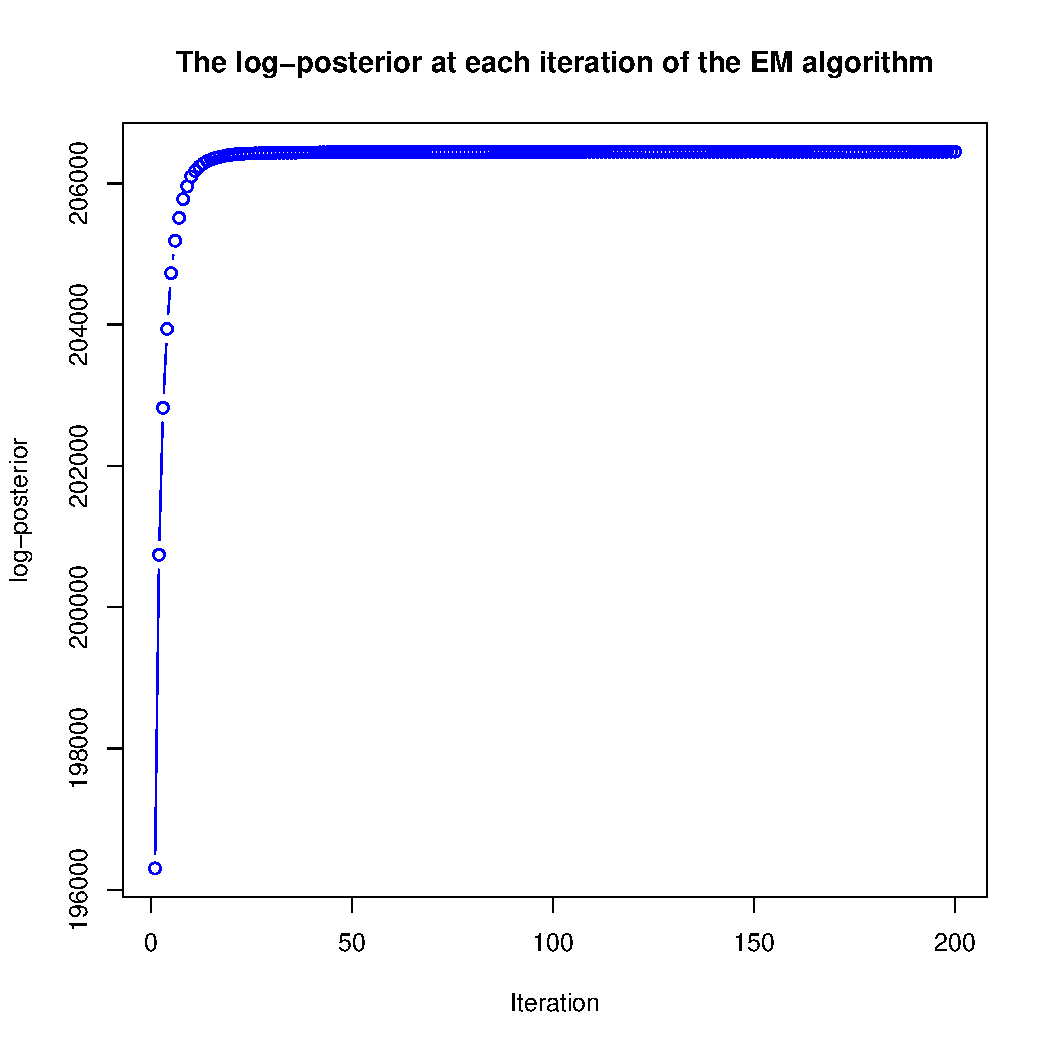
\includegraphics[width=0.6\textwidth]{figure/emconverge-1} 

\end{knitrout}

\caption{Plot of the log-posterior at each iteration of the EM
  algorithm to demonstrate monotonicity and convergence}
  \label{figure::emconvergence}
\end{figure}

\clearpage

\subsection{Appendix 4: Trace plots for assessing MCMC convergence}\label{app:mcmc}



\begin{figure}[ht]
  \centering
\begin{knitrout}
\definecolor{shadecolor}{rgb}{0.969, 0.969, 0.969}\color{fgcolor}
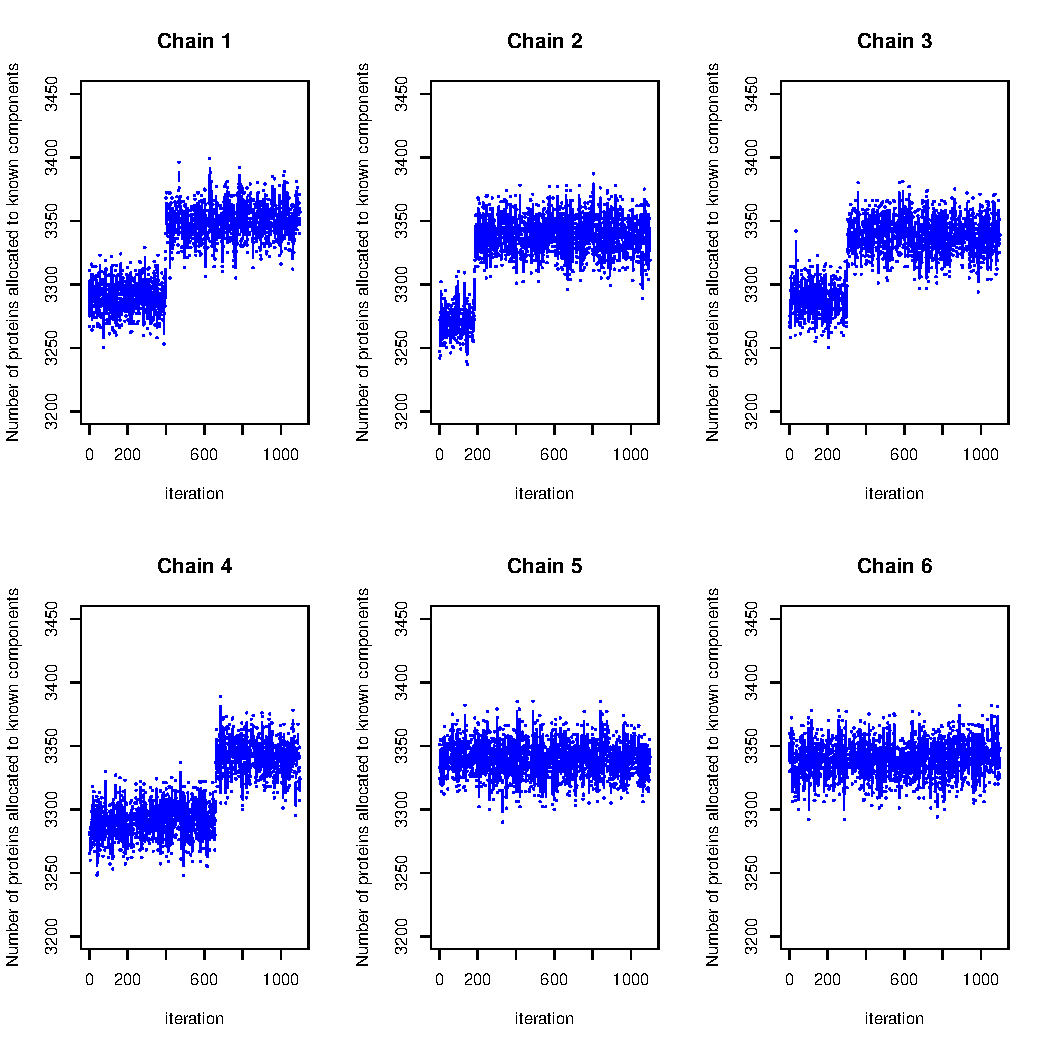
\includegraphics[width=0.75\textwidth]{figure/traceplots-1} 

\end{knitrout}
\caption{Trace plots of the number of proteins allocated to the known
  components in each of 6 parallel MCMC runs. Chain $4$ is discarded
  because of lack of convergence. $600$ samples are retained from
  remaining chains and pooled.}
  \label{figure::mcmcchains}
\end{figure}


\clearpage

\subsection{Appendix 5: F1 t-tests}\label{app::ttestf1}



% latex table generated in R 3.4.4 by xtable 1.8-2 package
% Fri May 18 18:37:29 2018
\begin{table}[ht]
\centering
\begin{tabular}{rrrr}
  \hline
 & SVM & KNN & MAP \\ 
  \hline
KNN & 2.7E-03 &  &  \\ 
  MAP & 3.3E-02 & 3.4E-01 &  \\ 
  MCMC & 3.4E-01 & 3.3E-02 & 2.3E-01 \\ 
   \hline
\end{tabular}
\caption{Adjusted P-values for pairwise T-tests for Macro F-1 score classifier evaluation on the Drosophila dataset} 
\end{table}
% latex table generated in R 3.4.4 by xtable 1.8-2 package
% Fri May 18 18:37:30 2018
\begin{table}[ht]
\centering
\begin{tabular}{rrrr}
  \hline
 & SVM & KNN & MAP \\ 
  \hline
KNN & 1.2E-02 &  &  \\ 
  MAP & 2.7E-01 & 1.5E-01 &  \\ 
  MCMC & 4.9E-01 & 1.9E-03 & 1.1E-01 \\ 
   \hline
\end{tabular}
\caption{Adjusted P-values for pairwise T-tests for Macro F-1 score classifier evaluation on the Chicken DT40 dataset} 
\end{table}
% latex table generated in R 3.4.4 by xtable 1.8-2 package
% Fri May 18 18:37:30 2018
\begin{table}[ht]
\centering
\begin{tabular}{rrrr}
  \hline
 & SVM & KNN & MAP \\ 
  \hline
KNN & 1.0E+00 &  &  \\ 
  MAP & 1.0E+00 & 1.0E+00 &  \\ 
  MCMC & 3.3E-01 & 6.0E-02 & 1.1E-05 \\ 
   \hline
\end{tabular}
\caption{Adjusted P-values for pairwise T-tests for Macro F-1 score classifier evaluation on the mouse dataset} 
\end{table}
% latex table generated in R 3.4.4 by xtable 1.8-2 package
% Fri May 18 18:37:30 2018
\begin{table}[ht]
\centering
\begin{tabular}{rrrr}
  \hline
 & SVM & KNN & MAP \\ 
  \hline
KNN & 1.4E-35 &  &  \\ 
  MAP & 3.3E-06 & 6.7E-21 &  \\ 
  MCMC & 8.0E-59 & 3.2E-91 & 2.4E-70 \\ 
   \hline
\end{tabular}
\caption{Adjusted P-values for pairwise T-tests for Macro F-1 score classifier evaluation on the HeLa dataset} 
\end{table}
% latex table generated in R 3.4.4 by xtable 1.8-2 package
% Fri May 18 18:37:30 2018
\begin{table}[ht]
\centering
\begin{tabular}{rrrr}
  \hline
 & SVM & KNN & MAP \\ 
  \hline
KNN & 1.3E-02 &  &  \\ 
  MAP & 4.3E-04 & 3.3E-09 &  \\ 
  MCMC & 5.8E-01 & 3.5E-03 & 3.1E-03 \\ 
   \hline
\end{tabular}
\caption{Adjusted P-values for pairwise T-tests for Macro F-1 score classifier evaluation on the U2-OS dataset} 
\end{table}
% latex table generated in R 3.4.4 by xtable 1.8-2 package
% Fri May 18 18:37:30 2018
\begin{table}[ht]
\centering
\begin{tabular}{rrrr}
  \hline
 & SVM & KNN & MAP \\ 
  \hline
KNN & 2.2E-08 &  &  \\ 
  MAP & 1.0E-34 & 6.8E-14 &  \\ 
  MCMC & 7.4E-05 & 5.3E-02 & 1.0E-20 \\ 
   \hline
\end{tabular}
\caption{Adjusted P-values for pairwise T-tests for Macro F-1 score classifier evaluation on the HeLa wild (Hirst et al.) dataset} 
\end{table}
% latex table generated in R 3.4.4 by xtable 1.8-2 package
% Fri May 18 18:37:30 2018
\begin{table}[ht]
\centering
\begin{tabular}{rrrr}
  \hline
 & SVM & KNN & MAP \\ 
  \hline
KNN & 5.3E-02 &  &  \\ 
  MAP & 1.7E-23 & 7.9E-27 &  \\ 
  MCMC & 9.1E-02 & 5.8E-04 & 1.8E-19 \\ 
   \hline
\end{tabular}
\caption{Adjusted P-values for pairwise T-tests for Macro F-1 score classifier evaluation on the HeLa KO1 (Hirst et al.) dataset} 
\end{table}
% latex table generated in R 3.4.4 by xtable 1.8-2 package
% Fri May 18 18:37:30 2018
\begin{table}[ht]
\centering
\begin{tabular}{rrrr}
  \hline
 & SVM & KNN & MAP \\ 
  \hline
KNN & 1.3E-01 &  &  \\ 
  MAP & 1.1E-55 & 1.1E-55 &  \\ 
  MCMC & 1.0E-18 & 6.3E-22 & 2.0E-26 \\ 
   \hline
\end{tabular}
\caption{Adjusted P-values for pairwise T-tests for Macro F-1 score classifier evaluation on the HeLa KO2 (Hirst et al.) dataset} 
\end{table}
% latex table generated in R 3.4.4 by xtable 1.8-2 package
% Fri May 18 18:37:30 2018
\begin{table}[ht]
\centering
\begin{tabular}{rrrr}
  \hline
 & SVM & KNN & MAP \\ 
  \hline
KNN & 9.6E-02 &  &  \\ 
  MAP & 4.1E-07 & 1.1E-09 &  \\ 
  MCMC & 2.8E-27 & 1.0E-28 & 6.3E-10 \\ 
   \hline
\end{tabular}
\caption{Adjusted P-values for pairwise T-tests for Macro F-1 score classifier evaluation on the Primary Fibroblasts Mock 24hpi dataset} 
\end{table}
% latex table generated in R 3.4.4 by xtable 1.8-2 package
% Fri May 18 18:37:30 2018
\begin{table}[ht]
\centering
\begin{tabular}{rrrr}
  \hline
 & SVM & KNN & MAP \\ 
  \hline
KNN & 6.6E-07 &  &  \\ 
  MAP & 1.3E-10 & 2.0E-01 &  \\ 
  MCMC & 1.6E-05 & 2.0E-01 & 6.2E-03 \\ 
   \hline
\end{tabular}
\caption{Adjusted P-values for pairwise T-tests for Macro F-1 score classifier evaluation on the Primary Fibroblasts Mock 48hpi dataset} 
\end{table}
% latex table generated in R 3.4.4 by xtable 1.8-2 package
% Fri May 18 18:37:30 2018
\begin{table}[ht]
\centering
\begin{tabular}{rrrr}
  \hline
 & SVM & KNN & MAP \\ 
  \hline
KNN & 3.9E-03 &  &  \\ 
  MAP & 9.5E-01 & 8.6E-03 &  \\ 
  MCMC & 6.4E-02 & 3.0E-01 & 8.6E-02 \\ 
   \hline
\end{tabular}
\caption{Adjusted P-values for pairwise T-tests for Macro F-1 score classifier evaluation on the Primary Fibroblasts Mock 72hpi dataset} 
\end{table}
% latex table generated in R 3.4.4 by xtable 1.8-2 package
% Fri May 18 18:37:30 2018
\begin{table}[ht]
\centering
\begin{tabular}{rrrr}
  \hline
 & SVM & KNN & MAP \\ 
  \hline
KNN & 8.6E-03 &  &  \\ 
  MAP & 1.1E-02 & 8.6E-01 &  \\ 
  MCMC & 3.7E-06 & 1.6E-02 & 3.3E-02 \\ 
   \hline
\end{tabular}
\caption{Adjusted P-values for pairwise T-tests for Macro F-1 score classifier evaluation on the Primary Fibroblasts Mock 96hpi dataset} 
\end{table}
% latex table generated in R 3.4.4 by xtable 1.8-2 package
% Fri May 18 18:37:30 2018
\begin{table}[ht]
\centering
\begin{tabular}{rrrr}
  \hline
 & SVM & KNN & MAP \\ 
  \hline
KNN & 1.9E-23 &  &  \\ 
  MAP & 1.4E-02 & 2.3E-34 &  \\ 
  MCMC & 3.8E-07 & 1.6E-81 & 2.0E-02 \\ 
   \hline
\end{tabular}
\caption{Adjusted P-values for pairwise T-tests for Macro F-1 score classifier evaluation on the Primary Fibroblasts Mock 120hpi dataset} 
\end{table}
% latex table generated in R 3.4.4 by xtable 1.8-2 package
% Fri May 18 18:37:30 2018
\begin{table}[ht]
\centering
\begin{tabular}{rrrr}
  \hline
 & SVM & KNN & MAP \\ 
  \hline
KNN & 4.6E-01 &  &  \\ 
  MAP & 2.6E-05 & 1.7E-04 &  \\ 
  MCMC & 1.7E-04 & 1.3E-03 & 5.5E-01 \\ 
   \hline
\end{tabular}
\caption{Adjusted P-values for pairwise T-tests for Macro F-1 score classifier evaluation on the Primary Fibroblasts HCMV 24hpi dataset} 
\end{table}
% latex table generated in R 3.4.4 by xtable 1.8-2 package
% Fri May 18 18:37:30 2018
\begin{table}[ht]
\centering
\begin{tabular}{rrrr}
  \hline
 & SVM & KNN & MAP \\ 
  \hline
KNN & 1.0E-02 &  &  \\ 
  MAP & 4.6E-01 & 1.5E-03 &  \\ 
  MCMC & 1.2E-02 & 7.3E-01 & 1.5E-03 \\ 
   \hline
\end{tabular}
\caption{Adjusted P-values for pairwise T-tests for Macro F-1 score classifier evaluation on the Primary Fibroblasts HCMV 48hpi dataset} 
\end{table}
% latex table generated in R 3.4.4 by xtable 1.8-2 package
% Fri May 18 18:37:30 2018
\begin{table}[ht]
\centering
\begin{tabular}{rrrr}
  \hline
 & SVM & KNN & MAP \\ 
  \hline
KNN & 5.5E-02 &  &  \\ 
  MAP & 9.5E-06 & 3.4E-02 &  \\ 
  MCMC & 1.1E-01 & 6.2E-01 & 6.4E-03 \\ 
   \hline
\end{tabular}
\caption{Adjusted P-values for pairwise T-tests for Macro F-1 score classifier evaluation on the Primary Fibroblasts HCMV 72hpi dataset} 
\end{table}
% latex table generated in R 3.4.4 by xtable 1.8-2 package
% Fri May 18 18:37:30 2018
\begin{table}[ht]
\centering
\begin{tabular}{rrrr}
  \hline
 & SVM & KNN & MAP \\ 
  \hline
KNN & 2.8E-01 &  &  \\ 
  MAP & 2.6E-09 & 7.2E-08 &  \\ 
  MCMC & 4.2E-10 & 5.6E-09 & 5.7E-01 \\ 
   \hline
\end{tabular}
\caption{Adjusted P-values for pairwise T-tests for Macro F-1 score classifier evaluation on the Primary Fibroblasts HCMV 96hpi dataset} 
\end{table}
% latex table generated in R 3.4.4 by xtable 1.8-2 package
% Fri May 18 18:37:30 2018
\begin{table}[ht]
\centering
\begin{tabular}{rrrr}
  \hline
 & SVM & KNN & MAP \\ 
  \hline
KNN & 2.3E-04 &  &  \\ 
  MAP & 7.1E-04 & 3.8E-10 &  \\ 
  MCMC & 1.4E-01 & 5.7E-02 & 6.0E-05 \\ 
   \hline
\end{tabular}
\caption{Adjusted P-values for pairwise T-tests for Macro F-1 score classifier evaluation on the Primary Fibroblasts HCMV 120hpi dataset} 
\end{table}
% latex table generated in R 3.4.4 by xtable 1.8-2 package
% Fri May 18 18:37:30 2018
\begin{table}[ht]
\centering
\begin{tabular}{rrrr}
  \hline
 & SVM & KNN & MAP \\ 
  \hline
KNN & 6.7E-06 &  &  \\ 
  MAP & 6.3E-05 & 4.4E-01 &  \\ 
  MCMC & 4.4E-01 & 6.7E-06 & 8.3E-05 \\ 
   \hline
\end{tabular}
\caption{Adjusted P-values for pairwise T-tests for Macro F-1 score classifier evaluation on the E14TG2a dataset} 
\end{table}


\clearpage
\subsection{Appendix 6: Quadratic loss t-tests}




% latex table generated in R 3.4.4 by xtable 1.8-2 package
% Fri May 18 18:37:30 2018
\begin{table}[ht]
\centering
\begin{tabular}{rrrr}
  \hline
 & SVM & KNN & MAP \\ 
  \hline
KNN & 5.9E-13 &  &  \\ 
  MAP & 1.1E-04 & 9.6E-124 &  \\ 
  MCMC & 2.2E-23 & 3.3E-58 & 5.9E-171 \\ 
   \hline
\end{tabular}
\caption{Adjusted P-values for pairwise T-tests for Quadratic Loss classifier evaluation on the Drosphila dataset} 
\end{table}
% latex table generated in R 3.4.4 by xtable 1.8-2 package
% Fri May 18 18:37:30 2018
\begin{table}[ht]
\centering
\begin{tabular}{rrrr}
  \hline
 & SVM & KNN & MAP \\ 
  \hline
KNN & 3.2E-08 &  &  \\ 
  MAP & 1.7E-26 & 1.3E-128 &  \\ 
  MCMC & 4.2E-13 & 8.8E-37 & 7.0E-135 \\ 
   \hline
\end{tabular}
\caption{Adjusted P-values for pairwise T-tests for Quadratic Loss classifier evaluation on the Chicken DT40 dataset} 
\end{table}
% latex table generated in R 3.4.4 by xtable 1.8-2 package
% Fri May 18 18:37:30 2018
\begin{table}[ht]
\centering
\begin{tabular}{rrrr}
  \hline
 & SVM & KNN & MAP \\ 
  \hline
KNN & 5.5E-14 &  &  \\ 
  MAP & 3.0E-25 & 6.3E-128 &  \\ 
  MCMC & 7.4E-26 & 1.7E-129 & 1.6E-14 \\ 
   \hline
\end{tabular}
\caption{Adjusted P-values for pairwise T-tests for Quadratic Loss classifier evaluation on the mouse dataset} 
\end{table}
% latex table generated in R 3.4.4 by xtable 1.8-2 package
% Fri May 18 18:37:30 2018
\begin{table}[ht]
\centering
\begin{tabular}{rrrr}
  \hline
 & SVM & KNN & MAP \\ 
  \hline
KNN & 1.2E-02 &  &  \\ 
  MAP & 9.4E-07 & 7.4E-86 &  \\ 
  MCMC & 5.5E-08 & 2.7E-89 & 2.4E-12 \\ 
   \hline
\end{tabular}
\caption{Adjusted P-values for pairwise T-tests for Quadratic Loss classifier evaluation on the HeLa dataset} 
\end{table}
% latex table generated in R 3.4.4 by xtable 1.8-2 package
% Fri May 18 18:37:30 2018
\begin{table}[ht]
\centering
\begin{tabular}{rrrr}
  \hline
 & SVM & KNN & MAP \\ 
  \hline
KNN & 6.8E-02 &  &  \\ 
  MAP & 7.4E-17 & 1.1E-73 &  \\ 
  MCMC & 1.4E-20 & 6.7E-81 & 8.3E-41 \\ 
   \hline
\end{tabular}
\caption{Adjusted P-values for pairwise T-tests for Quadratic Loss classifier evaluation on the U2-OS dataset} 
\end{table}
% latex table generated in R 3.4.4 by xtable 1.8-2 package
% Fri May 18 18:37:30 2018
\begin{table}[ht]
\centering
\begin{tabular}{rrrr}
  \hline
 & SVM & KNN & MAP \\ 
  \hline
KNN & 2.3E-92 &  &  \\ 
  MAP & 9.0E-13 & 2.4E-83 &  \\ 
  MCMC & 6.6E-19 & 3.0E-81 & 1.1E-01 \\ 
   \hline
\end{tabular}
\caption{Adjusted P-values for pairwise T-tests for Quadratic Loss classifier evaluation on the HeLa wild (Hirst et al.) dataset} 
\end{table}
% latex table generated in R 3.4.4 by xtable 1.8-2 package
% Fri May 18 18:37:30 2018
\begin{table}[ht]
\centering
\begin{tabular}{rrrr}
  \hline
 & SVM & KNN & MAP \\ 
  \hline
KNN & 5.2E-97 &  &  \\ 
  MAP & 1.4E-02 & 1.2E-90 &  \\ 
  MCMC & 2.3E-09 & 7.0E-95 & 2.2E-02 \\ 
   \hline
\end{tabular}
\caption{Adjusted P-values for pairwise T-tests for Quadratic Loss classifier evaluation on the HeLa KO1 (Hirst et al.) dataset} 
\end{table}
% latex table generated in R 3.4.4 by xtable 1.8-2 package
% Fri May 18 18:37:30 2018
\begin{table}[ht]
\centering
\begin{tabular}{rrrr}
  \hline
 & SVM & KNN & MAP \\ 
  \hline
KNN & 8.9E-93 &  &  \\ 
  MAP & 3.1E-01 & 8.1E-91 &  \\ 
  MCMC & 9.0E-06 & 1.5E-83 & 8.9E-05 \\ 
   \hline
\end{tabular}
\caption{Adjusted P-values for pairwise T-tests for Quadratic Loss classifier evaluation on the HeLa KO2 (Hirst et al.) dataset} 
\end{table}
% latex table generated in R 3.4.4 by xtable 1.8-2 package
% Fri May 18 18:37:31 2018
\begin{table}[ht]
\centering
\begin{tabular}{rrrr}
  \hline
 & SVM & KNN & MAP \\ 
  \hline
KNN & 6.1E-13 &  &  \\ 
  MAP & 1.4E-18 & 4.4E-81 &  \\ 
  MCMC & 3.2E-18 & 7.2E-77 & 5.9E-03 \\ 
   \hline
\end{tabular}
\caption{Adjusted P-values for pairwise T-tests for Quadratic Loss classifier evaluation on the Primary Fibroblasts Mock 24hpi dataset} 
\end{table}
% latex table generated in R 3.4.4 by xtable 1.8-2 package
% Fri May 18 18:37:31 2018
\begin{table}[ht]
\centering
\begin{tabular}{rrrr}
  \hline
 & SVM & KNN & MAP \\ 
  \hline
KNN & 6.1E-18 &  &  \\ 
  MAP & 3.6E-24 & 2.2E-57 &  \\ 
  MCMC & 1.4E-24 & 3.6E-61 & 3.6E-04 \\ 
   \hline
\end{tabular}
\caption{Adjusted P-values for pairwise T-tests for Quadratic Loss classifier evaluation on the Primary Fibroblasts Mock 48hpi dataset} 
\end{table}
% latex table generated in R 3.4.4 by xtable 1.8-2 package
% Fri May 18 18:37:31 2018
\begin{table}[ht]
\centering
\begin{tabular}{rrrr}
  \hline
 & SVM & KNN & MAP \\ 
  \hline
KNN & 1.2E-15 &  &  \\ 
  MAP & 4.5E-23 & 2.5E-89 &  \\ 
  MCMC & 4.2E-23 & 5.1E-91 & 4.4E-01 \\ 
   \hline
\end{tabular}
\caption{Adjusted P-values for pairwise T-tests for Quadratic Loss classifier evaluation on the Primary Fibroblasts Mock 72hpi dataset} 
\end{table}
% latex table generated in R 3.4.4 by xtable 1.8-2 package
% Fri May 18 18:37:31 2018
\begin{table}[ht]
\centering
\begin{tabular}{rrrr}
  \hline
 & SVM & KNN & MAP \\ 
  \hline
KNN & 1.8E-13 &  &  \\ 
  MAP & 1.4E-20 & 3.6E-126 &  \\ 
  MCMC & 5.0E-20 & 1.5E-109 & 5.3E-07 \\ 
   \hline
\end{tabular}
\caption{Adjusted P-values for pairwise T-tests for Quadratic Loss classifier evaluation on the Primary Fibroblasts Mock 96hpi dataset} 
\end{table}
% latex table generated in R 3.4.4 by xtable 1.8-2 package
% Fri May 18 18:37:31 2018
\begin{table}[ht]
\centering
\begin{tabular}{rrrr}
  \hline
 & SVM & KNN & MAP \\ 
  \hline
KNN & 6.7E-14 &  &  \\ 
  MAP & 1.0E-19 & 2.6E-45 &  \\ 
  MCMC & 8.0E-20 & 2.4E-45 & 2.5E-02 \\ 
   \hline
\end{tabular}
\caption{Adjusted P-values for pairwise T-tests for Quadratic Loss classifier evaluation on the Primary Fibroblasts Mock 120hpi dataset} 
\end{table}
% latex table generated in R 3.4.4 by xtable 1.8-2 package
% Fri May 18 18:37:31 2018
\begin{table}[ht]
\centering
\begin{tabular}{rrrr}
  \hline
 & SVM & KNN & MAP \\ 
  \hline
KNN & 6.0E-22 &  &  \\ 
  MAP & 2.8E-27 & 6.4E-53 &  \\ 
  MCMC & 1.4E-27 & 1.5E-56 & 3.0E-03 \\ 
   \hline
\end{tabular}
\caption{Adjusted P-values for pairwise T-tests for Quadratic Loss classifier evaluation on the Primary Fibroblasts HCMV 24hpi dataset} 
\end{table}
% latex table generated in R 3.4.4 by xtable 1.8-2 package
% Fri May 18 18:37:31 2018
\begin{table}[ht]
\centering
\begin{tabular}{rrrr}
  \hline
 & SVM & KNN & MAP \\ 
  \hline
KNN & 1.9E-26 &  &  \\ 
  MAP & 1.3E-33 & 2.7E-84 &  \\ 
  MCMC & 1.3E-33 & 2.7E-84 & 6.0E-01 \\ 
   \hline
\end{tabular}
\caption{Adjusted P-values for pairwise T-tests for Quadratic Loss classifier evaluation on the Primary Fibroblasts HCMV 48hpi dataset} 
\end{table}
% latex table generated in R 3.4.4 by xtable 1.8-2 package
% Fri May 18 18:37:31 2018
\begin{table}[ht]
\centering
\begin{tabular}{rrrr}
  \hline
 & SVM & KNN & MAP \\ 
  \hline
KNN & 6.3E-20 &  &  \\ 
  MAP & 1.9E-25 & 2.7E-57 &  \\ 
  MCMC & 1.2E-25 & 3.4E-58 & 1.5E-02 \\ 
   \hline
\end{tabular}
\caption{Adjusted P-values for pairwise T-tests for Quadratic Loss classifier evaluation on the Primary Fibroblasts HCMV 72hpi dataset} 
\end{table}
% latex table generated in R 3.4.4 by xtable 1.8-2 package
% Fri May 18 18:37:31 2018
\begin{table}[ht]
\centering
\begin{tabular}{rrrr}
  \hline
 & SVM & KNN & MAP \\ 
  \hline
KNN & 1.7E-25 &  &  \\ 
  MAP & 9.3E-32 & 1.9E-56 &  \\ 
  MCMC & 9.3E-32 & 1.2E-54 & 7.1E-01 \\ 
   \hline
\end{tabular}
\caption{Adjusted P-values for pairwise T-tests for Quadratic Loss classifier evaluation on the Primary Fibroblasts HCMV 96hpi dataset} 
\end{table}
% latex table generated in R 3.4.4 by xtable 1.8-2 package
% Fri May 18 18:37:31 2018
\begin{table}[ht]
\centering
\begin{tabular}{rrrr}
  \hline
 & SVM & KNN & MAP \\ 
  \hline
KNN & 6.5E-25 &  &  \\ 
  MAP & 5.3E-32 & 1.1E-71 &  \\ 
  MCMC & 7.1E-32 & 8.4E-71 & 5.7E-02 \\ 
   \hline
\end{tabular}
\caption{Adjusted P-values for pairwise T-tests for Quadratic Loss classifier evaluation on the Primary Fibroblasts HCMV 120hpi dataset} 
\end{table}
% latex table generated in R 3.4.4 by xtable 1.8-2 package
% Fri May 18 18:37:31 2018
\begin{table}[ht]
\centering
\begin{tabular}{rrrr}
  \hline
 & SVM & KNN & MAP \\ 
  \hline
KNN & 4.7E-04 &  &  \\ 
  MAP & 4.7E-21 & 1.5E-103 &  \\ 
  MCMC & 3.3E-12 & 1.8E-57 & 1.3E-137 \\ 
   \hline
\end{tabular}
\caption{Adjusted P-values for pairwise T-tests for Quadratic Loss classifier evaluation on the E14TG2a dataset} 
\end{table}


\clearpage

\subsection{Appendix 7: GO enrichment analysis figures}



\begin{figure}[h]
  \begin{subfigure}[t]{0.5\textwidth}
        \centering
  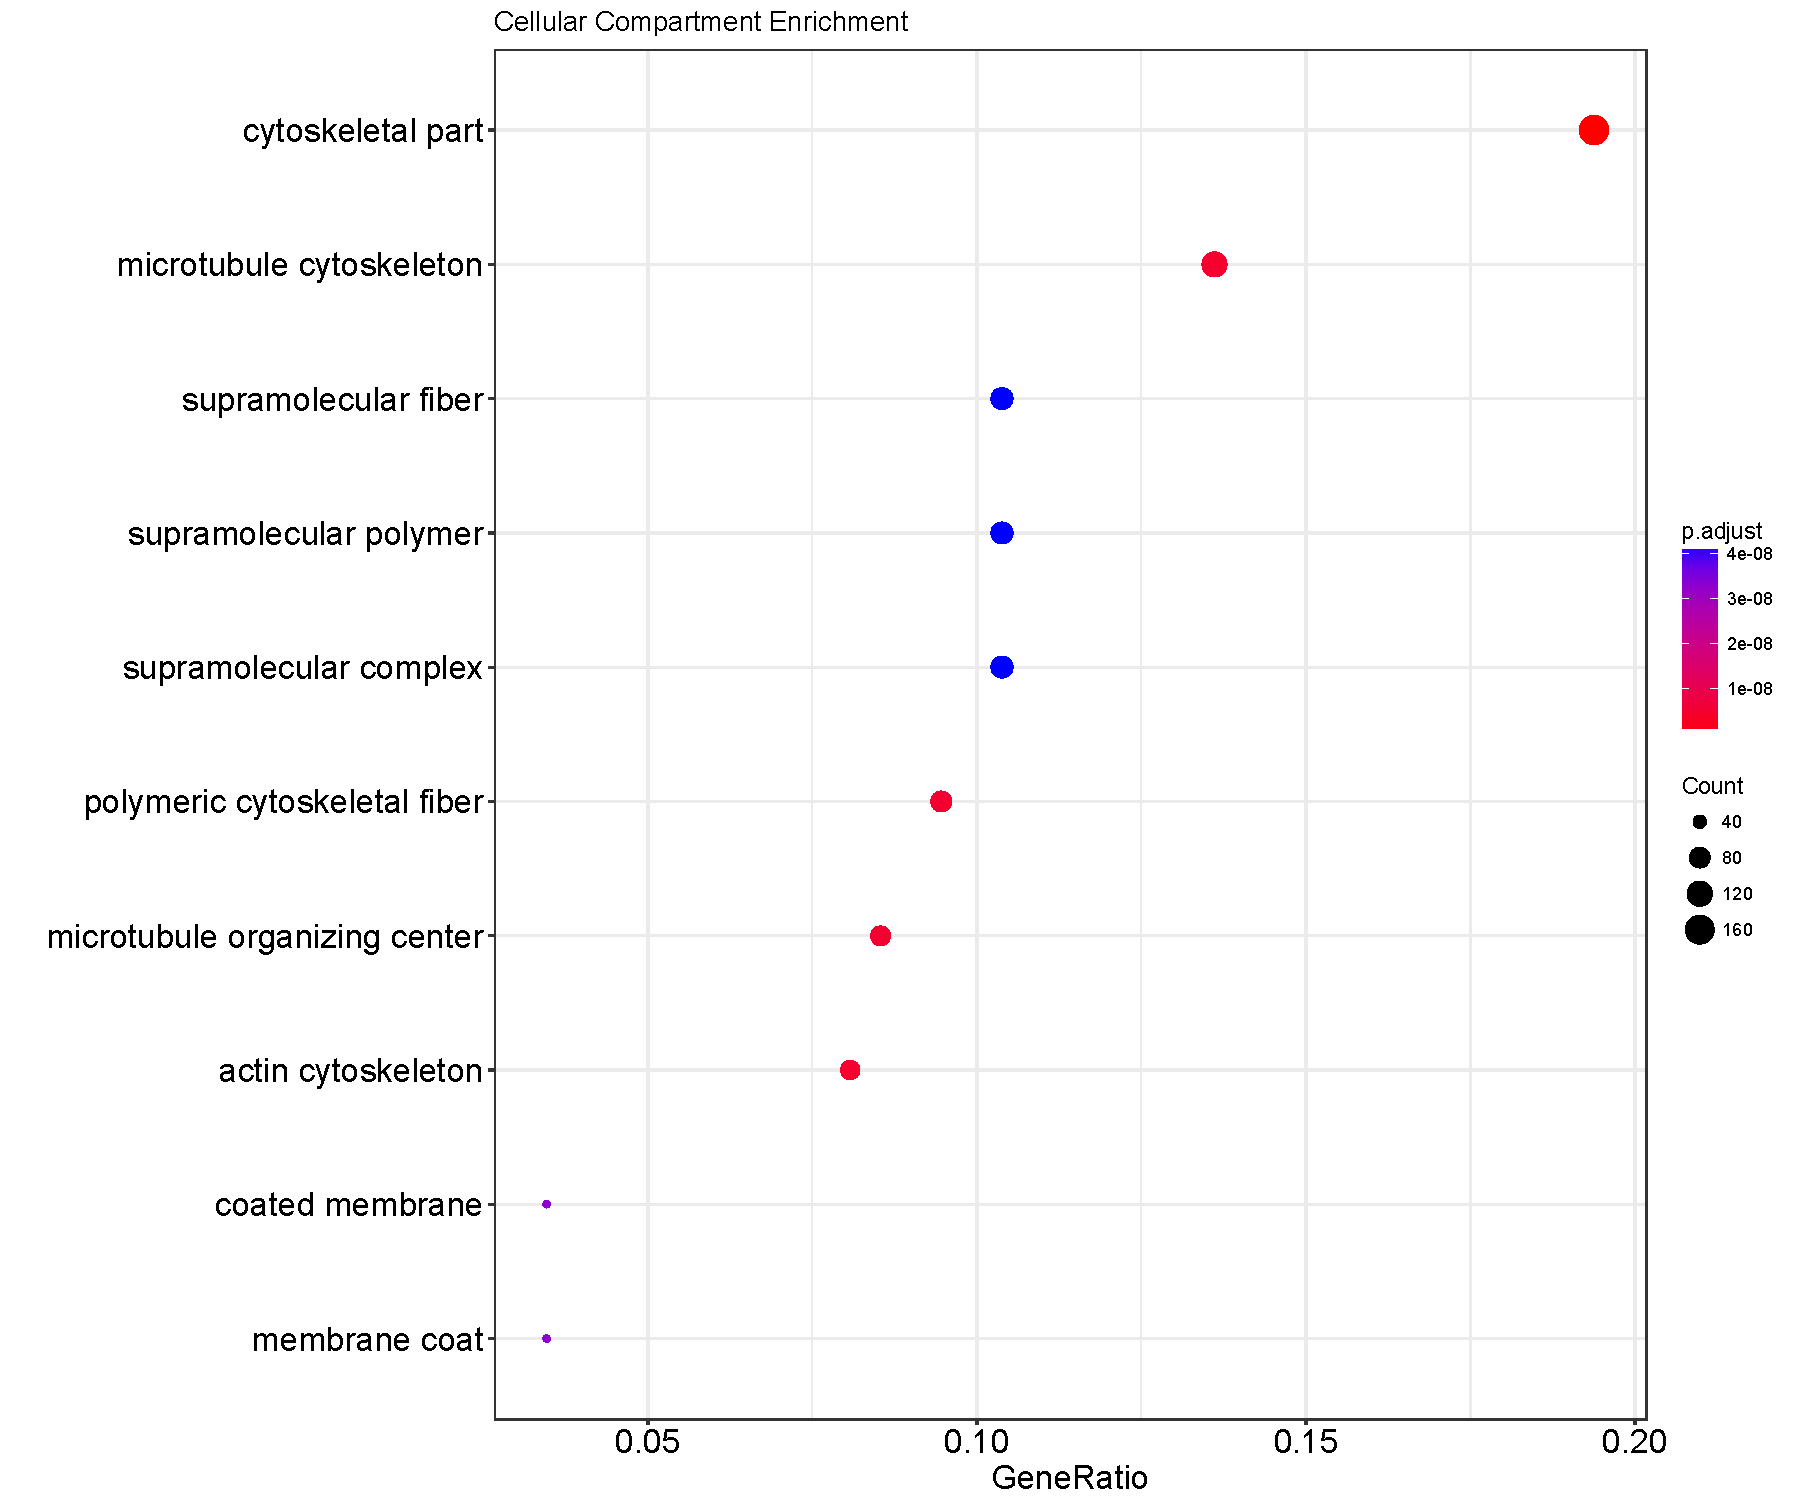
\includegraphics[width=\textwidth]{CCenrich.pdf}
        \caption{}
\end{subfigure}%
\begin{subfigure}[t]{0.5\textwidth}
\centering
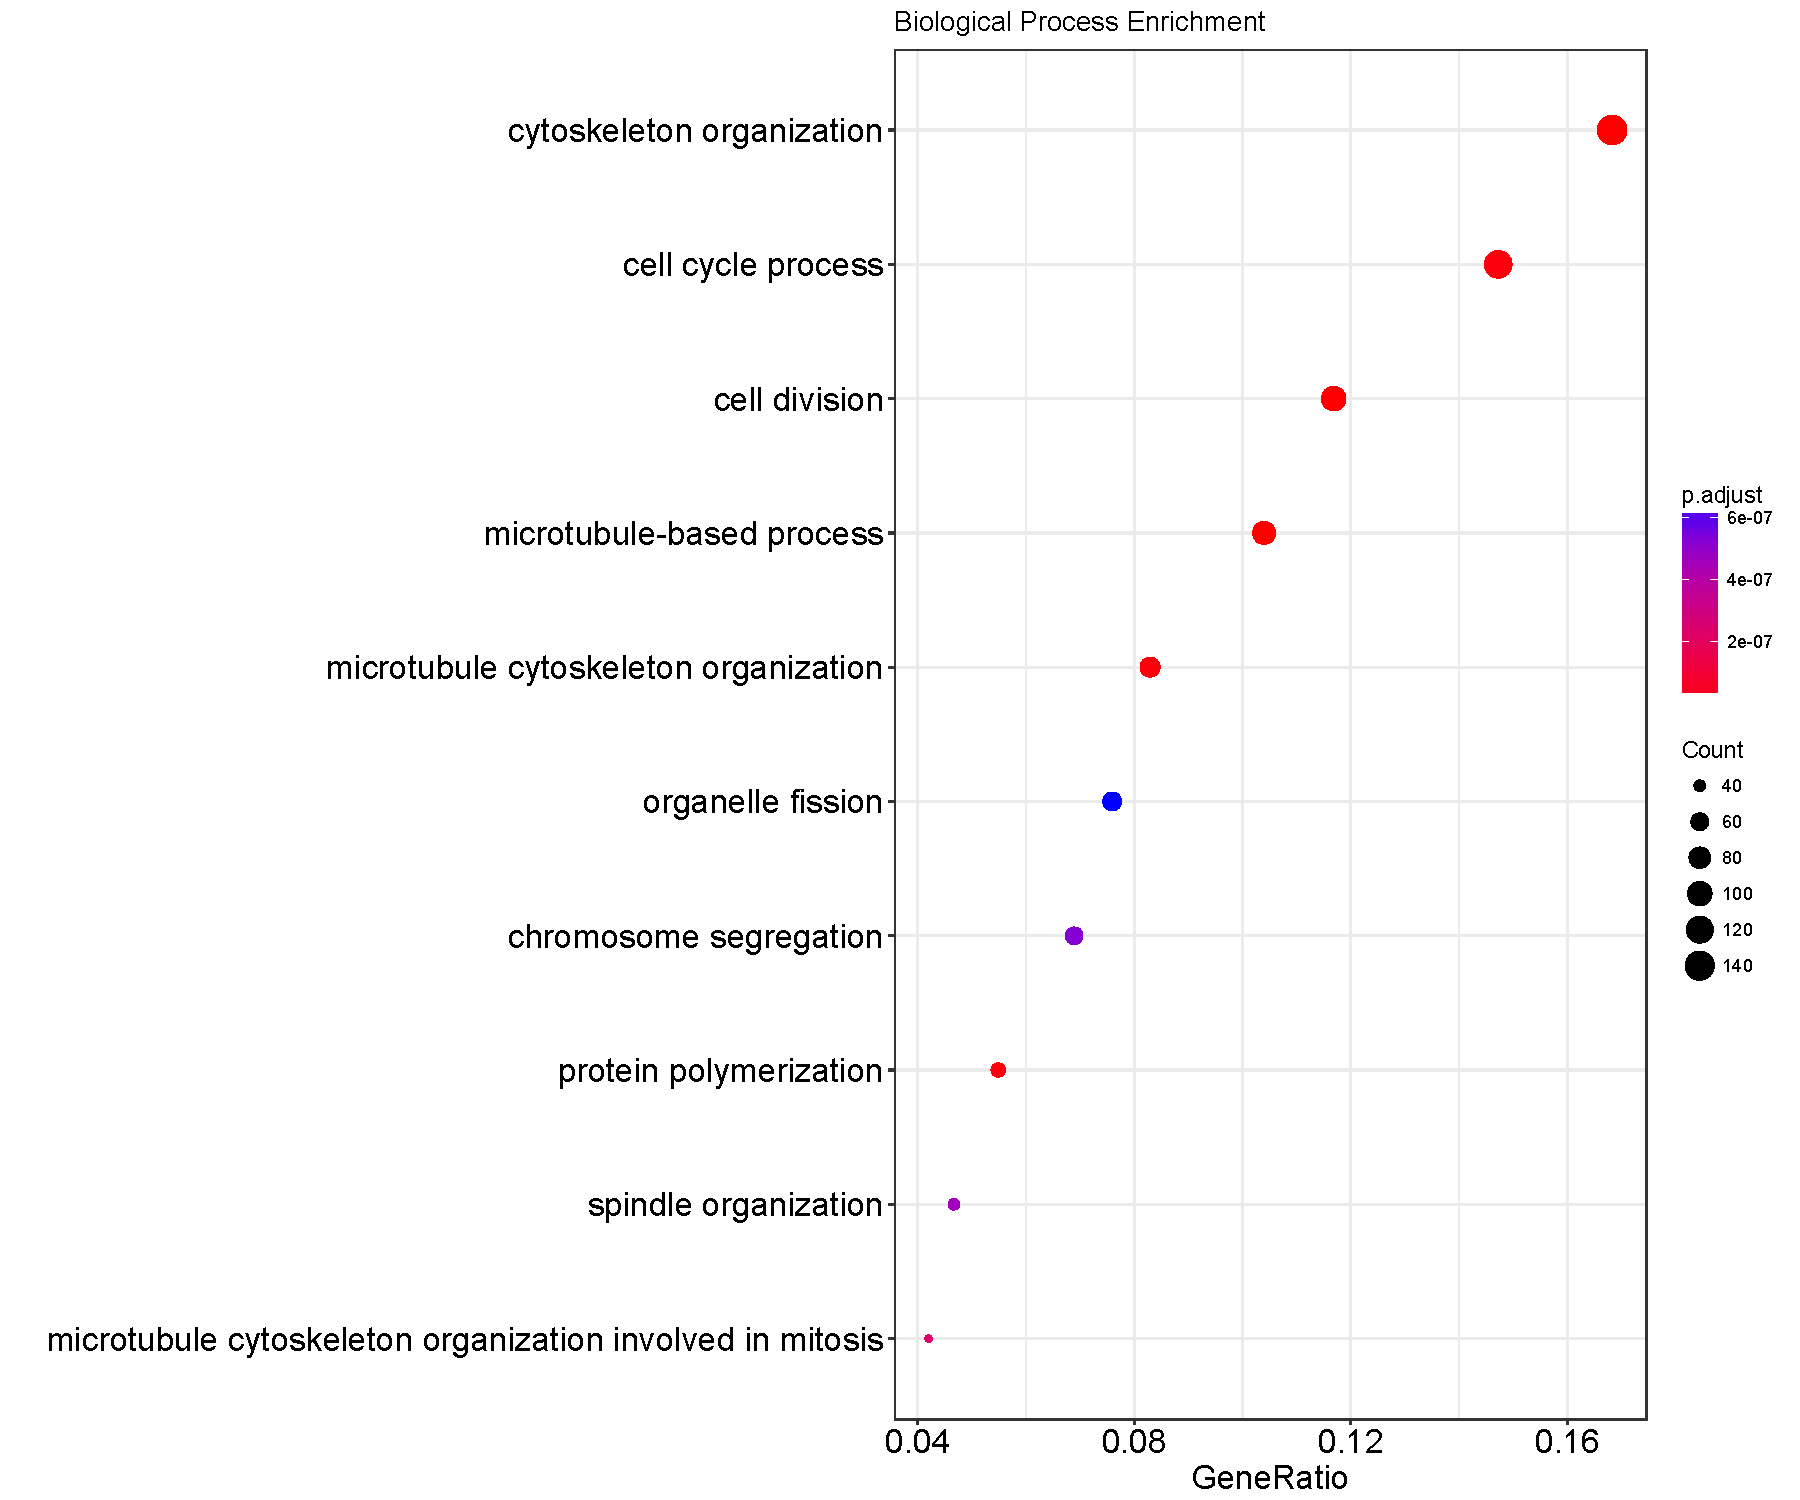
\includegraphics[width=\textwidth]{BPenrich.pdf}
        \caption{}
\end{subfigure}%
~

\begin{subfigure}[t]{0.5\textwidth}
\centering
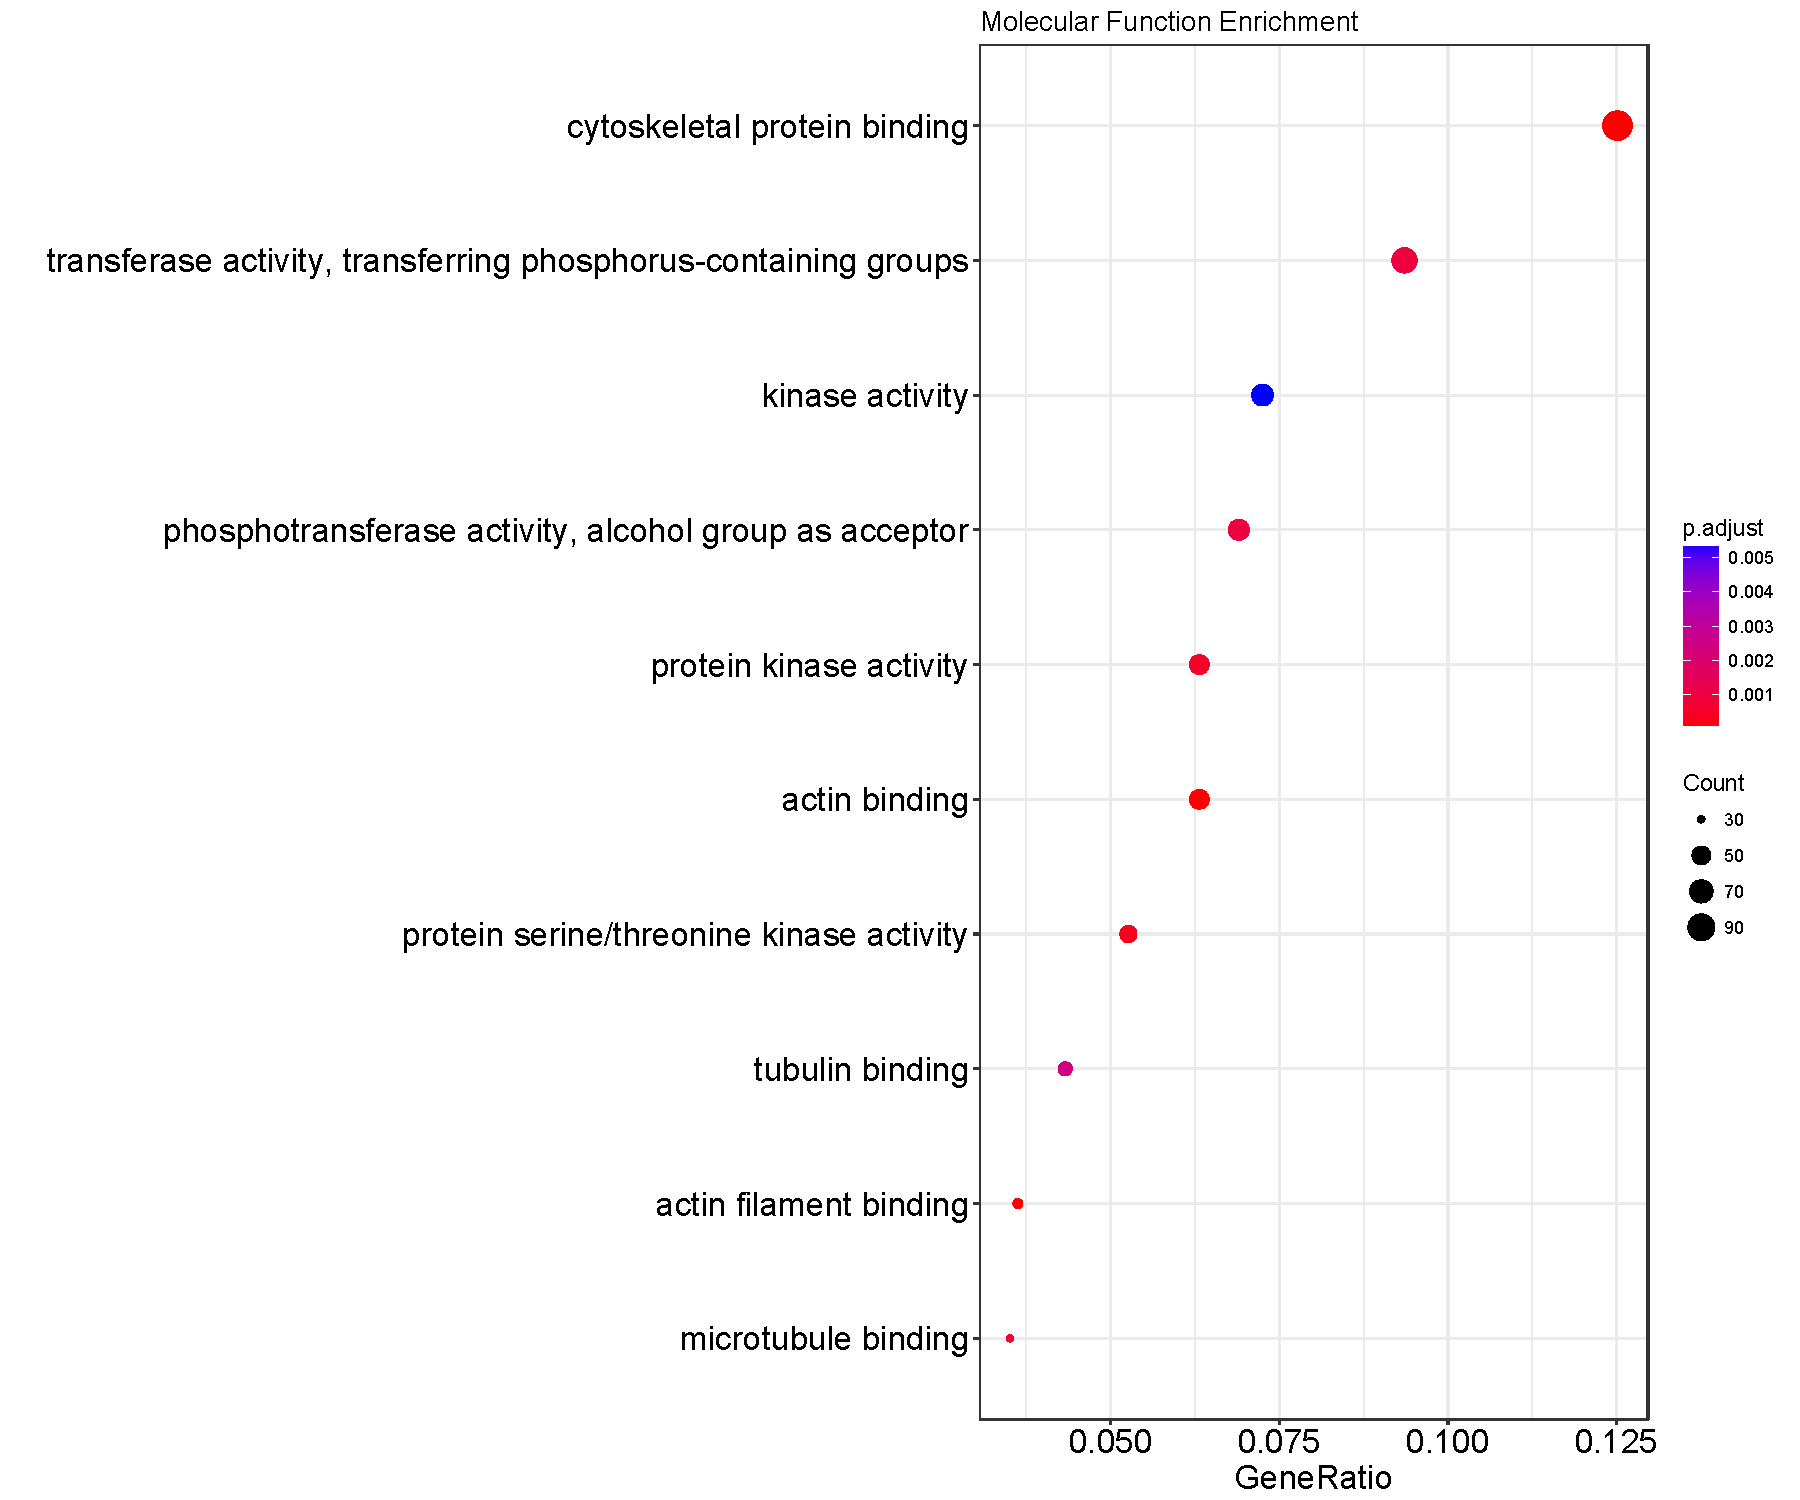
\includegraphics[width=\textwidth]{MFenrich.pdf}
        \caption{}
\end{subfigure}
\caption{Gene Ontology over representation analysis on outlier
  proteins - that is proteins allocated with less than probability
  $0.95$. We analyse the enrichment of terms in the cellular
  compartment, biological process, and molecular function
  ontologies. We display the top 10 significant results in the
  dotplots.}
\label{fig:GOenrich}
\end{figure}




\clearpage

\bibliographystyle{natbib}
\bibliography{BayesProt}


\end{document}
